%\documentclass[handout,ignorenonframetext,red]{beamer}
\documentclass[ignorenonframetext,red]{beamer}
%\documentclass[class=article, a4paper]{beamer}
%\documentclass[handout]{beamer} %pour sortie papier


\usepackage[french]{babel}
\usepackage{pgf,pgfarrows,pgfn odes,pgfautomata,pgfheaps,pgfs hade}
\usepackage{amsmath,amssymb}
\usepackage[utf8]{inputenc}
\usepackage{stmaryrd}
\usepackage{url}
\usepackage{wrapfig}
\usepackage{float}


%\documentclass[svgnames,ignorenonframetext]{beamer}
%\usepackage{times}
\usepackage{listings}
\usepackage{amsmath,multicol}
\usepackage{verbatim}
%\usepackage{beamerarticle}
\usepackage{longtable}
%\usepackage{ucs}
%\usepackage[utf8]{inputenc}
\usepackage{pdfpages}

\setcounter{tocdepth}{1}

\mode<presentation>
{
  \usetheme{Warsaw}
  \setbeamercovered{transparent}
  \AtBeginSection[]
  {
    \begin{frame}<beamer>
       \setcounter{tocdepth}{2}
       \tableofcontents[currentsection,currentsubsection,hideothersubsections]
    \end{frame}
  }

  \AtBeginSubsection[]
  {
    \begin{frame}<beamer>
    \frametitle{\thesection. \insertsectionhead}
       \tableofcontents[sectionstyle=hide/hide,subsectionstyle=show/shaded/hide ]
    \end{frame}
  }
  
  \addtobeamertemplate{footline}{\insertframenumber/\inserttotalframenumber}

}

%\mode<handout>{  \setbeamercolor{background canvas}{bg=black!5}} }


\logo{\vspace{-.10cm} \includegraphics[scale=0.1]{../illustration/logo_cnam.png}}
\date{\today}
\author{Rémi LEBLOND\\ \url{http://remileblond.fr}}
\institute{Conservatoire National des Arts et Métiers - Centre de Strasbourg}



\title{SMB137 - Quatrième partie}
\subtitle{Paradigmes de la concurrence}

\begin{document}
\frame[plain]{\titlepage}

\begin{frame}
 \frametitle{Plan}
 \tableofcontents
\end{frame}
 
\section{Coopération inter processus}
\subsection{Synchronisation de processus}

\begin{frame}
\frametitle{Synchronisation de processus}
\begin{itemize}
\item Problème :
\begin{itemize}
\item Un processus A, arrivé à un point X de son exécution, doit attendre qu'un processus B ait atteint ou dépassé un point Y de son exécution pour reprendre son travail
\end{itemize}
\item Solutions :
\begin{itemize}
\item Temporisation
\item Synchronisation
\end{itemize}
\end{itemize}
\begin{flushright}
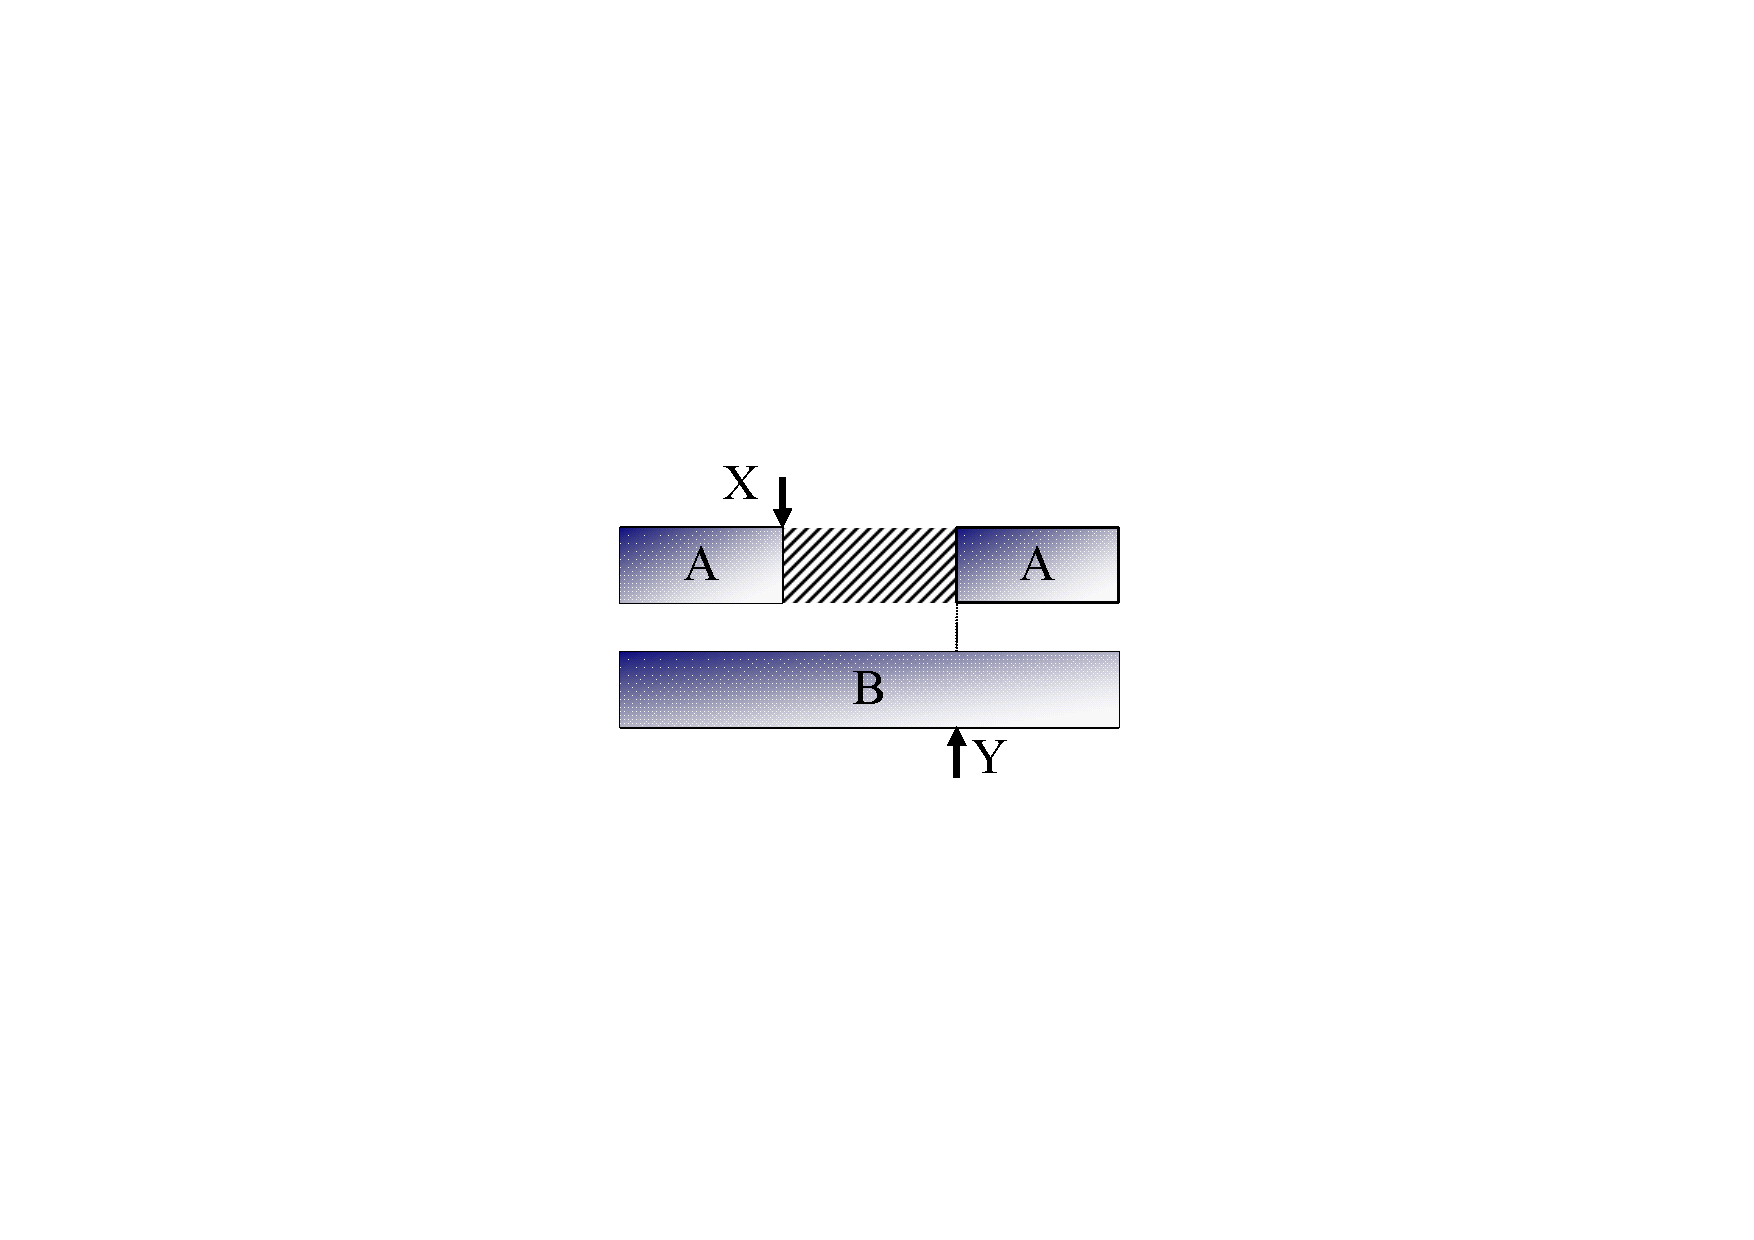
\includegraphics[width=.4\textwidth]{../illustration/temporisation.pdf}
\end{flushright}
\end{frame}

\begin{frame}
\frametitle{Approche par temporisation}
\framesubtitle{Solution risquée}
\begin{itemize}
\item Principe:
\begin{itemize}
\item Mesure le délai maximum D qu'il faut à B pour atteindre Y
\item Il suffit alors de commencer à exécuter A à partir de (début de B) + D
\end{itemize}
\item Problème:
\begin{itemize}
\item Solution difficile à ajuster et périlleuse
\item Mauvaise utilisation des ressources
\end{itemize}
\end{itemize}
\end{frame}

\begin{frame}
\frametitle{Approche par synchronisation}
\begin{itemize}
\item Utilisation de mécanismes de synchronisation :
\begin{itemize}
\item Par un processus pour signaler un événement aux autres processus
\end{itemize}
\item Doivent permettre
\begin{itemize}
\item l'auto-suspension d'un processus
\item l'activation d'un processus suspendu
\end{itemize}
\end{itemize}
\end{frame}

\begin{frame}
\frametitle{Synchronisation de processus}
\begin{itemize}
\item Processus coopérants
\item Partage de données
\begin{itemize}
\item Accès concurrents
\item Risque d’incohérence de données
\end{itemize}
\item Nécessité de synchronisation des processus concurrents
\end{itemize}
\end{frame}

\begin{frame}
\frametitle{Exemple : Producteur consommateur}
\begin{itemize}
\item Mémoire partagée
\item Tampon borné partagé
\begin{itemize}
\item Tableau circulaire avec deux pointeurs logiques :
\begin{itemize}
\item \texttt{in} : Pointe sur la position libre suivante du tampon
\item \texttt{out} : Pointe sur la première position pleine dans le tampon
\end{itemize}
\item Compteur :
\begin{itemize}
\item \texttt{count} : Nombre d’éléments contenus dans le tampon
\end{itemize}
\end{itemize}
\end{itemize}
\end{frame}

\begin{frame}
\frametitle{Producteur - consommateur : le tampon}
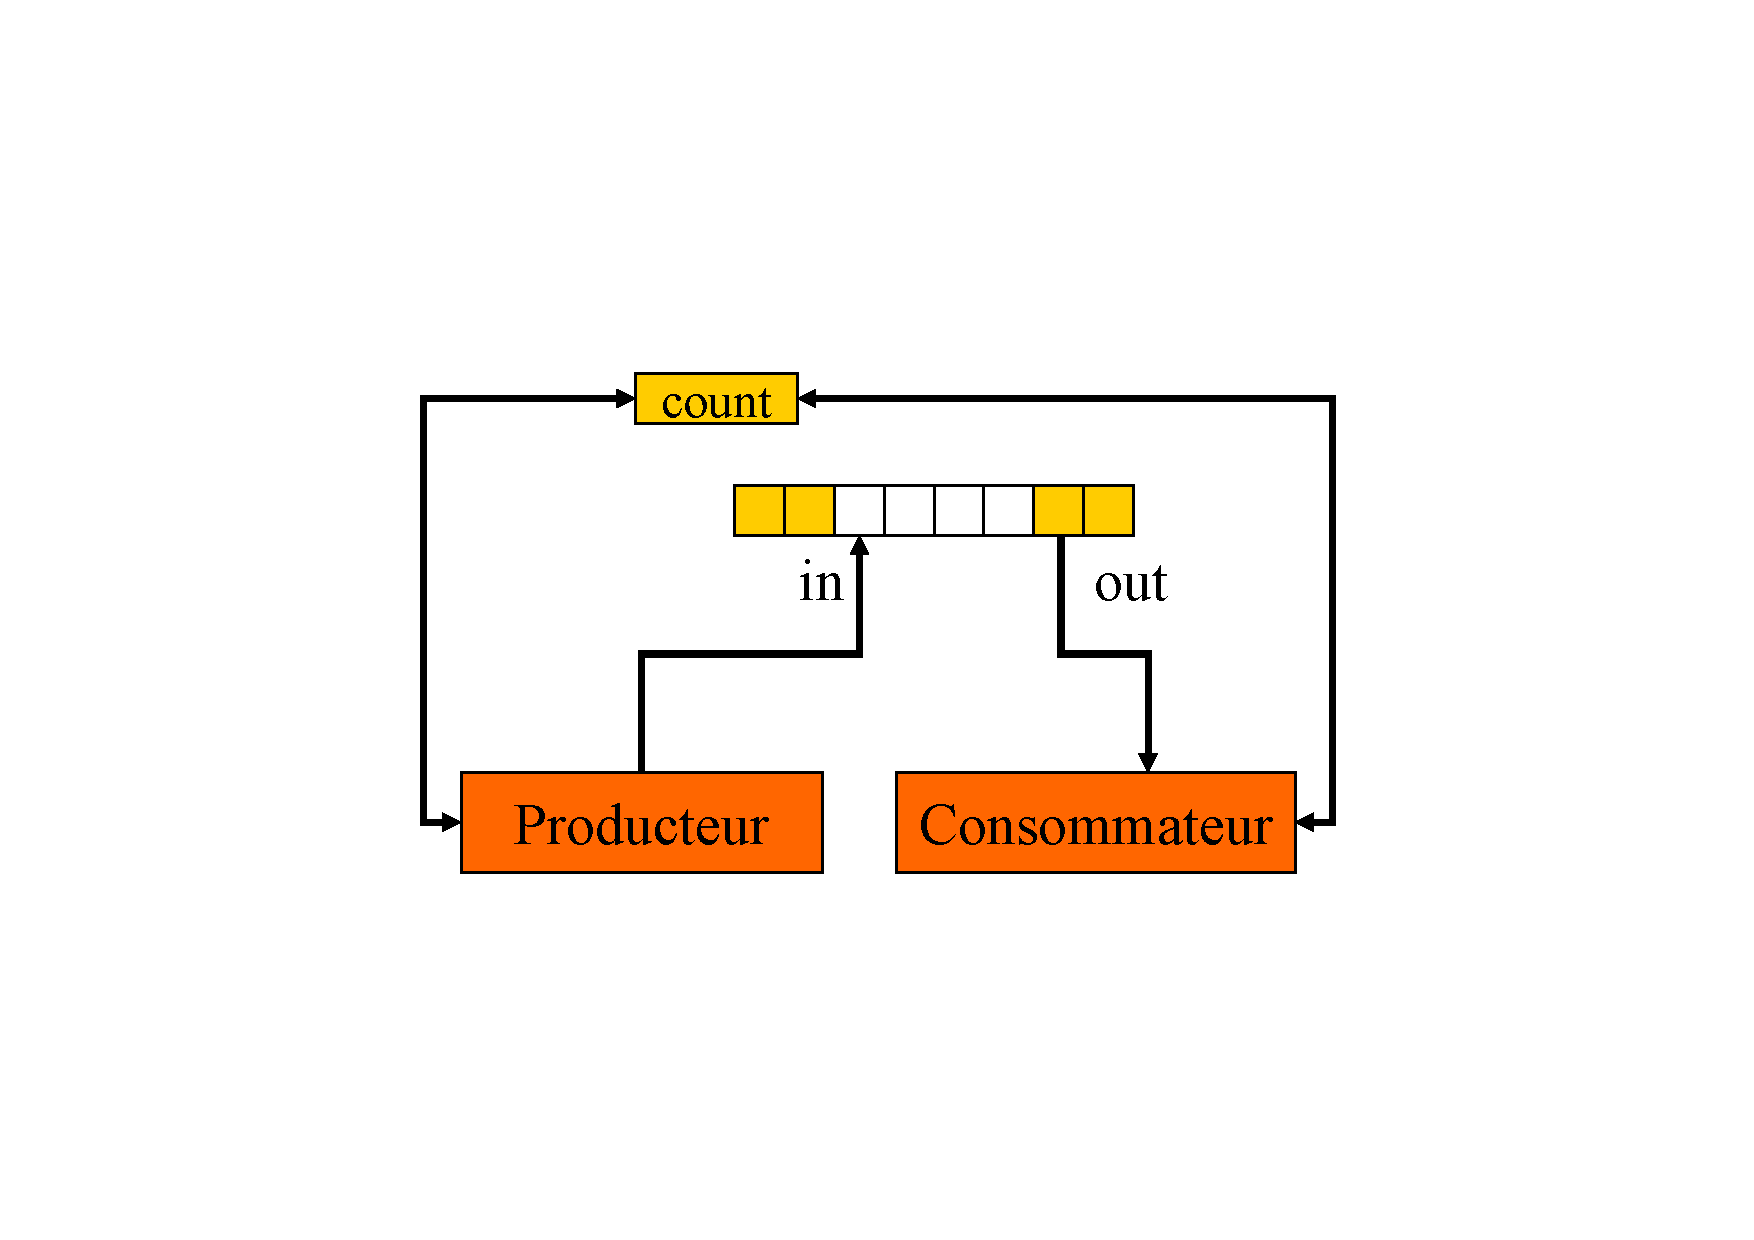
\includegraphics[width=.9\textwidth]{../illustration/prod_consom_tampon.pdf}
\end{frame}

\begin{frame}
\frametitle{Exemple : Producteur consommateur}
\begin{columns}
\column{0.45\textwidth}
\begin{block}{Producteur}
\begin{scriptsize}\verbatiminput{include/producteur.c}\end{scriptsize}
\end{block}
\column{0.45\textwidth}
\begin{block}{Consommateur}
\begin{scriptsize}
\verbatiminput{include/consommateur.c}
\end{scriptsize}
\end{block}
\end{columns}
\end{frame}

\subsection{Section critique}

\begin{frame}
\frametitle{Producteur consommateur }
\framesubtitle{Structure générale de l'implémentation logicielle}
\begin{scriptsize}\verbatiminput{include/sc_pc_archi.c}\end{scriptsize}
\end{frame}

\begin{frame}
\frametitle{Producteur - consommateur}
\framesubtitle{Méthode \texttt{ajouter()}}
\begin{scriptsize}\verbatiminput{include/sc_pc_ajouter.c}\end{scriptsize}
\end{frame}

\begin{frame}
\frametitle{Producteur - consommateur}
\framesubtitle{Méthode \texttt{retirer()}}
\begin{scriptsize}\verbatiminput{include/sc_pc_retirer.c}\end{scriptsize}
\end{frame}

\begin{frame}
\frametitle{Producteur - consommateur}
\framesubtitle{Implémentation du tampon}
\begin{scriptsize}\verbatiminput{include/sc_pc_tampon.c}\end{scriptsize}
\end{frame}

\begin{frame}
\frametitle{Exemple de processus concurrents}
\begin{itemize}
\item Algorithmes corrects pris individuellement
\item Partage de variables
\begin{itemize}
\item \texttt{count}
\item \texttt{tampon}
\item \texttt{in} et \texttt{out}
\end{itemize}
\item Risque d ’erreur lors de l’exécution simultanée
\begin{itemize}
\item Mise à jour des variables partagées
\end{itemize}
\end{itemize}
\end{frame}

\begin{frame}
\frametitle{Mise à jour des variables}

\begin{columns}
\column{0.45\textwidth}
\begin{block}{Producteur 1}
\begin{itemize}
\item $count++$
\item $tampon[in] = item$
\item $in = (in + 1) \% TAILLE\_TAMPON$
\end{itemize}
\end{block}

\column{0.45\textwidth}
\begin{block}{Producteur 2}
\begin{itemize}
\item $count++$
\item $tampon[in] = item$
\item $in = (in + 1) \% TAILLE\_TAMPON$
\end{itemize}
\end{block}
\end{columns}
\end{frame}

\begin{frame}
\frametitle{Problème de la section critique}
\begin{itemize}
\item Les données perdent leur cohérence si plusieurs producteurs et/ou consommateurs mettent à jour les variables \texttt{in}, \texttt{out}, \texttt{count} et le tableau \texttt{tampon} de manière concurrente
\item Besoin :
\begin{itemize}
\item Mettre en place des mécanismes permettant d’assurer qu’un seul processus à la fois ne peut manipuler ces variables
\item Mise à jour atomique de cet ensemble de données
\item Synchronisation des processus
\end{itemize}
\end{itemize}
\end{frame}

\begin{frame}
\frametitle{Problème de la section critique}
\begin{itemize}
\item La mise à jour des variables \texttt{in}, \texttt{out}, \texttt{count} et le tableau \texttt{tampon} doit se faire en \textbf{exclusion mutuelle}
\item Un seul thread à la fois modifie ces variables
\item L'autre doit attendre que le thread en cours ait fini
\end{itemize}
\begin{flushright}
\includegraphics[width=.5\textwidth]{../illustration/sc_maj_count.pdf}
\end{flushright}
\begin{itemize}
\item Il s’agit d’une \textbf{section critique}
\end{itemize}
\end{frame}

\begin{frame}
\frametitle{Qu'est-ce qu'une section critique ?}
\begin{block}{Définition d'une section critique}
Ensemble d'instructions pouvant produire des résultats imprévisibles lorsqu’il est exécuté simultanément par des processus/threads différents
\end{block}
\begin{itemize}
\item Partie délimitée du code
\item Relative à d'autres suites d'instructions sur les mêmes variables partagées (non dans l'absolu)
\end{itemize}
\end{frame}

\begin{frame}
\frametitle{Portée des sections critiques}
\begin{itemize}
\item L'exécution simultanée de deux sections critiques appartenant à des \textbf{ensembles différents} et ne partageant pas de variable ne pose pas de problème
\item Détermination des sections critiques :
\begin{itemize}
\item Liée à l’utilisation de variables partagées, mais l'inverse n'est pas systématiquement vrai
\item Doivent être détectées et protégées par les concepteurs des programmes
\end{itemize}
\end{itemize}
\end{frame}

\begin{frame}
\frametitle{Protection des sections critiques}
\framesubtitle{Protocoles d’entrée et de sortie}
\begin{block}{\textbf{Protocole d'entrée} en section critique}
Ensemble d'instructions qui permet cette vérification et la non-progression éventuelle
\end{block}
\begin{block}{\textbf{Protocole de sortie} de section critique}
Ensemble d'instructions qui permet à un processus ayant terminé sa section critique d'avertir d'autres processus en attente que la voie est libre
\end{block}
\end{frame}

\begin{frame}
\frametitle{Utilisation d’une section critique}
\begin{itemize}
\item \colorbox{green}{\textit{Section non critique}}
\item Protocole d'entrée en section critique
\item \colorbox{red}{\textit{Section critique}}
\item Protocole de sortie de section critique
\item \colorbox{green}{\textit{Section non critique}}
\end{itemize}
\end{frame}

\begin{frame}
\frametitle{Risques liés aux sections critiques}
\begin{columns}
\column{0.45\textwidth}
\textbf{Processus 1} :
\begin{itemize}
\item Entrée sect. critique 1
\item Entrée sect. critique 2

\centering{\texttt{Blocage}}

\item Sortie sect. critique 2
\item Sortie sect. critique 1
\end{itemize}
\column{0.45\textwidth}
\textbf{Processus 2} :
\begin{itemize}
\item Entrée sect. critique 2
\item Entrée sect. critique 1

\centering{\texttt{Blocage}}

\item Sortie sect. critique 1
\item Sortie sect. critique 2
\end{itemize}
\end{columns}
\begin{block}{}
\begin{center}
\textbf{Interblocage} des processus 1 et 2

\textbf{Étreinte fatale }(\textit{dead lock})
\end{center}
\end{block}
\end{frame}

\begin{frame}
\frametitle{Famine et équité}
\begin{itemize}
\item Risque de \textbf{famine} :
\begin{itemize}
\item Si un processus peut attendre indéfiniment pour entrer dans sa section critique alors que les autres exécutent normalement les leurs
\end{itemize}
\item Solution \textbf{équitable} si :
\begin{itemize}
\item Lorsqu'un processus A a demandé à entrer en section critique, il existe une borne supérieure au nombre de fois qu'un autre processus B peut entrer dans sa section critique avant que A n'entre dans la sienne
\end{itemize}
\end{itemize}
\end{frame}

\begin{frame}
\frametitle{Protection des sections critiques}
\begin{itemize}
\item Contraintes à satisfaire :
\begin{itemize}
\item Exclusion mutuelle
\item Déroulement
\item Attente bornée
\end{itemize}
\end{itemize}
\end{frame}

\begin{frame}
\frametitle{Contraintes à satisfaire :}
\begin{itemize}
\item \textbf{Exclusion mutuelle} :
\begin{itemize}
\item Une section critique ne peut être exécutée que si aucune autre section critique du même ensemble n'est en cours d'exécution
\item Dans le cas contraire, il devra attendre que l'autre processus termine sa section critique
\end{itemize}
\end{itemize}
\end{frame}

\begin{frame}
\frametitle{Contraintes à satisfaire :}
\begin{itemize}
\item \textbf{Déroulement} :
\begin{itemize}
\item Le choix du prochain processus pouvant entrer dans sa section critique ne peut se faire que parmi les processus qui n’exécutent pas déjà leur section critique.
\item Ce choix ne peut pas être repoussé indéfiniment
\end{itemize}
\end{itemize}
\end{frame}

\begin{frame}
\frametitle{Contraintes à satisfaire :}
\begin{itemize}
\item \textbf{Attente bornée} :
\begin{itemize}
\item Il existe une borne au nombre de thread pouvant entrer successivement en section critique après qu’un thread ait demandé l’accès à la section critique.
\item Cette borne empêche la \textbf{famine}.
\end{itemize}
\end{itemize}
\end{frame}


\begin{frame}
\frametitle{Exemple avec Java}
\framesubtitle{Protection des sections critiques}
\begin{itemize}
\item 4 classes :
\begin{itemize}
\item [exclusionMutuelle] Classe abstraite de mécanisme de protection de section critique
\item [travailleur] Thread comportant une section critique
\item [algo] Hérite de exclusionMutuelle, implémentation d ’un mécanisme de protection de section critique
\item [test] Lancement des travailleurs
\end{itemize}
\end{itemize}
\end{frame}

\begin{frame}
\frametitle{Classe « exclusionMutuelle »}
\begin{scriptsize}\verbatiminput{include/exclusionMutuelle.java}\end{scriptsize}
\end{frame}

\begin{frame}
\frametitle{Classe « travailleur »}
\begin{scriptsize}\verbatiminput{include/travailleur.java}\end{scriptsize}
\end{frame}

\begin{frame}
\frametitle{1$^{ere}$ solution logicielle}
\begin{itemize}
\item Variable commune signalant l’occupation de la section critique (verrou)
\item Entrée dans la section critique si le verrou n’est pas posé
\item Positionnement du verrou lors de l’entrée en section critique
\item Libération du verrou lors de la sortie de la section critique
\end{itemize}
\end{frame}

\begin{frame}
\frametitle{1$^{ere}$ solution logicielle}
\begin{scriptsize}\verbatiminput{include/algo1.java}\end{scriptsize}
\end{frame}

\begin{frame}
\frametitle{1$^{ere}$ solution logicielle}
\begin{columns}
\column{0.8\textwidth}
\begin{scriptsize}\verbatiminput{include/test1.java}\end{scriptsize}
\column{0.2\textwidth}
\begin{itemize}
\begin{scriptsize}
\item 0 ? SC
\item 0 $\rightarrow$ SC
\item 1 ? SC
\item 0 $\leftarrow$ SC
\item 0 ? SC
\item 0 $\rightarrow$ SC
\item 0 $\leftarrow$ SC
\item 1 $\rightarrow$ SC
\item 0 ? SC
\item \textit{Fin de 0}
\item 1 $\leftarrow$ SC
\item 1 ? SC
\item 1 $\rightarrow$ SC
\item 1 $\leftarrow$ SC
\item ...
\end{scriptsize}
\end{itemize}
\end{columns}
\end{frame}

\begin{frame}
\frametitle{1$^{ere}$ solution logicielle}
\framesubtitle{Avantages / inconvénients}
\begin{columns}
\column{0.45\textwidth}
\begin{block}{Avantages}
\begin{itemize}
\item Satisfait la condition d’exclusion mutuelle
\begin{itemize}
\item Attention de ne pas créer une section critique sur le test / set du verrou
\end{itemize}

\end{itemize}
\end{block}
\column{0.45\textwidth}
\begin{block}{Inconvénients}
\begin{itemize}
\item Ne satisfait pas la condition de déroulement
\item Ne satisfait pas la condition d’attente bornée
\item La consultation et la modification de la variable commune occupé constituent elles-mêmes de nouvelles sections critiques
\end{itemize}
\end{block}
\end{columns}
\end{frame}

\begin{frame}
\frametitle{1$^{ere}$ solution logicielle}
\begin{itemize}
\item Dans les anciennes versions d’Unix
\begin{itemize}
\item Variable de verrouillage :
\begin{itemize}
\item Fichier sans droit créé dans le protocole d’accès
\item Supprimé dans le protocole de sortie
\end{itemize}
\end{itemize}
\item Maintenant :
\begin{itemize}
\item Verrouillage d’un fichier
\begin{itemize}
\item Fonction \texttt{flock(descripteur, mode)}
\item \textit{où mode = \texttt{LOCK\_EX} ou \texttt{LOCK\_UN}}
\end{itemize}
\end{itemize}
\end{itemize}
\end{frame}

\begin{frame}
\frametitle{1$^{ere}$ solution logicielle}
\framesubtitle{Application avec Unix - utilisation d'un fichier en tant que verrou}
\begin{scriptsize}\verbatiminput{include/1sol_logiciel_unix.c}\end{scriptsize}
\end{frame}

\begin{frame}
\frametitle{2$^{eme}$ solution logicielle}
\begin{itemize}
\item Utilisation d’une variable donnant le nom du prochain Thread pouvant entrer en section critique (0 ou 1)
\item \textbf{Alternance} entre les Threads en concurrence
\end{itemize}
\end{frame}

\begin{frame}
\frametitle{2$^{eme}$ solution logicielle}
\begin{scriptsize}\verbatiminput{include/algo2.java}\end{scriptsize}
\end{frame}

\begin{frame}
\frametitle{2$^{eme}$ solution logicielle}
\begin{columns}
\column{0.8\textwidth}
\begin{scriptsize}\verbatiminput{include/test2.java}\end{scriptsize}
\column{0.2\textwidth}
\begin{itemize}
\begin{scriptsize}
\item 0 ? SC
\item 0 $\rightarrow$ SC
\item 1 ? SC
\item 0 $\leftarrow$ SC
\item 1 $\rightarrow$ SC
\item 0 ? SC
\item \textit{Fin de 0}
\item 1 $\leftarrow$ SC
\item 1 ? SC
\item \textbf{Blocage}
\end{scriptsize}
\end{itemize}
\end{columns}
\end{frame}

\begin{frame}
\frametitle{2$^{eme}$ solution logicielle}
\framesubtitle{Avantages / inconvénients}
\begin{columns}
\column{0.45\textwidth}
\begin{block}{Avantages}
\begin{itemize}
\item Exclusion mutuelle
\item Déroulement
\end{itemize}
\end{block}
\column{0.45\textwidth}
\begin{block}{Inconvénients}
\begin{itemize}
\item Attente non bornée
\item Impose une stricte alternance entre les deux Threads
\end{itemize}
\end{block}
\end{columns}
\end{frame}

\begin{frame}
\frametitle{3$^{eme}$ solution logicielle}
\begin{itemize}
\item Tableau de l’état des demandes d’entrée en section critique
\item Une entrée par Thread concurrent
\item Positionné, pour chaque Thread :
\begin{itemize}
\item À \texttt{Vrai} dans le protocole d’entrée en section critique
\item À \texttt{Faux} dans le protocole de sortie
\end{itemize}
\item Attente \texttt{Faux} pour l’autre Thread pour exécuter la section critique
\end{itemize}
\end{frame}

\begin{frame}
\frametitle{3$^{eme}$ solution logicielle}
\begin{scriptsize}\verbatiminput{include/algo3.java}\end{scriptsize}
\end{frame}

\begin{frame}
\frametitle{3$^{eme}$ solution logicielle}
\begin{columns}
\column{0.8\textwidth}
\begin{scriptsize}\verbatiminput{include/test3.java}\end{scriptsize}
\column{0.2\textwidth}
\begin{itemize}
\begin{tiny}
\item 0 ? SC
\item 0 $\rightarrow$ SC
\item 1 ? SC
\item 0 $\leftarrow$ SC
\item 1 $\rightarrow$ SC
\item 1 $\leftarrow$ SC
\item 1 ? SC
\item 1 $\rightarrow$ SC
\item 0 ? SC
\item 1 $\leftarrow$ SC
\item 0 $\rightarrow$ SC
\item 0 $\leftarrow$ SC
\item 1 ? SC
\item 1 $\rightarrow$ SC
\item 0 ? SC
\item \textit{Fin de 0}
\item 1 $\leftarrow$ SC
\item 1 ? SC
\item 1 $\rightarrow$ SC
\item 1 $\leftarrow$ SC
\item 1 ? SC
\item 1 $\rightarrow$ SC
\end{tiny}
\end{itemize}
\end{columns}
\end{frame}

\begin{frame}
\frametitle{3$^{eme}$ solution logicielle}
\framesubtitle{Avantages / inconvénients}

\begin{columns}
\column{0.45\textwidth}
\begin{block}{Avantages}
\begin{itemize}
\item N’impose pas une stricte alternance entre les deux Threads
\end{itemize}
\end{block}
\column{0.45\textwidth}
\begin{block}{Inconvénients}
\begin{itemize}
\item Contrainte d'attente bornée non vérifiée
\item Section critique sur la mise à jour des variables de travail
\end{itemize}
\end{block}
\end{columns}
\end{frame}

\begin{frame}
\frametitle{4$^{eme}$ solution logicielle : Algorithme de Dekker}
\begin{itemize}
\item Créé en 1965
\item Compilation des deux solutions précédentes
\item Tableau de l’état des demandes
\item Variable donnant le nom du prochain Thread pouvant entrer en section critique
\end{itemize}
\end{frame}

\begin{frame}
\frametitle{4$^{eme}$ solution logicielle : Algorithme de Dekker}
\begin{scriptsize}\verbatiminput{include/algo4.java}\end{scriptsize}
\end{frame}

\begin{frame}
\frametitle{4$^{eme}$ solution logicielle : Algorithme de Dekker}
\framesubtitle{Avantages / inconvénients}

\begin{columns}
\column{0.45\textwidth}
\begin{block}{Avantages}
\begin{itemize}
\item N’impose pas une stricte alternance entre les deux Threads
\item Vérifie toutes les contraintes
\begin{itemize}
\item Exclusion mutuelle
\item Déroulement
\item Attente bornée
\end{itemize}
\end{itemize}
\end{block}
\column{0.45\textwidth}
\begin{block}{Inconvénients}
\begin{itemize}
\item Applicable à deux Threads uniquement
\end{itemize}
\end{block}
\end{columns}
\end{frame}

\begin{frame}
\frametitle{5$^{eme}$ solution logicielle : Algorithme de Lamport}
\begin{itemize}
\item Crée en 1978
\item Chaque processus voulant entrer en section critique reçoit un numéro d'ordre.
\item Le processus qui a le plus petit numéro peut entrer en section critique
\item Dans le cas où plusieurs processus ont reçu les mêmes numéros, on utilise un ordre total sur les noms des processus pour résoudre le conflit
\end{itemize}
\end{frame}

\begin{frame}
\frametitle{Solutions matérielle}
\begin{itemize}
\item Masquage d’interruption
\item Instructions indivisibles
\end{itemize}
\end{frame}

\begin{frame}
\frametitle{Masquage d’interruption}
\begin{itemize}
\item Masquage des interruptions pendant l’exécution de la section critique :
\begin{itemize}
\item Empêche les commutations de processus pouvant violer l'exclusion mutuelle des sections critiques (exécution atomique)
\end{itemize}
\end{itemize}
\begin{center}
\includegraphics[width=3cm]{../illustration/singes.png}
\end{center}
\end{frame}

\begin{frame}
\frametitle{Masquage d’interruption}
\begin{itemize}
\item Exemples de protections de section critique utilisant le masquage des interruptions :
\begin{itemize}
\item Désactivation des interruptions
\item \textit{Section critique}
\item Activation des interruptions
\end{itemize}
\end{itemize}
\end{frame}

\begin{frame}
\frametitle{Masquage d’interruption}
\begin{itemize}
\item Uniquement les systèmes mono-processeurs
\item Risque de perte d'interruptions ou de retard de traitement
\begin{itemize}
\item Gestion de priorités
\item Niveaux d'interruptions
\begin{itemize}
\item Plus de finesse
\item Moins de risque
\end{itemize}
\end{itemize}
\item Néfaste pour les délais de latence
\begin{itemize}
\item Contraintes temps réel
\end{itemize}
\end{itemize}
\end{frame}

\begin{frame}
\frametitle{Instructions atomiques}
\begin{itemize}
\item Instruction \textbf{indivisible} (atomique) :
\begin{itemize}
\item Réalisée en une seule fois par le matériel
\item Ne peut être interrompue
\item Utilisable avec les architectures multi-processeurs
\end{itemize}
\end{itemize}
\end{frame}

\begin{frame}
\frametitle{Instructions atomiques}
\begin{itemize}
\item \textbf{Test And Set} (TAS) :
\begin{itemize}
\item Instruction indivisible de consultation et de modification d'un mot mémoire
\item Deux appels simultanés à des instructions atomiques :
\begin{itemize}
\item Exécution séquentielle dans un ordre quelconque
\item Et non une combinaison incohérente des deux
\end{itemize}
\end{itemize}
\end{itemize}
\end{frame}

\begin{frame}
\frametitle{Exemples d’instruction atomique}
\begin{itemize}
\item <1-> Test et modification de mots
(Test And Set) :
\begin{itemize}
\item \texttt{Variable++}
\item \texttt{Variable--}
\item \texttt{Variable += 10}
\end{itemize}
\item <2-> Échange du contenu de deux mots :
\begin{itemize}
\item \texttt{swap(var1, var2)}
\end{itemize}
\item <3-> Instructions 386+ :
\begin{itemize}
\item \texttt{BTR} - Bit Test with Reset
\item \texttt{BTS} - Bit Test and Set
\end{itemize}
\end{itemize}
\end{frame}

\begin{frame}
\frametitle{Application au contrôle des sections critiques}
\begin{scriptsize}\verbatiminput{include/instruct_atom_sc.java}\end{scriptsize}
\end{frame}





\subsection{Les sémaphores}

\begin{frame}
\frametitle{Les sémaphores}
\begin{itemize}
\item Mécanisme de synchronisation des processus
\item Représente la ressource qu’elle permet de gérer
\item Permet de résoudre de façon élégante la plupart des problèmes d’exclusion
\end{itemize}
\end{frame}

\begin{frame}
\frametitle{Les sémaphores}
\begin{itemize}
\item Un sémaphore S est une variable entière à laquelle on accède uniquement via deux opérations :
\begin{itemize}
\item \textbf{P} : \textbf{Proberen} (tester en Hollandais)
\item \textbf{V} : \textbf{Verhogen} (incrémenter)
\end{itemize}
\end{itemize}
\end{frame}

\begin{frame}
\frametitle{Les sémaphores}
\begin{columns}
\column{0.45\textwidth}
\begin{itemize}
\item[P] : \textbf{Proberen} (tester)\\ \texttt{wait()}, \texttt{get()}, \texttt{acquire()}
\end{itemize}
\verbatiminput{include/p.c}
\column{0.45\textwidth}
\begin{itemize}
\item[V] : \textbf{Verhogen} (incrémenter)\\ \texttt{signal()}, \texttt{release()}
\end{itemize}
\verbatiminput{include/v.c}
\end{columns}
\begin{block}{}
\begin{center}
\textit{Opérations réalisées de façon atomique}
\end{center}
\end{block}
\end{frame}

\begin{frame}
\frametitle{Autres appellations}
\begin{columns}
\column{0.45\textwidth}
\begin{itemize}
\item[P] (sémaphore)
\begin{itemize}
\item prise de ressource

\item \texttt{wait(sémaphore)}
\item \texttt{get(sémaphore)}
\end{itemize}
\end{itemize}
\column{0.45\textwidth}
\begin{itemize}
\item[V] (sémaphore)
\begin{itemize}
\item Libération de ressource

\item \texttt{signal(sémaphore)}
\item \texttt{release(sémaphore)}
\end{itemize}
\end{itemize}
\end{columns}
\end{frame}

\begin{frame}
\frametitle{Types de sémaphores}
\begin{itemize}
\item Sémaphores à compteur :
\begin{itemize}
\item Peut évoluer dans un domaine non restreint
\end{itemize}
\item Sémaphores binaires :
\begin{itemize}
\item Ne peut être que 0 ou 1
\end{itemize}
\item Initialisation du sémaphore à une valeur fixée
\begin{itemize}
\item Correspond à la quantité de ressource disponible
\end{itemize}
\end{itemize}
\end{frame}

\begin{frame}
\frametitle{Utilisation de sémaphores}
\begin{itemize}
\item Contrôle d’accès à une section critique :
\verbatiminput{include/entree_sc_semaphore.c}
\end{itemize}
\end{frame}

\begin{frame}
\frametitle{Utilisation de sémaphores}
\framesubtitle{Contrôle d’accès à une ressource disponible en nombre limitée}
\begin{itemize}
\item Initialisation de S au nombre de ressources disponibles
\item [P(S)] \textbf{demander} une ressource
\begin{itemize}
\item Décrémente le nombre de ressources disponibles
\item Mise en attente des demandeurs si S $\leqslant$ 0 (aucune ressource disponible)
\end{itemize}
\item [V(S)] \textbf{libérer} une ressource
\begin{itemize}
\item Incrémente le nombre de ressources disponibles
\end{itemize}
\end{itemize}
\end{frame}

\begin{frame}
\frametitle{Problème de l’attente active}
\begin{itemize}
\item Attente active (\textit{spinlock}) :
\begin{itemize}
\item Répétition incessante du test d'entrée en section critique
\end{itemize}
\item Perte de cycles processeur
\item Évite un changement de contexte
\begin{itemize}
\item Efficace pour les attentes courtes
\item Pas adapté aux attentes longues
\end{itemize}
\end{itemize}
\end{frame}

\begin{frame}
\frametitle{Sémaphore sans attente active}
Fonctions nécessaires :
\begin{itemize}
\item Blocage des processus si S $\leqslant$ 0
\item Liste des processus bloqués
\item Réveil des processus bloqués lors de la libération de ressources
\end{itemize}
\end{frame}

\begin{frame}
\frametitle{Définition des sémaphores sans attente active}
\begin{columns}
\column{0.45\textwidth}
\begin{itemize}
\item[P] : \textbf{Proberen} (tester)\\ \texttt{wait()}, \texttt{get()}
\end{itemize}
\begin{small}\verbatiminput{include/p_aa.c}\end{small}
\column{0.45\textwidth}
\begin{itemize}
\item[V] : \textbf{Verhogen} (incrémenter)\\ \texttt{signal()}, \texttt{release()}
\end{itemize}
\begin{small}\verbatiminput{include/v_aa.c}\end{small}
\end{columns}
\begin{block}{}
\begin{center}
\textit{S peut alors prendre des valeurs négatives}
\end{center}
\end{block}
\end{frame}

\begin{frame}
\frametitle{Manipulation des sémaphores}
\begin{itemize}
\item Opérations atomiques
\item Rendre impossible l’appel simultané de V(S) et P(S)
\begin{itemize}
\item Section critique
\item Réalisé par instruction spéciale (matériel)
\item Utilisation d ’un mécanisme de contrôle de section critique avec attente active
\end{itemize}
\end{itemize}
\end{frame}

\begin{frame}
\frametitle{Support dans Unix}
\begin{itemize}
\item Supporté par tous les Unix récents
\item Ne constitue pas le mode de synchronisation traditionnel
\begin{itemize}
\item Verrous et tubes
\end{itemize}
\item Manipulation des sémaphores
\begin{itemize}
\item Visualisation : \texttt{ipcs} ou \texttt{ipcs -a}
\item Suppression : \texttt{ipcrm -s} « Numéro sémaphore »
\end{itemize}
\end{itemize}
\end{frame}

\subsection{Interblocage}

\begin{frame}
\frametitle{Interblocage}
\begin{block}{Interblocage (\textit{deadlock}, étreinte fatale)}
Situation dans laquelle deux processus ou plus peuvent attendre indéfiniment un événement qui ne peut être produit que par des processus en attente
\end{block}
\begin{exampleblock}{Exemple d'interblocage}
\begin{tabular}{ccc}
 & p$_0$ & p$_1$ \\
T1 : & P(S) & P(Q) \\
T2 : & P(Q) & P(S) \\
\end{tabular}
\end{exampleblock}
\end{frame}

\begin{frame}
\frametitle{Exemple d'interblocage}
\begin{itemize}
\item Extrait de la législature du Kansas (1900) :
\begin{itemize}
\item Lorsque deux train approcheront un croisement, les deux devront s'arrêter complètement et aucun d'eux ne redémarrera avant que l'autre ne soit reparti
\end{itemize}
\end{itemize}
\begin{flushright}
\includegraphics[width=4cm]{../illustration/trains.png}
\end{flushright}
\end{frame}

\begin{frame}
\frametitle{Famine}
\begin{block}{Famine ou attente indéfinie}
Situation dans laquelle un processus attend indéfiniment à l’intérieur d’un sémaphore
\end{block}
\begin{exampleblock}{Exemple}
Utilisation d’une file d’attente LIFO avec plus de processus entrant que sortant
\end{exampleblock}
\end{frame}

\subsection{Scénarii de concurrence}

\begin{frame}
\frametitle{Problèmes de synchronisation}
\begin{itemize}
\item Problème du \textbf{tampon borné}
\item Problème des \textbf{lecteurs/rédacteurs}
\item Problème du \textbf{dîner des philosophes}
\end{itemize}
\end{frame}

\begin{frame}
\frametitle{Producteurs-consommateurs}
\framesubtitle{Problème du tampon borné}
\begin{itemize}
\item Producteurs et consommateurs
\item Tampon borné :
\begin{itemize}
\item Rempli par producteur : fonction \texttt{ajoute}(élément)
\item Vidé par le consommateur : fonction \texttt{retire}(élément)
\end{itemize}
\end{itemize}
\begin{center}
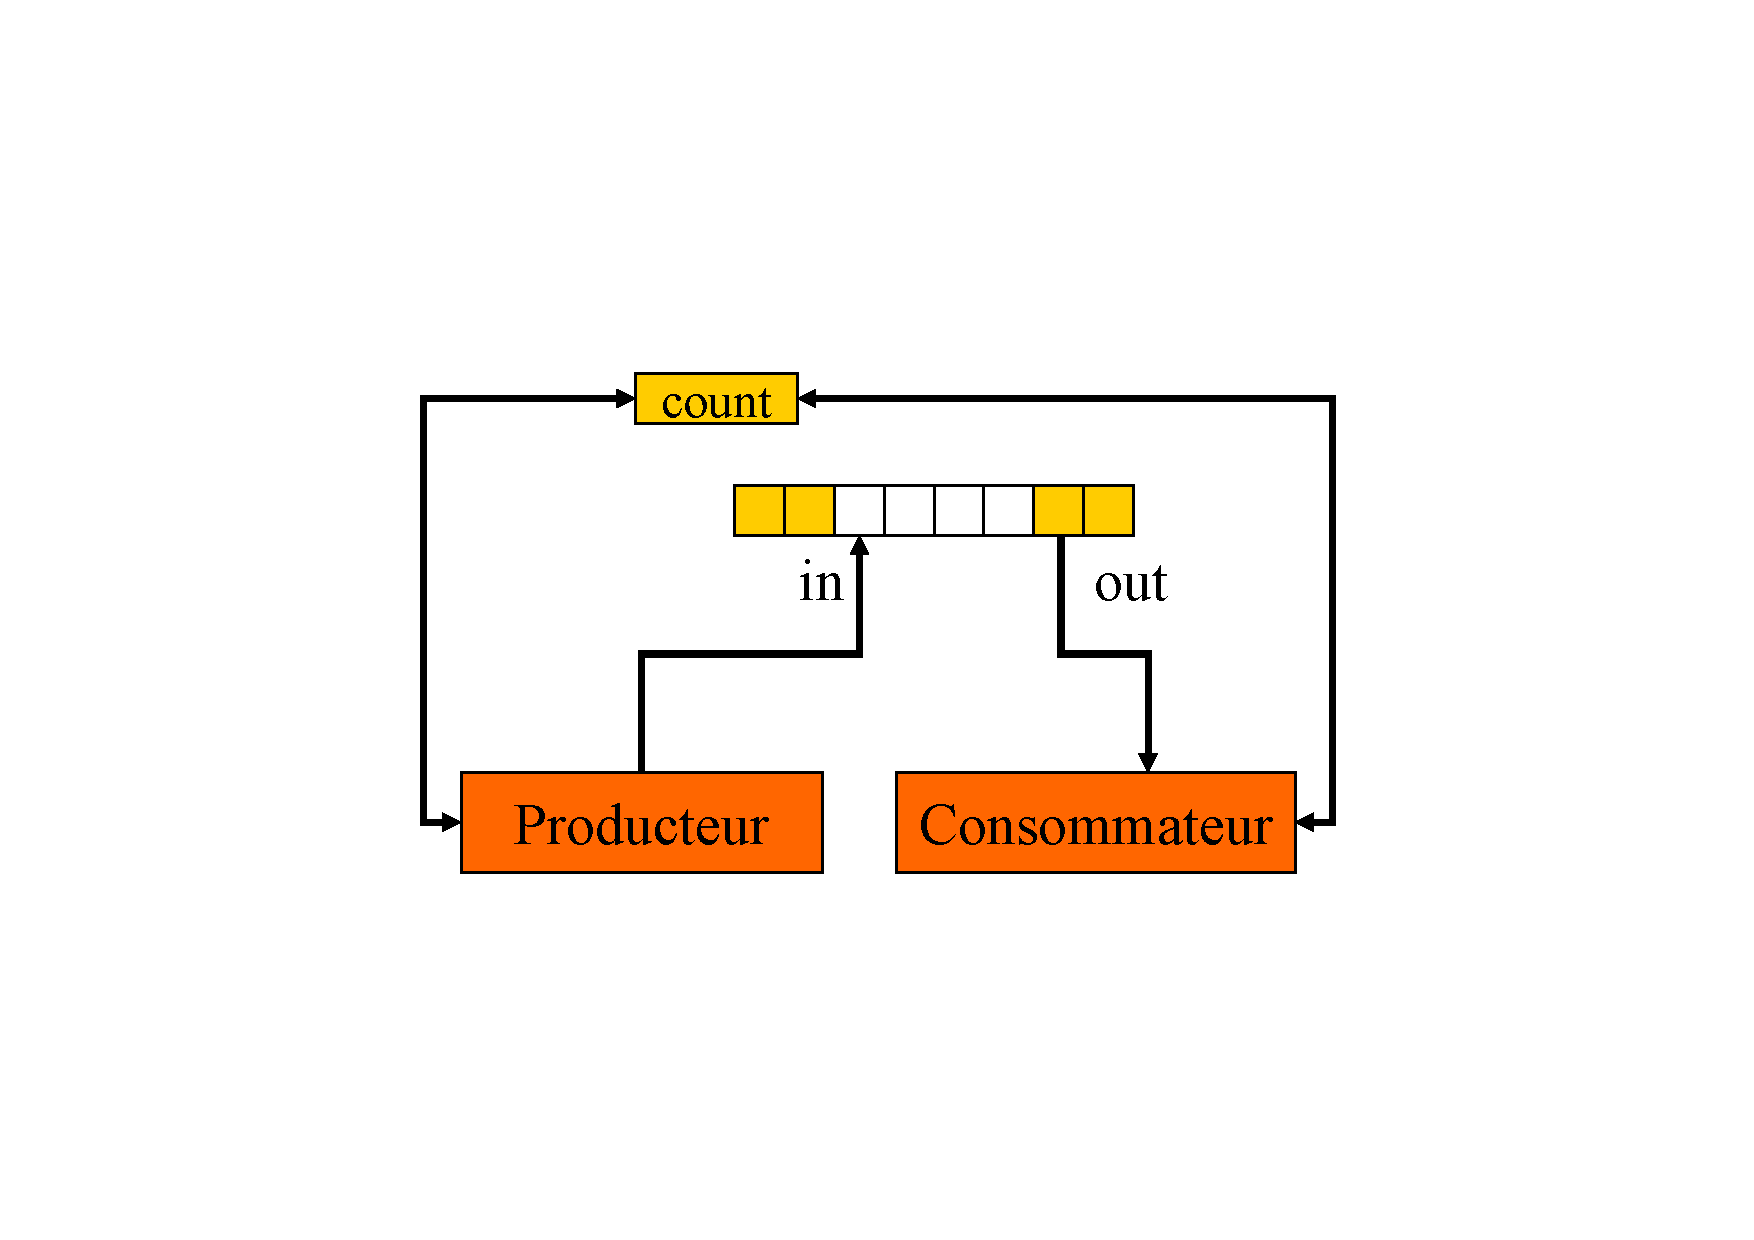
\includegraphics[width=5cm]{../illustration/prod_consom_tampon.pdf}
\end{center}
\end{frame}

\begin{frame}
\frametitle{Problème du tampon borné}
\begin{itemize}
\item Trois sémaphores :
\begin{itemize}
\item[Libre] Compte les emplacements libres
\begin{center}\textit{Initialisé à la capacité du tampon}\end{center}
\item[Occupé] Compte les emplacements occupés
\begin{center}\textit{Initialisé à zéro}\end{center}
\item[Mutex] Protection des sections critiques de modification du tampon
\begin{center}\textit{Initialisé à un}\end{center}
\end{itemize}
\end{itemize}
\end{frame}

\begin{frame}
\frametitle{Problème du tampon borné}
\begin{columns}
\column{0.45\textwidth}
Ajout d’un élément :
\begin{scriptsize}\verbatiminput{include/tb_ajout.c}\end{scriptsize}
\column{0.45\textwidth}
Extraction d’un élément :
\begin{scriptsize}\verbatiminput{include/tb_retire.c}\end{scriptsize}
\end{columns}
\end{frame}

\begin{frame}
\frametitle{Problème du tampon borné}
\framesubtitle{Exemple en C}
\begin{multicols}{2}
\begin{scriptsize}\verbatiminput{include/tb_exemple.c}\end{scriptsize}
\end{multicols}
\end{frame}


\begin{frame}
\frametitle{Problème des lecteurs/rédacteurs}
\begin{itemize}
\item Base de données \textbf{partagée} :
\begin{itemize}
\item [Rédacteurs] Mettent à jour la base
\item [Lecteurs] Consultent la base
\end{itemize}
\item \textbf{Rédaction exclusive} de tout autre accès :
\begin{itemize}
\item Un rédacteur ne peut modifier la base que si aucun lecteur n’y accède et aucun autre rédacteur ne la modifie
\item Accès exclusif à la base pour les rédacteurs
\end{itemize}
\end{itemize}
\end{frame}

\begin{frame}
\frametitle{Problème des lecteurs/rédacteurs}
\begin{itemize}
\item <1-> 1$^{er}$ problème
\begin{itemize}
\item Aucun lecteur ne reste en attente pour l’accès à la base de données, sauf lorsqu’un rédacteur la modifie
\item Risque de \textbf{famine} pour les \textbf{rédacteurs}
\end{itemize}
\item <2-> 2$^{eme}$ problème
\begin{itemize}
\item Quand il est prêt, un rédacteur effectue ses modifications dès que possible
\item Risque de \textbf{famine} pour les \textbf{lecteurs}
\end{itemize}
\end{itemize}
\end{frame}

\begin{frame}
\frametitle{Problème des lecteurs/rédacteurs}
\begin{itemize}
\item Variables :
\begin{itemize}
\item Base de données : \texttt{base}
\item Compteur de lecteur : \texttt{nb\_lecteur}
\end{itemize}
\item Méthodes :
\begin{itemize}
\item \texttt{debutLecture()}
\item \texttt{finLecture()}
\item \texttt{debutEcriture()}
\item \texttt{finEcriture()}
\end{itemize}
\end{itemize}
\end{frame}

\begin{frame}
\frametitle{Problème des lecteurs/rédacteurs}
\begin{columns}
\column{0.45\textwidth}
\begin{scriptsize}\verbatiminput{include/tb_debutLecture.java}\end{scriptsize}
\column{0.45\textwidth}
\begin{scriptsize}\verbatiminput{include/tb_finLecture.java}\end{scriptsize}
\end{columns}
\end{frame}


\begin{frame}
\frametitle{Problème du dîner des philosophes}
\begin{columns}
\column{0.45\textwidth}
\begin{itemize}
\item 5 philosophes
\item 5 fourchettes
\item 2 activités :
\begin{itemize}
\item Penser
\item Manger
\end{itemize}
\end{itemize}
\column{0.45\textwidth}

\includegraphics[width=5cm]{../illustration/diner_philosophes.pdf}
\end{columns}
\begin{center}
Pour manger, un philosophe doit prendre successivement deux fourchettes
\end{center}
\end{frame}

\begin{frame}
\frametitle{Implémentation logicielle}
\framesubtitle{Programmation du comportement du philosophe(i)}
\begin{scriptsize}
\verbatiminput{include/comport_philo.java}
\end{scriptsize}
\end{frame}

\begin{frame}
\frametitle{Problème du dîner des philosophes}
\begin{center}

\includegraphics[height=.9\textheight]{../illustration/diner_philosophes_ib.pdf}
\end{center}
\end{frame}

\begin{frame}
\frametitle{Problème du dîner des philosophes}
\framesubtitle{Propositions de solutions pour éviter les interblocages}
\begin{itemize}
\item <1-> N’accepter que quatre philosophes autour de la table
\item <2-> Ajouter une fourchette
\item <3-> Ne prendre les fourchettes que si les deux sont libres
\begin{itemize}
\item Au sein d’une section critique
\item ...avec condition de sortie si une des fourchettes n'est pas disponible
\end{itemize}
\item <4-> Utiliser une solution asymétrique
\begin{itemize}
\item Les philosophes pairs prennent d’abord leur fourchette gauche
\item ...les impaires font le contraire
\end{itemize}
\end{itemize}
\end{frame}

\section{Lutte contre les interblocages}

\begin{frame}
\frametitle{Interblocage : définition}
\begin{itemize}
\item Plusieurs processus en concurrence
\item Pour accéder à un nombre limité de ressources
\item Interblocage :
\begin{itemize}
\item Processus en attente d’une ressource bloquée par un autre processus en attente elle aussi
\item Attente mutuelle - Étreinte fatale ou dead lock
\item Dégradation des performances
\end{itemize}
\end{itemize}
\end{frame}

\subsection{Conditions nécessaires}
\begin{frame}
\frametitle{Conditions nécessaires à un interblocage}
\begin{itemize}
\item Conjonction de quatre circonstances :
\begin{itemize}
\item \textbf{Exclusion mutuelle} :
\begin{itemize}
\item Au moins une ressource non partageable
\end{itemize}
\item \textbf{Détention et attente} :
\begin{itemize}
\item Au moins un processus qui possède une ressource et qui en attend une autre
\end{itemize}
\item \textbf{Pas de préemption} :
\begin{itemize}
\item Ressources devant être libérées volontairement
\end{itemize}
\item \textbf{Attente circulaire}
\end{itemize}
\end{itemize}
\end{frame}

\subsection{Action sur "exclusion mutuelle"}

\begin{frame}
\frametitle{Action sur "exclusion mutuelle"}
\begin{itemize}
\item Ressource utilisable exclusivement par un processus et un seul
\begin{itemize}
\item Lorsque la ressource est utilisée par un processus, elle n’est plus disponible pour les autres
\item Attente de libération
\end{itemize}
\item Son partage donnerait des résultats incohérents
\end{itemize}
\end{frame}


\subsection{Action sur "détention et attente"}
\begin{frame}
\frametitle{Action sur "détention et attente"}
\begin{itemize}
\item Première solution :
\begin{itemize}
\item Chaque processus ne peut progresser que s’il obtient des ressources,
\item Il requière ses ressources dynamiquement, par demandes successives au cours de son exécution,
\item Il attend donc les ressources de sa dernière requête avant de poursuivre son déroulement.
\end{itemize}
\item Autre solution :
\begin{itemize}
\item Timeout sur la demande de ressource supplémentaire
\item Évite la détention et attente infinie 
\end{itemize}
\end{itemize}

\end{frame}

\subsection{Action sur "pas de préemption"}

\begin{frame}
\frametitle{Action sur "pas de préemption"}
\begin{itemize}
\item Les ressources déjà allouées restent nécessaires aux processus qui les ont reçu
\item Ces ressources ne peuvent pas être réquisitionnées, par le système ou un autre processus
\item On ne peut pas retirer d'autorité une ressource allouée
\end{itemize}
\end{frame}

\subsection{Action sur "attente circulaire"}

\begin{frame}
\frametitle{Action sur "attente circulaire"}
\begin{itemize}
\item Processus en attente de ressources allouées à d’autres processus
\item Il s’est formé une attente circulaire entre les processus
\item Exemple :
\begin{itemize}
\item Le processus A attend des ressources détenues par B, qui lui même attend des ressources détenues par A
\end{itemize}
\end{itemize}
\end{frame}

\begin{frame}
\frametitle{Graphe d’allocation de ressources}
\begin{itemize}
\item <1-> Graphe orienté
\item <2-> Sommets :
\begin{itemize}
\item Processus du système (cercles)
\item Ressources du système (carrés)
\end{itemize}
\item <3-> Arêtes orientées :
\begin{itemize}
\item Détention de ressources
\begin{itemize}
\item ressource $\to$ processus
\end{itemize}
\item Demande de ressource
\begin{itemize}
\item processus $\to$ ressource
\end{itemize}
\end{itemize}
\end{itemize}
\end{frame}

\begin{frame}
\frametitle{Graphe d’allocation de ressources}
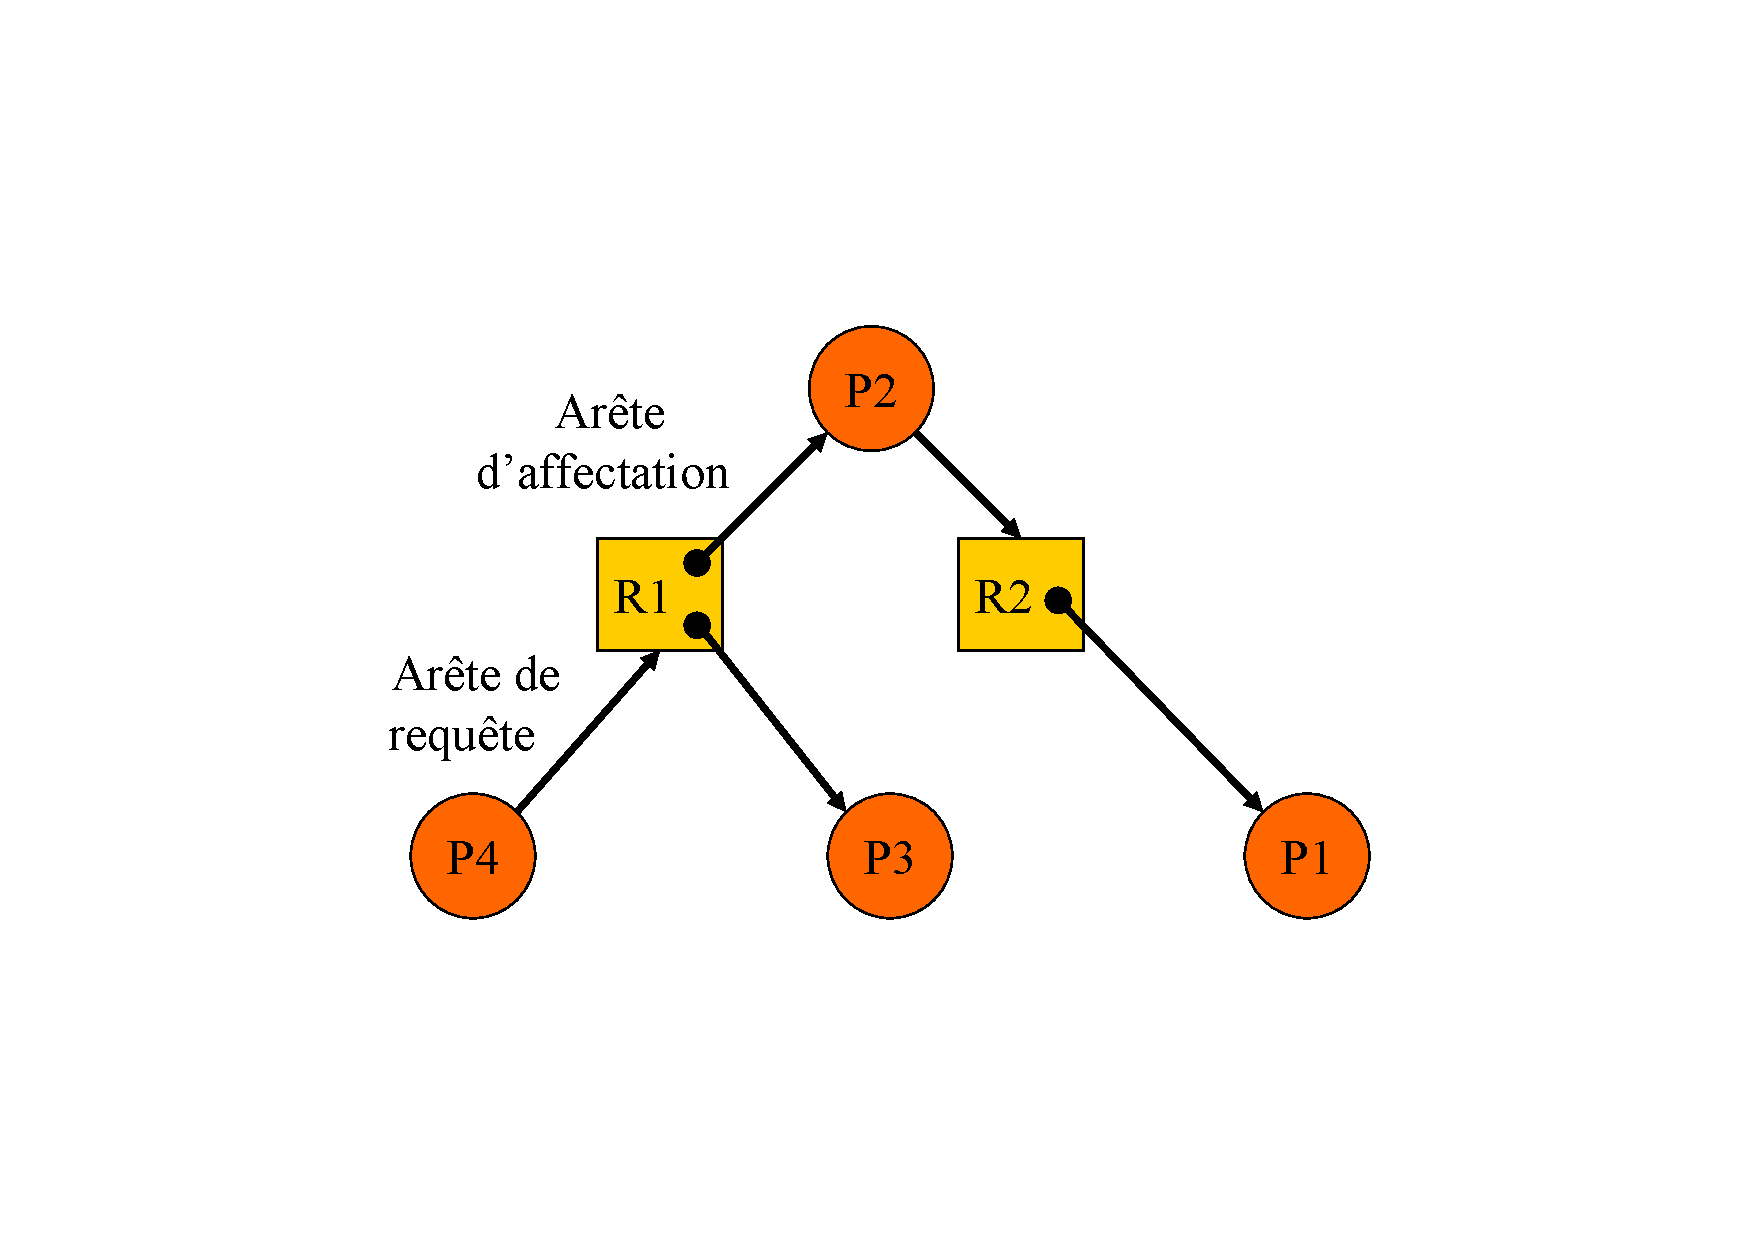
\includegraphics[width=.8\textwidth]{../illustration/graphe_alloc_ressource.pdf}
\end{frame}

\begin{frame}
\frametitle{Graphe d’allocation de ressources}
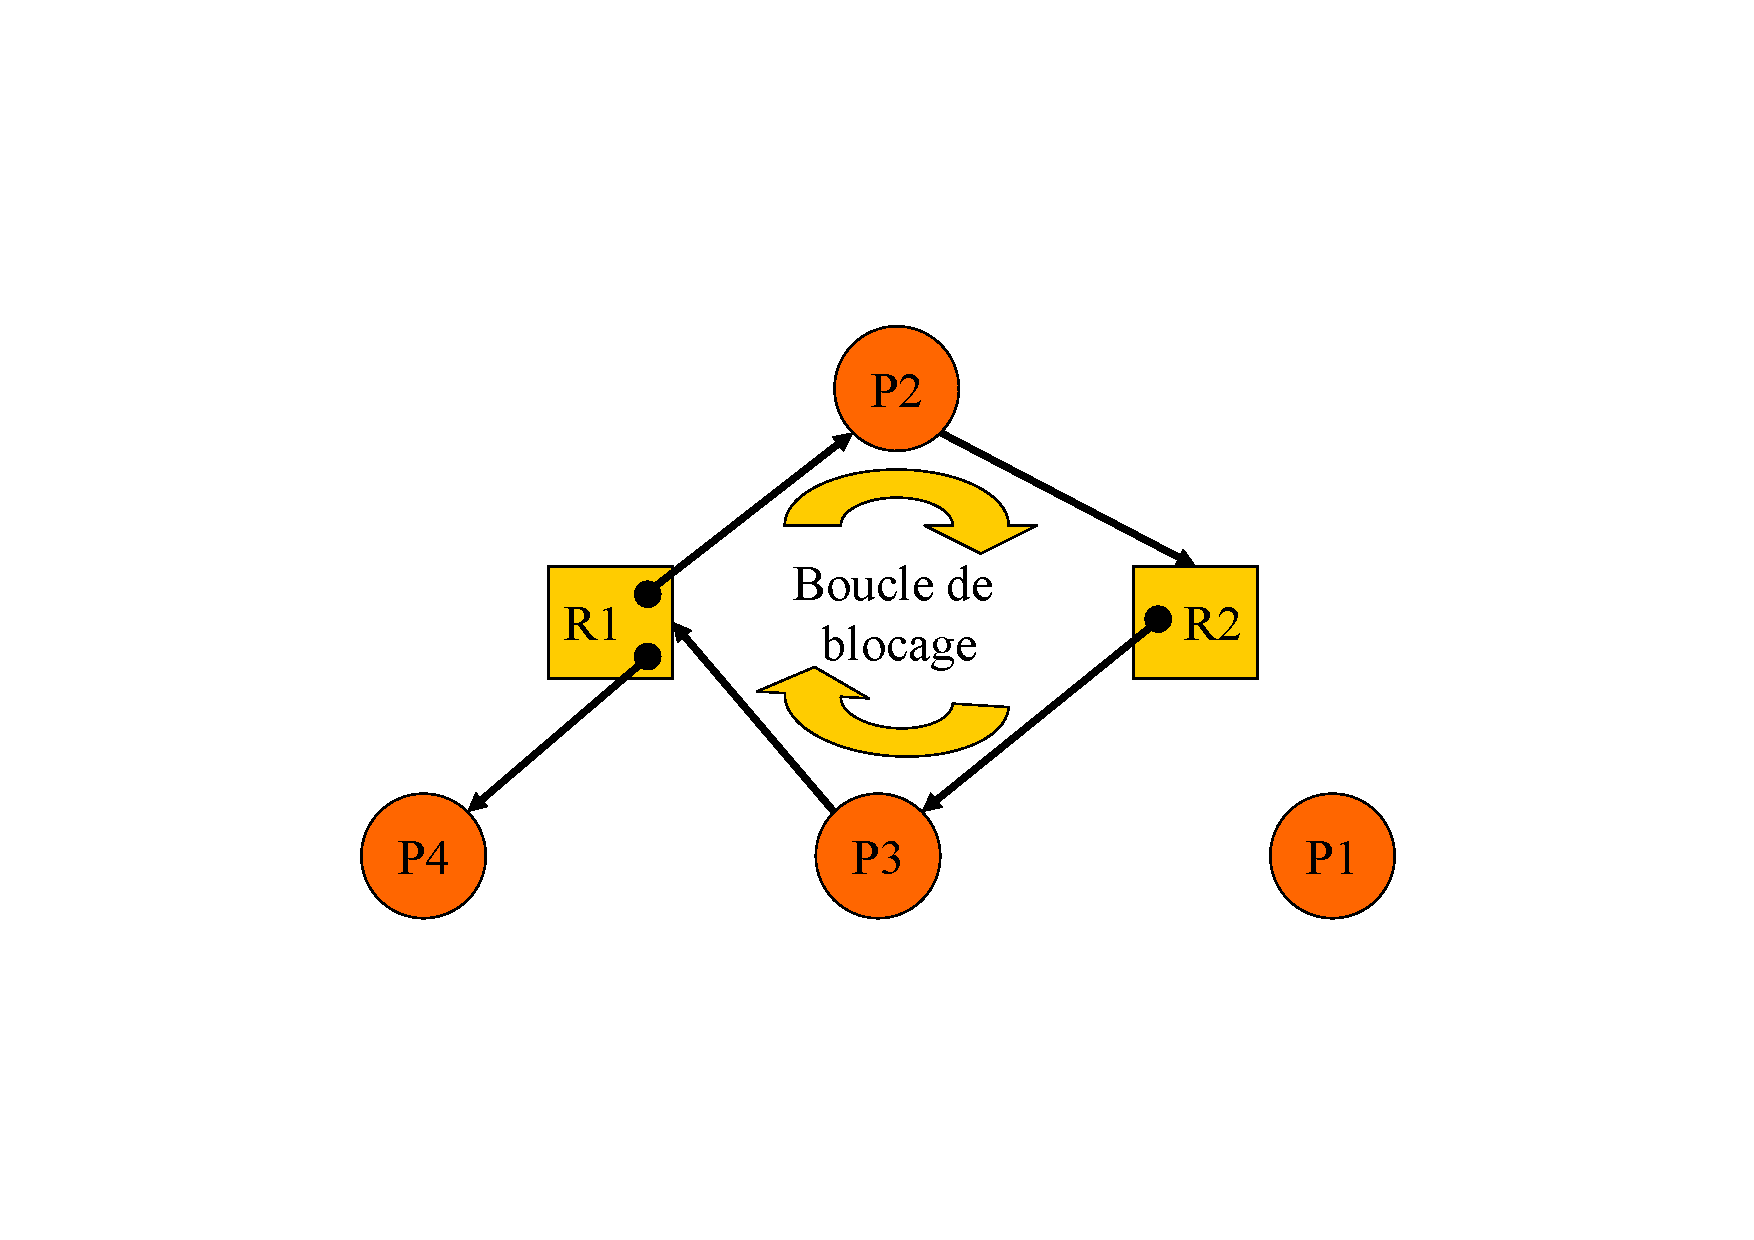
\includegraphics[width=.8\textwidth]{../illustration/graphe_alloc_ressource_ib.pdf}
\end{frame}

\begin{frame}
\frametitle{Cycle et interblocage}
\begin{itemize}
\item Si chaque ressource est unique :
\begin{itemize}
\item Processus en interblocage
\item Condition nécessaire et suffisante
\end{itemize}
\item Si chaque ressource possède plusieurs instances :
\begin{itemize}
\item Pas forcement d’interblocage
\item Condition nécessaire mais pas suffisante
\end{itemize}
\end{itemize}
\end{frame}

\begin{frame}
\frametitle{Exemple de cycle sans interblocage}
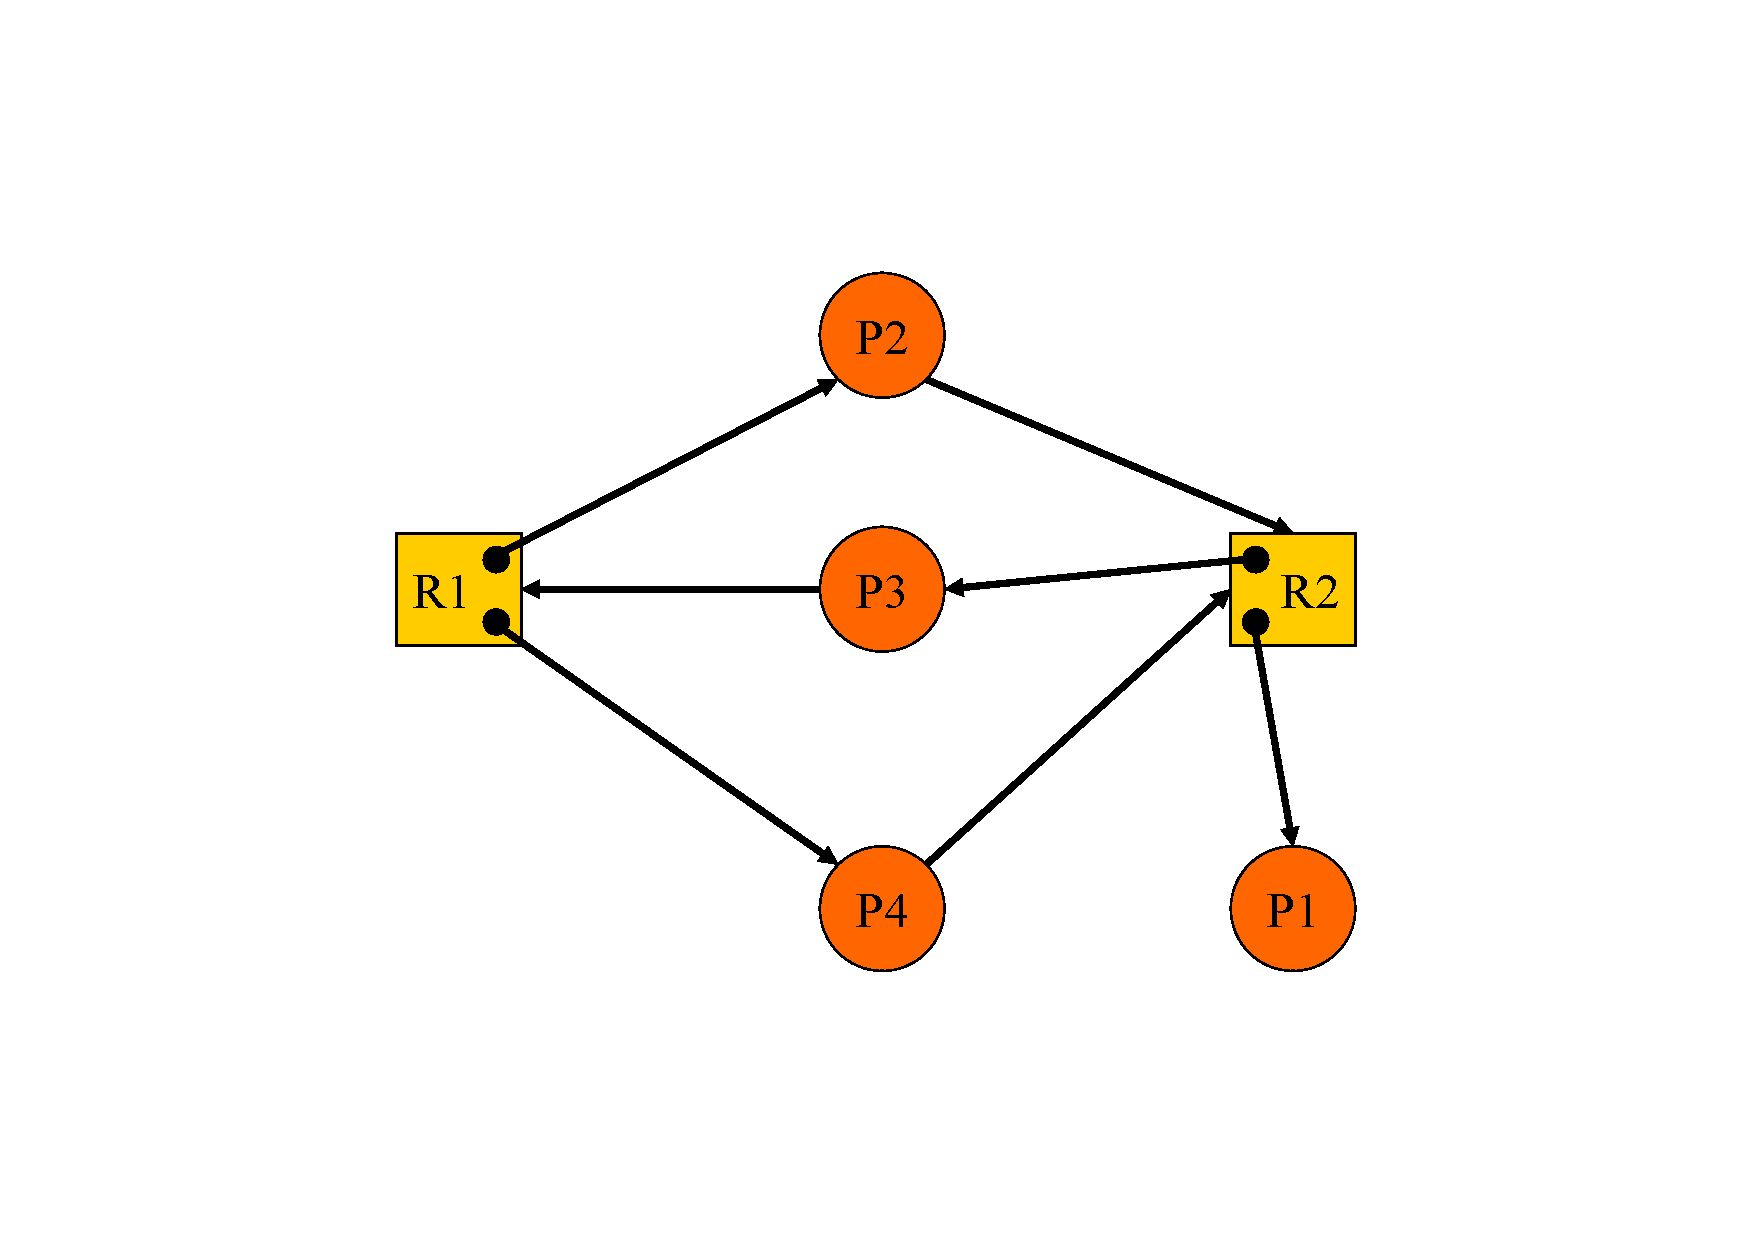
\includegraphics[width=.8\textwidth]{../illustration/graphe_alloc_ressource_cycle_sans_ib.pdf}
\end{frame}

\begin{frame}
\frametitle{Méthodes de lutte contre l’interblocage}
\begin{itemize}
\item \textbf{Détection guérison}
\begin{itemize}
\item Mécanismes d’identification et de sortie d’un état d’interblocage
\end{itemize}
\item \textbf{Protocole de prévention}
\begin{itemize}
\item Évite l’entrée en interblocage
\begin{itemize}
\item \textbf{Prévention statique} : étude conditions d’apparition
\item \textbf{Prévention dynamique} : allocation de ressources
\end{itemize}
\end{itemize}
\item \textbf{Ignorer le problème}
\begin{itemize}
\item Prétendre que le système n’entre jamais en interblocage
\includegraphics[width=2cm]{../illustration/autruche.jpg}
\end{itemize}
\end{itemize}
\end{frame}

\begin{frame}
\frametitle{Principes de la \textbf{détection guérison}}
\begin{itemize}
\item <1-> [détection] Algorithme de détection des interblocages
\begin{itemize}
\item Ausculte régulièrement le système
\item Identifie les situations d’interblocage
\begin{itemize}
\item blocages + attentes circulaires
\end{itemize}
\end{itemize}
\item <2-> [guérison] Algorithme pour mettre fin aux interblocages détectés
\begin{itemize}
\item Supprime au moins une des conditions nécessaires à l’interblocage
\item Recherche de la solution la moins coûteuse
\end{itemize}
\end{itemize}
\end{frame}

\begin{frame}
\frametitle{Détection guérison : détection d’interblocage}
\begin{itemize}
\item Utilisation d’un \textbf{graphe d’attente} :
\begin{itemize}
\item Toutes les ressources n’ont qu’une instance
\item Obtenu à partir du graphe d’allocation
\item Retirer les nœuds de type ressource
\item Réunir les arcs par transitivité
\end{itemize}
\item Recherche de cycle
\item Algorithme lancé régulièrement
\end{itemize}
\end{frame}

\begin{frame}
\frametitle{Exemple de graphe d’attente}
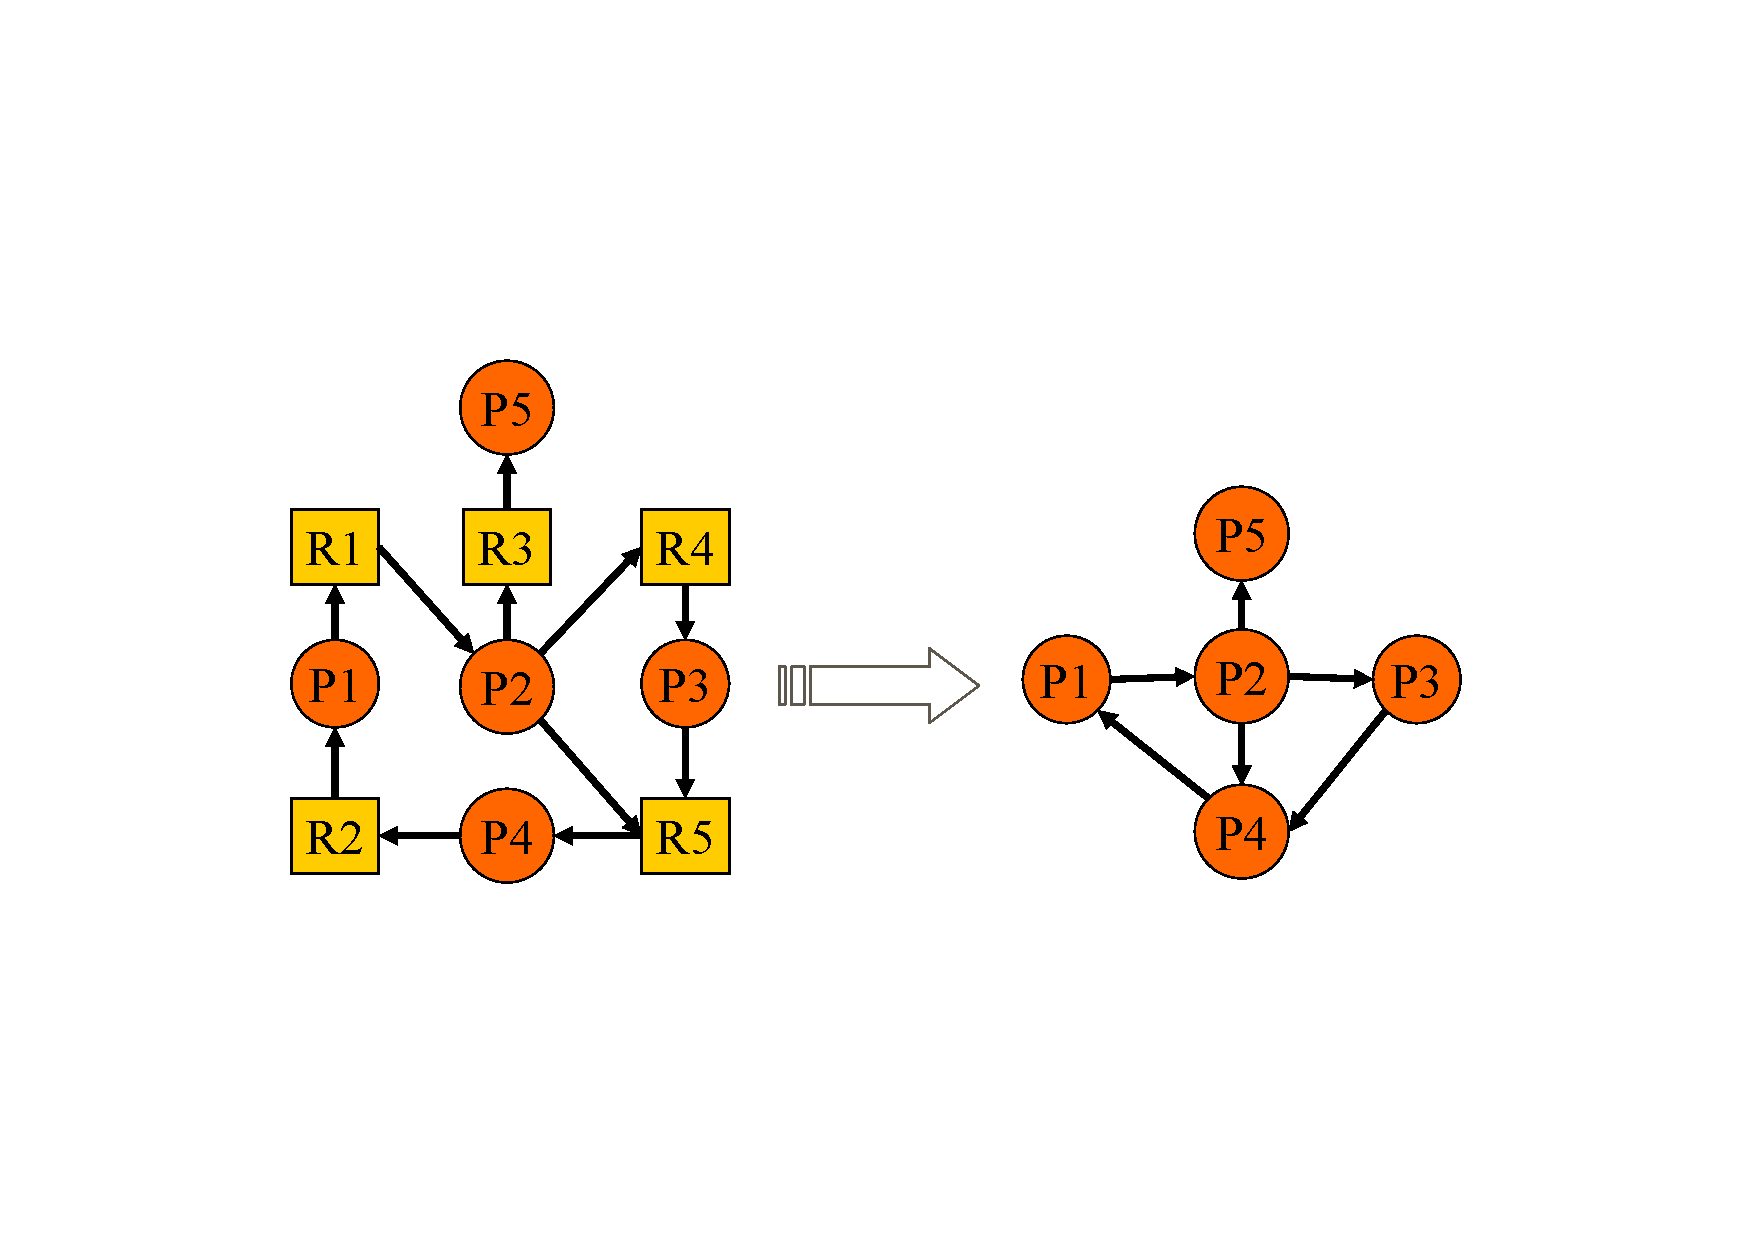
\includegraphics[width=.9\textwidth]{../illustration/gar2ga.pdf}
\end{frame}

\begin{frame}
\frametitle{Correction d’interblocage}
\begin{itemize}
\item Plusieurs alternatives en cas de détection d’interblocage :
\begin{itemize}
\item Informer un opérateur pour correction manuelle
\item Corriger automatiquement le problème
\end{itemize}
\item Correction d’interblocage :
\begin{itemize}
\item Arrêt d’un ou plusieurs processus
\item Réquisition de ressources
\end{itemize}
\item Toujours violent
\end{itemize}
\end{frame}

\begin{frame}
\frametitle{Terminaison de processus}
Deux méthodes :
\begin{columns}
\column{0.45\textwidth}
\begin{block}<1->{Arrêter tous les processus en interblocage}
\begin{itemize}
\item Pertes élevées
\item perte d’informations, de résultats qu’il faudra, au mieux, de nouveau calculer
\end{itemize}
\end{block}
\column{0.45\textwidth}
\begin{block}<2->{Arrêter les processus un par un}
\begin{itemize}
\item Lancement de l’algorithme de détection des interblocages après chaque arrêt
\item jusqu’à la disparition de l’interblocage
\item Coûteux en temps de calcul
\end{itemize}
\end{block}
\end{columns}
\end{frame}

\begin{frame}
\frametitle{Terminaison de processus}
\begin{itemize}
\item Arrêt de processus :
\begin{itemize}
\item Risque de laisser les ressources dans un état inconsistant
\begin{itemize}
\item Fichier en cours de modification
\item Verrou non libéré
\end{itemize}
\item Ordre de terminaison :
\begin{itemize}
\item Commencer par les moins coûteux (subjectif)
\end{itemize}
\end{itemize}
\end{itemize}
\end{frame}

\begin{frame}
\frametitle{Choix d’une victime}
\begin{itemize}
\item <1->Le coût de terminaison du processus victime doit être minimal
\item <2->Facteur de coût :
\begin{itemize}
\item Nombre de ressources allouées
\item Temps de calcul passé / restant
\item Interactif ou non
\item Priorité du processus
\item Occupation mémoire
\end{itemize}
\item <3->Variable en fonction de la destination du système
\end{itemize}
\end{frame}

\begin{frame}
\frametitle{Préemption de ressources}
\begin{itemize}
\item <1->Préemption de ressources et allocation à d’autres processus jusqu’à disparition de l’interblocage
\item <2->Problèmes :
\begin{itemize}
\item Choix de la ressource à réquisitionner (victime)
\item Devenir du processus qui s’est fait préempter une ressource ?
\item Famine
\end{itemize}
\end{itemize}
\end{frame}

\begin{frame}
\frametitle{Devenir du processus}
\framesubtitle{Que se passera-t-il après préemption d’une ressource ?}
\begin{itemize}
\item <1->Le processus préempté ne peut pas reprendre son exécution normalement
\item <2->Ramener le processus dans un état sain
\begin{itemize}
\item Plus simple : reprendre l’exécution à son origine
\item Plus fin : nécessite au système de maintenir des informations sur l’état des processus (points de reprise)
\end{itemize}
\item <3->Dans l'idéal, la préemption de ressource devrait être préparée à l'avance pour permettre :
\begin{itemize}
\item La poursuite du traitement
\item La restitution d'une ressource consistante
\end{itemize}
\end{itemize}
\end{frame}

\begin{frame}
\frametitle{Risque de famine}
\begin{itemize}
\item <1->Risque de toujours préempter les ressources du même processus
\begin{itemize}
\item Surtout si l’on se base sur des notions de coût
\end{itemize}
\item <2-> Le processus concerné peut alors se retrouver dans un état de famine
\begin{itemize}
\item Victime idéale
\end{itemize}
\item <3->Nécessiter de tenir compte du nombre de préemption subit par le processus dans le calcul de coût
\begin{itemize}
\item Enchérissement des précédentes victimes
\end{itemize}
\end{itemize}
\end{frame}

\begin{frame}
\frametitle{Principe du protocole de prévention}
\begin{itemize}
\item S’assurer qu’au moins une des quatre conditions nécessaires n’est pas vérifiée :
\begin{itemize}
\item Exclusion mutuelle
\item Détention et attente
\item Pas de préemption
\item Attente circulaire
\end{itemize}
\item Méthode préventive
\item Évite la destruction de processus
\begin{itemize}
\item Violente et coûteuse
\end{itemize}
\end{itemize}
\end{frame}

\begin{frame}
\frametitle{Les états du système}
\begin{itemize}
\item <1-> \textbf{État sain}
\begin{itemize}
\item Le système n'est pas en interblocage à ou n'est pas sur la voie de l'être
\item Risque potentiel de conduire le système vers un interblocage
\end{itemize}
\item <2-> \textbf{État fiable}
\begin{itemize}
\item Aucun risque de conduire le système vers un interblocage
\end{itemize}
\item <3-> Un système fiable est forcement sain
\end{itemize}
\end{frame}

\begin{frame}
\frametitle{Protocoles utilisés}
\begin{itemize}
\item Protocole de prévention statique
\item Protocole de prévention dynamique
\item Prévention destructive par estampilles
\end{itemize}
\end{frame}

\begin{frame}
\frametitle{Protocole de prévention statique}
\begin{itemize}
\item Politique d’allocation de ressources permettant d’éviter l’interblocage :
\begin{itemize}
\item Tout processus doit demander les ressources dont il à besoin en une fois, au début de son exécution
\item Il les recevra en bloc, même s’il ne les utilise pas immédiatement
\item Possibilité de mutualiser demandes par classe
\end{itemize}
\end{itemize}
\end{frame}

\begin{frame}
\frametitle{Protocole de prévention dynamique}
\begin{itemize}
\item Prévention dynamique (ou évitement) par attente et retard de service
\item But :
\begin{itemize}
\item Identifier les processus à risque
\item Les bloquer avant qu’ils ne provoquent un interblocage
\item Ne les débloquer que lorsqu’il n’y a plus de risque d’interblocage
\end{itemize}
\end{itemize}
\end{frame}

\begin{frame}
\frametitle{Protocole de prévention dynamique}
\begin{itemize}
\item <1-> Estimer le comportement potentiel des processus
\begin{itemize}
\item annonce préalable des ressources utilisables
\item Annonce explicite et contractuelle
\item Évaluation de la possibilité de répondre à toutes les demandes futures, même maximales
\end{itemize}
\item <2-> S’il y a risque d’interblocage, le système bloque le processus demandeur
\end{itemize}
\end{frame}

\begin{frame}
\frametitle{Protocole de prévention dynamique}
\begin{itemize}
\item L'allocateur oblige le système à \textbf{rester} dans des \textbf{états fiables}, à partir desquels le système ne peut jamais évoluer vers un interblocage
\item Possibilité de \textbf{refus de service}, même si l'allocateur dispose des ressources pour satisfaire la demande instantanée.
\end{itemize}
\end{frame}

\begin{frame}
\frametitle{Protocole de prévention dynamique}
\begin{itemize}
\item Risque de sous utilisation des ressources si les annonces sont inexactes.
\item Il n'est pas toujours possible de connaître toutes les ressources qu'un processus va utiliser :
\begin{itemize}
\item Estimer un majorant conduirait à recenser toutes les ressources,
\item Exemple : Base de données
\end{itemize}
\end{itemize}
\end{frame}

\begin{frame}
\frametitle{Prévention destructive par estampilles}
\begin{itemize}
\item Applicable aux systèmes transactionnels
\item Principe :
\begin{itemize}
\item Dater les transactions en leur associant une estampille et utiliser l'ordre total ainsi obtenu pour régler le conflit d'accès aux ressources
\end{itemize}
\item La transaction abandonnée redémarre avec son ancienne estampille, ce qui prévient la famine
\begin{itemize}
\item Possibilité de point de reprise
\end{itemize}
\end{itemize}
\end{frame}

\begin{frame}
\frametitle{Prévention destructive par estampilles}
\begin{itemize}
\item Adaptée quand l'identité des ressources accédées n'est pas connue au début de la transaction et qu'elle varie en cours d’exécution.
\item Méthode pessimiste :
\begin{itemize}
\item La transaction perdante est abandonnée, même si elle n'utilise aucune ressource.
\end{itemize}
\end{itemize}
\end{frame}

\begin{frame}
\frametitle{Principes de la prévention d’interblocage}
\begin{itemize}
\item Éviter la conjonction des conditions nécessaires à la survenue d’un interblocage :
\begin{itemize}
\item Exclusion mutuelle
\item Détention et attente
\item Pas de préemption
\item Attente circulaire
\end{itemize}
\end{itemize}
\end{frame}

\begin{frame}
\frametitle{Limiter les besoins d’exclusion mutuelle}
\begin{itemize}
\item Nécessaire pour l’utilisation de ressources non partageables
\item Pour les ressources partageables :
\begin{itemize}
\item Pas d’accès exclusif nécessaire
\item Jamais d’attente sur une ressource partageable
\end{itemize}
\item Solution :
\begin{itemize}
\item Rendre un maximum de ressources partageables
\end{itemize}
\end{itemize}
\end{frame}

\begin{frame}
\frametitle{Limiter les besoins d’exclusion mutuelle}
\begin{itemize}
\item Sérialiser les requêtes portant sur une ressource
\item Par exemple :
\begin{itemize}
\item Utilisation d’un spool d’impression pour les imprimantes
\item Traitement en série des demandes d’impression par un démon
\item Le périphérique, bien que non partageable, ne semble jamais occupé pour les processus
\end{itemize}
\end{itemize}
\end{frame}

\begin{frame}
\frametitle{Éviter la détention et attente}
\begin{itemize}
\item S’assurer qu’un processus qui demande une ressource non partageable n’en détient pas une autre
\item Possibilités :
\begin{itemize}
\item Imposer la demande de toutes les ressources avant utilisation
\item Accepter uniquement les demandes de ressource provenant de processus n’en détenant aucune (libération préalable)
\end{itemize}
\end{itemize}
\end{frame}

\begin{frame}
\frametitle{Éviter la détention et attente}
\begin{itemize}
\item Exemple :
Copie de données d’une bande vers un disque
Tri du fichier
Impression
\end{itemize}
\begin{columns}
\column{0.45\textwidth}
\begin{block}<1->{Méthode 1}
\begin{itemize}
\item Demande bande, disque et imprimante
\item Bloque l’imprimante pendant tout le traitement, même s’il ne l’utilise qu’à la fin
\end{itemize}
\end{block}
\column{0.45\textwidth}
\begin{block}<2->{Méthode 2}
\begin{itemize}
\item Demande bande et disque
\item Libération des deux
\item Demande disque et imprimante
\end{itemize}
\end{block}
\end{columns}
\end{frame}

\begin{frame}
\frametitle{Éviter la détention et attente}
\begin{block}{Inconvénients}
\begin{itemize}
\item Utilisation des ressources peu efficace
\begin{itemize}
\item ressources bloquées et inutilisées
\end{itemize}
\item Possibilité de famine
\item Très contraignant à réaliser
\begin{itemize}
\item allocation est souvent dynamique
\end{itemize}
\end{itemize}
\end{block}
\end{frame}

\begin{frame}
\frametitle{Éviter la détention et attente}
\begin{block}{Solution}
\begin{itemize}
\item Identifier des classes de ressource
\begin{itemize}
\item Les unités de bande
\item Les imprimantes...
\end{itemize}
\item Imposer un ordre strict d’allocation de ressource par classe
\end{itemize}
\end{block}

Exemple :
\begin{itemize}
\item On ne peut demander une unité de bande si on détient déjà une imprimante
\end{itemize}
\end{frame}

\begin{frame}
\frametitle{Permettre la préemption}
\begin{itemize}
\item Les processus en interblocage ne peuvent pas rendre les ressources qu’ils possèdent
\item On ne peut pas retirer d'autorité une ressource allouée
\end{itemize}
\begin{block}{Solution}
Permettre au système de réquisitionner des ressources bloqués par des processus
\end{block}
\end{frame}

\begin{frame}
\frametitle{Permettre la préemption}
\begin{itemize}
\item Si un processus demande des ressources non disponibles immédiatement :
\begin{itemize}
\item <1->Libération des ressources détenues si elles sont demandées par d’autres processus
\item <2->Ajout de ces ressources à la liste des ressources attendues
\item <3->Préemption éventuelle de ressources détenues par des processus en attente
\item <4->Redémarrage du processus lorsqu’il a obtenu toutes les ressources demandées
\end{itemize}
\end{itemize}
\end{frame}

\begin{frame}
\frametitle{Permettre la préemption}
Déroulement d'une demande de ressource :
\begin{itemize}
\item <1->Si la ressource est disponible
\begin{itemize}\item Allocation des ressources au processus\end{itemize}
\item <2->Si la ressource n'est pas disponible
\begin{itemize}
\item <3->Si elle est allouée à d’autres processus bloqués :
\begin{itemize}\item \textbf{préemption} des ressources\end{itemize}
\item <4->Sinon :
\begin{itemize}\item \textbf{mise en attente} du processus demandeur\end{itemize}
\end{itemize}
\end{itemize}
\end{frame}

\begin{frame}
\frametitle{Permettre la préemption}
\begin{itemize}
\item Pas raisonnable pour la plupart des ressources sans dégrader profondément le fonctionnement du système
\item Envisageable pour certaines ressources dont le contexte peut être facilement sauvegardé et restauré
\end{itemize}
\end{frame}

\begin{frame}
\frametitle{Éviter l’attente circulaire}
Éviter les boucles dans le graphe d’allocation de ressources
\begin{block}{Solution}
\begin{itemize}
\item Attribuer un numéro d’ordre à chaque type de ressource
\item Imposer l’allocation des ressources dans l’ordre croissant des numéros
\begin{itemize}
\item Demande d’une ressource d’ordre n est rejetée si le processus possède déjà une ressource d’ordre n+1
\end{itemize}
\end{itemize}
\end{block}
\end{frame}

\begin{frame}
\frametitle{Éviter l’attente circulaire}
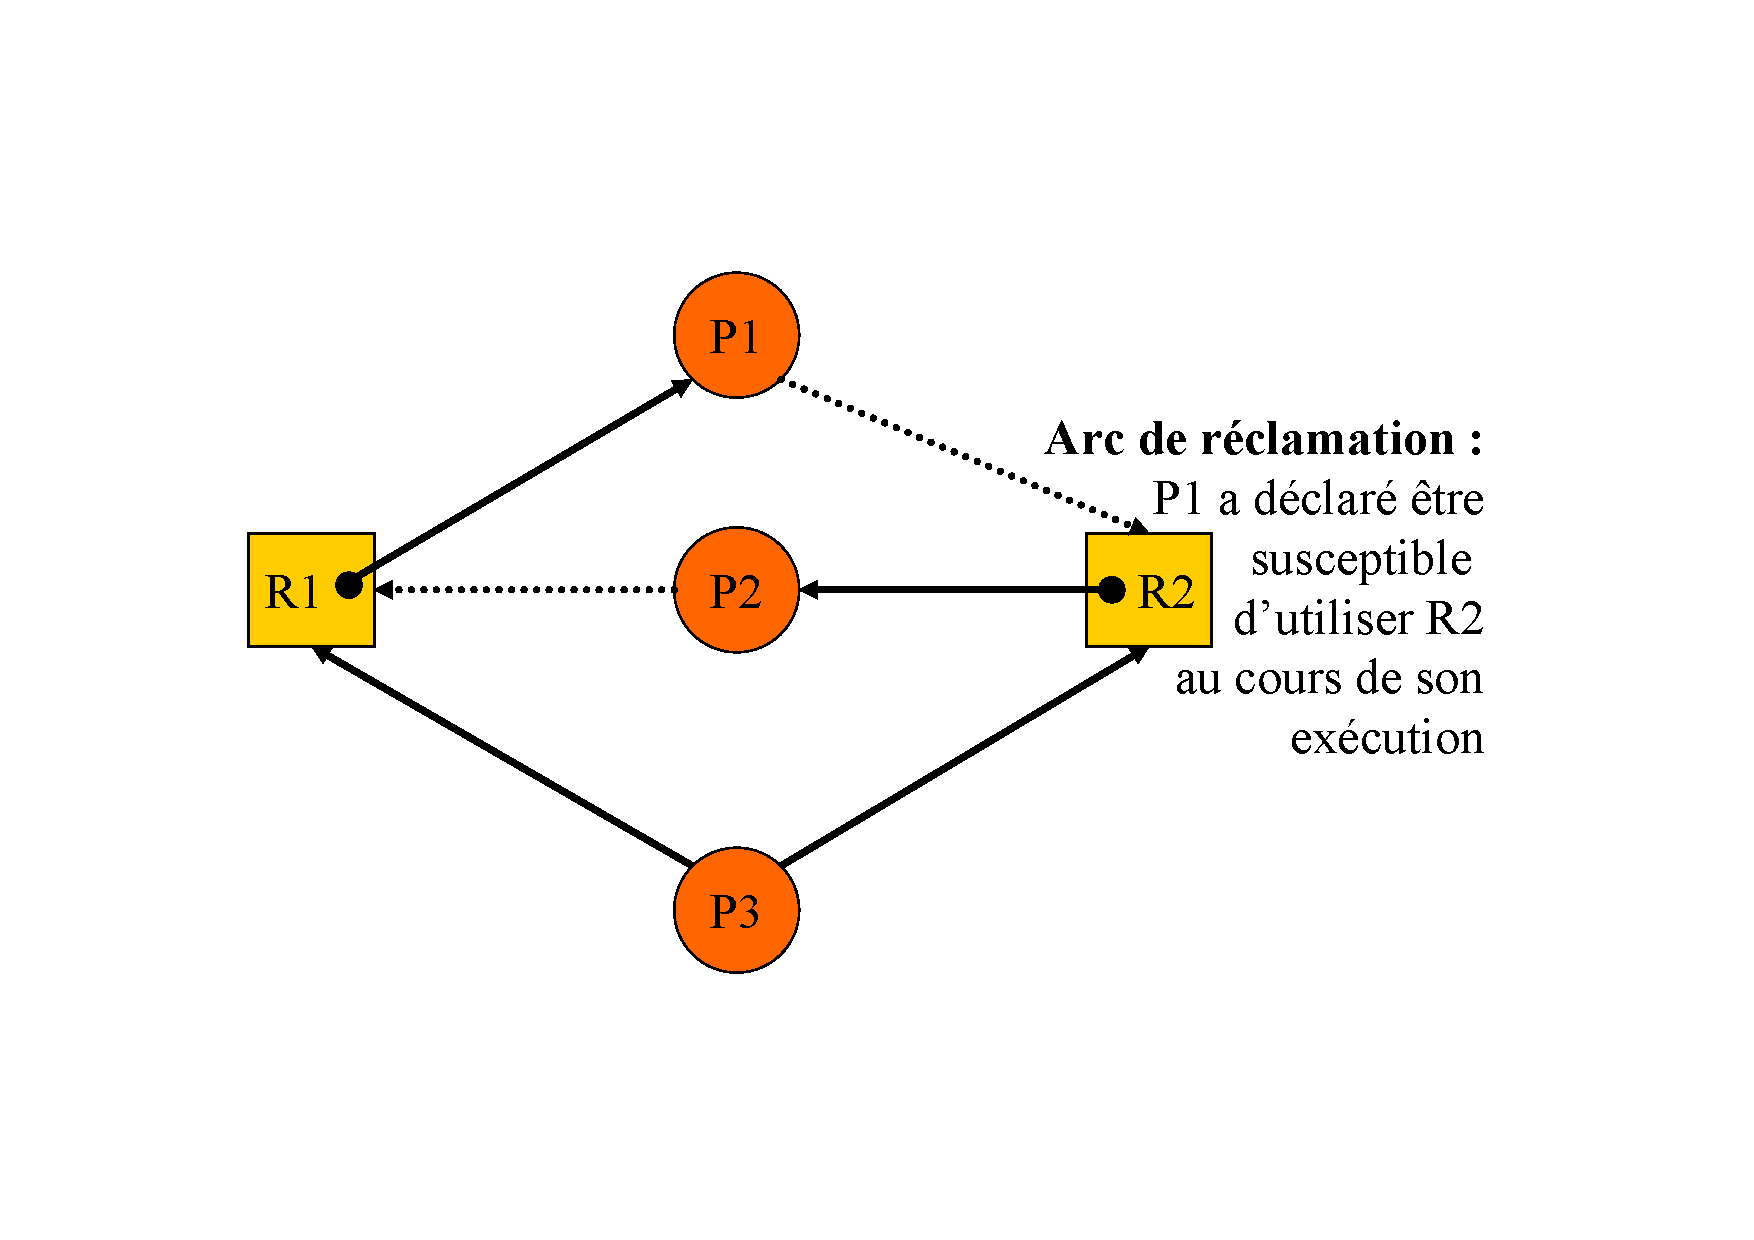
\includegraphics[width=.9\textwidth]{../illustration/arc_reclamation.pdf}
\end{frame}

\begin{frame}
\frametitle{Éviter l’attente circulaire}
\begin{itemize}
\item Au démarrage de chaque processus, ses arcs de réclamation doivent être  positionnés dans le graphe d’allocation de ressources
\item Possibilité d’ajouter un arc de réclamation sur une ressource si cette dernière ne reçoit que des arcs de réclamation
\end{itemize}
\end{frame}

\begin{frame}
\frametitle{Éviter l’attente circulaire}
\begin{itemize}
\item Demande de ressource :
\begin{itemize}
\item Arc de réclamation $\to$ arc de requête
\end{itemize}
\item Libération de ressource :
\begin{itemize}
\item Arc d’affectation $\to$ arc de réclamation
\end{itemize}
\item <2>État sain :
\begin{itemize}
\item Pas de cycle dans le graphe d’allocation
\item Algorithme de détection de cycle lancé à chaque changement du graphe
\end{itemize}
\end{itemize}
\end{frame}

\begin{frame}
\frametitle{Éviter l’attente circulaire}
\begin{columns}
\column{0.45\textwidth}
État sain et fiable :
\begin{itemize}
\item Pas de cycle
\end{itemize}
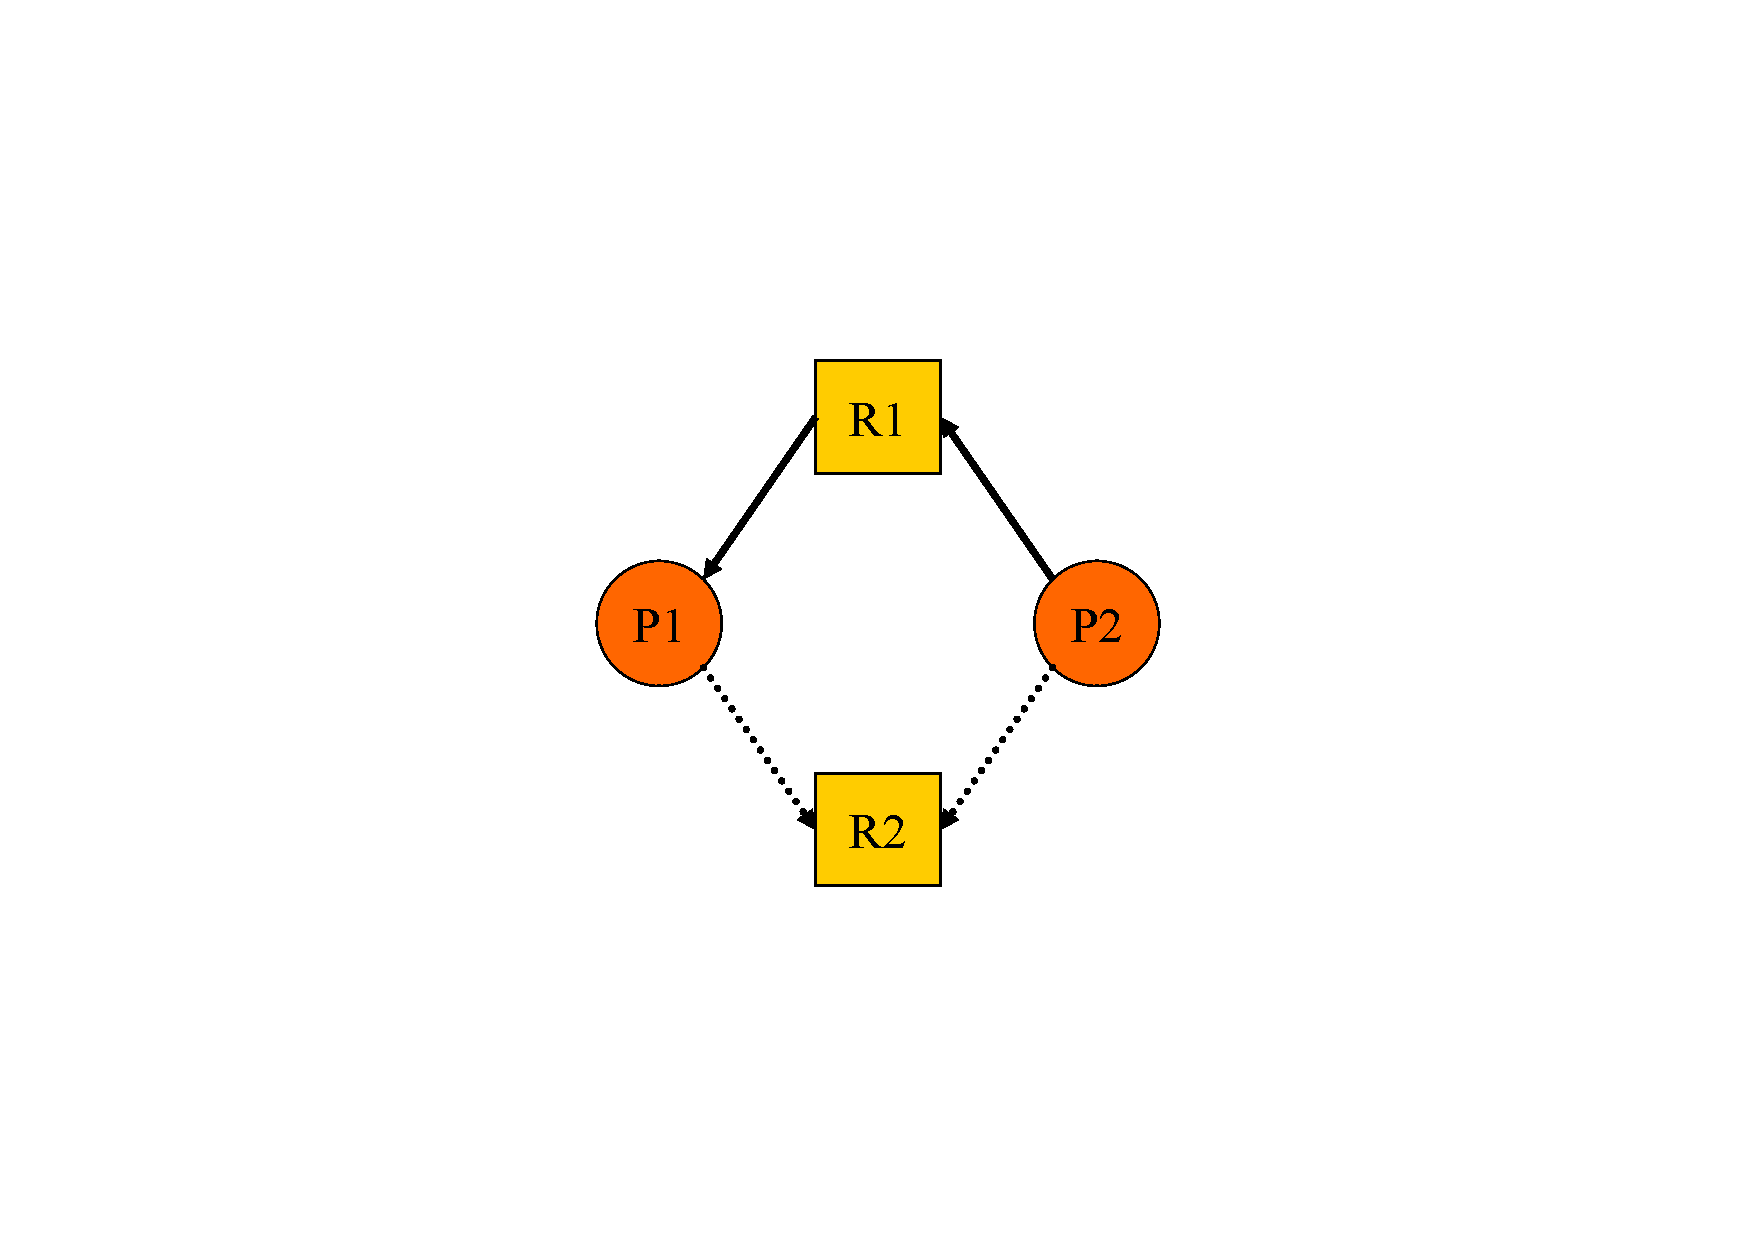
\includegraphics[width=5cm]{../illustration/ga_pas_cycle.pdf}
\column{0.45\textwidth}
État sain, mais pas fiable :
\begin{itemize}
\item Refus de la requête
\end{itemize}
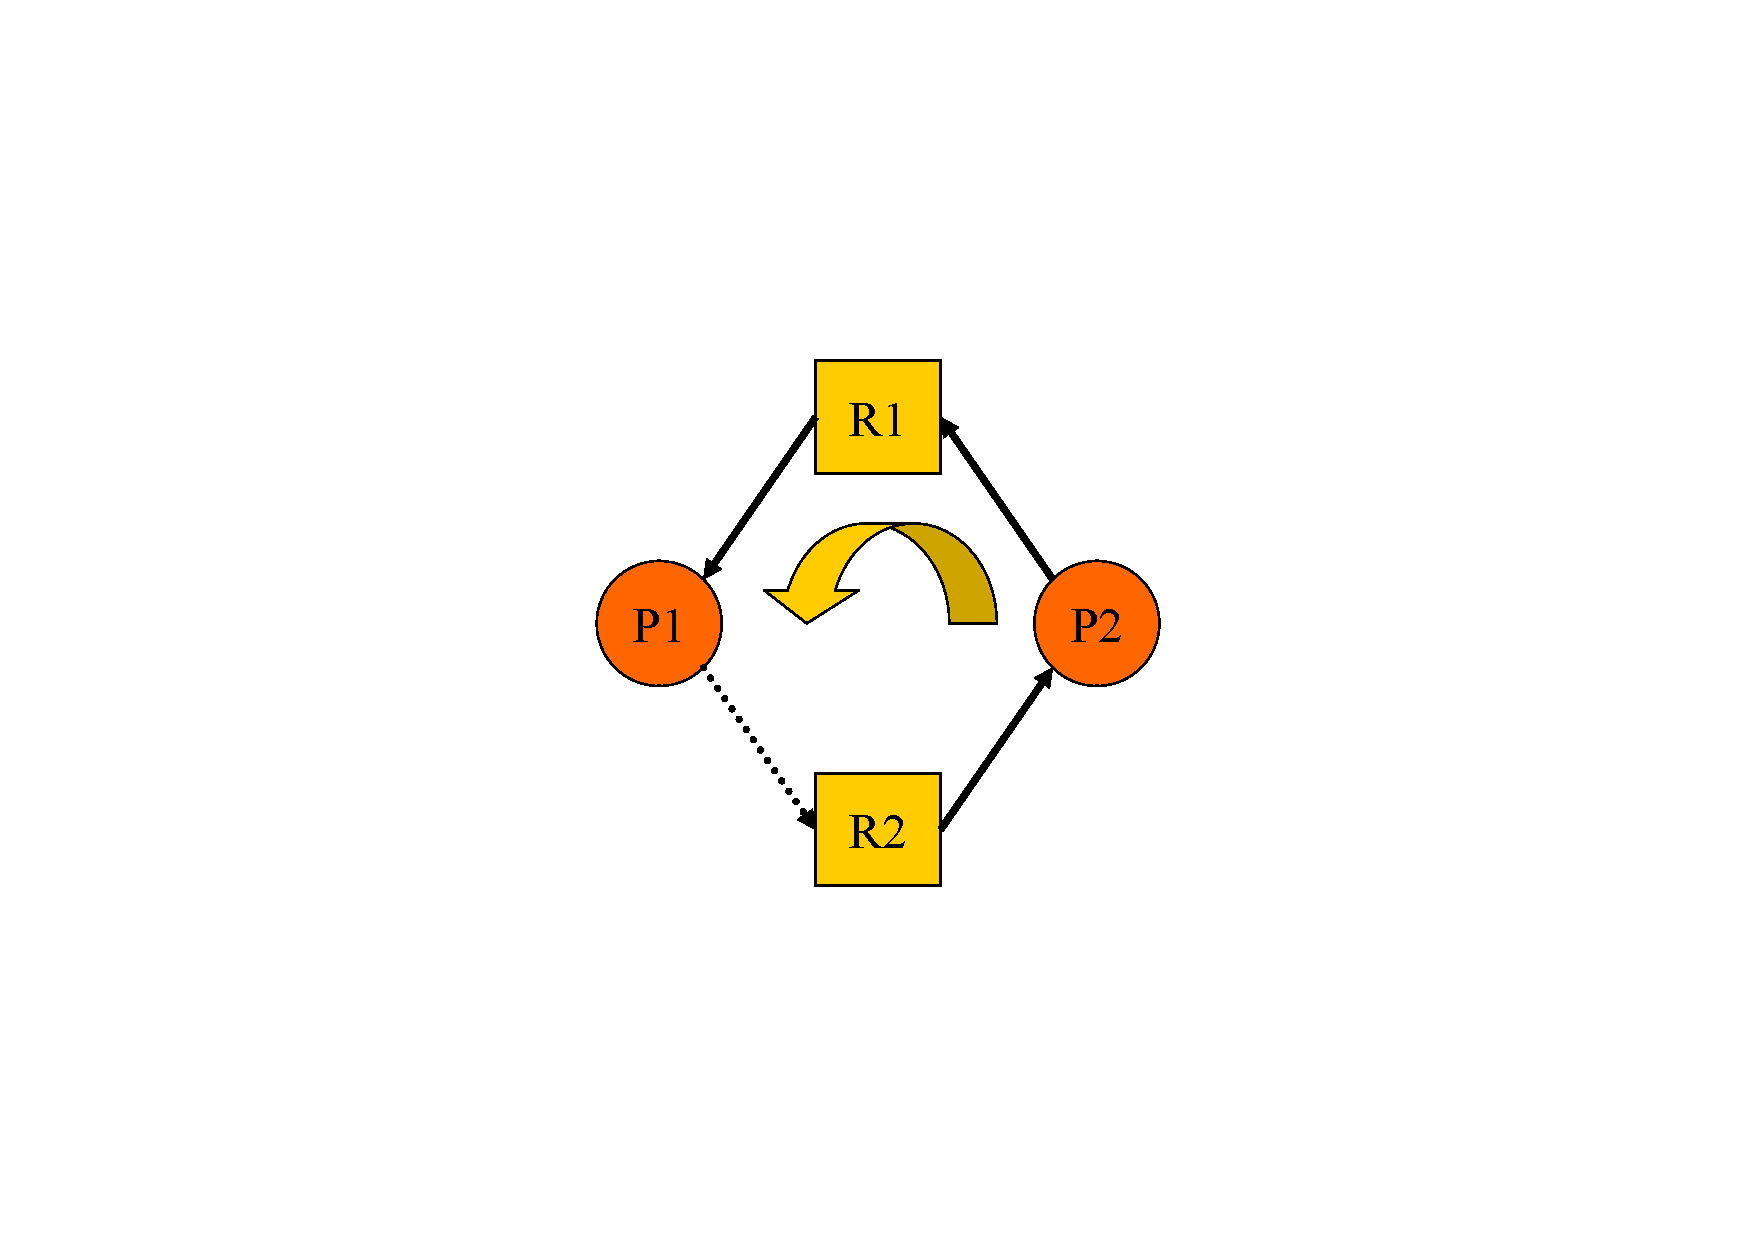
\includegraphics[width=5cm]{../illustration/ga_cycle.pdf}
\end{columns}
\end{frame}

\begin{frame}
\frametitle{Algorithme du banquier}
\begin{itemize}
\item Mis au point par Edsger Dijkstra en 1965
\item Reproduit le modèle du prêt à des clients par un banquier
\begin{itemize}
\item Nombre maximal de ressources
\begin{itemize}
\item Crédit total du processus
\end{itemize}
\item Nombre alloué
\begin{itemize}
\item Encours du processus
\end{itemize}
\item Etat fiable s'il existe une suite d'états ultérieurs qui permette à tous les processus d'obtenir toutes les ressources demandées et de se terminer
\end{itemize}
\end{itemize}
\end{frame}

\begin{frame}
\frametitle{Algorithme du banquier}
\framesubtitle{Exemple}
\begin{tabular}{|c|c|c|c|c|c|c|c|c|}
\hline
Processus & \multicolumn{4}{c|}{Ressources attribuées} & \multicolumn{4}{c|}{Ressources demandées} \\
 & R1 & R2 & R3 & R4 & R1 & R2 & R3 & R4 \\
\hline
P1   &3&0&1&1&1&1&0&0 \\
P2   &0&1&0&0&0&1&1&2\\
P3   &1&1&1&0&3&1&0&0\\
P4   &1&1&0&1&0&0&1&0\\
P5   &0&0&0&0&2&1&1&0\\
\hline
Total&5&3&2&2&6&4&3&2\\
\hline
\end{tabular}

\begin{center}
\begin{tabular}{|l|c|c|c|c|}
\hline
& R1 & R2 & R3 & R4 \\
\hline
Quantité dispo & 6 & 4 & 3 & 2 \\
Quantité restante & 1 & 1 & 1 & 0 \\
\hline
\end{tabular}
\end{center}
\end{frame}

\begin{frame}
\frametitle{Algorithme du banquier}
\framesubtitle{Exemple}
L'algorithme suivant détermine si un état est sûr :
\begin{itemize}
\item <1->Trouver dans le tableau de droite une ligne L dont les ressources demandées sont toutes inférieures aux dispo
\begin{itemize}
\item Si L n'existe pas $\rightarrow$ l'état n'est plus sain $\rightarrow$ interblocage.
\end{itemize}

\item <2->Supposer que le processus associé à L obtient les ressources et se termine
\begin{itemize}
\item Supprimer sa ligne et actualiser les disponibilités
\end{itemize}

\item <3->Répéter 1 et 2 jusqu'à ce que tous les processus soient terminés
\end{itemize}
\end{frame}

\begin{frame}
\frametitle{Algorithme du banquier}
\framesubtitle{Exemple}
Dans cet exemple, l'état actuel est fiable car :
\begin{itemize}
\item on allouera à P4 les ressources demandées et il s'achèvera
\item puis on allouera à P1 ou P5 les ressources demandées et P1 ou P5 s'achèvera
\item enfin les autres
\end{itemize}
\end{frame}

\begin{frame}
\frametitle{Algorithme du banquier}
\framesubtitle{Structures de données nécessaires}
\begin{itemize}
\item Utilisation des variables suivantes :
\begin{itemize}
\item [Free (R)] Nombre de ressources disponibles de chaque type
\item [Max (P, R)] Réclamation maximale de chaque ressource par processus
\item [Used (P, R)] Nombre de ressources occupées par processus
\item [Need (P, R)] Max - Used
\end{itemize}
\end{itemize}
\end{frame}

\begin{frame}
\frametitle{Algorithme du banquier}
\framesubtitle{Effets secondaires}
\begin{itemize}
\item Moindre utilisation des ressources
\item Réduction de la capacité de traitement du système
\item Possibilité d’une famine de ressources
\end{itemize}

Caractère irréaliste de la connaissance préalable des ressources nécessaires à l'achèvement d'un processus.

Dans bien des systèmes, ce besoin évolue dynamiquement.
\end{frame}

\begin{frame}
\frametitle{Ignorer le problème : Principe}
\begin{itemize}
\item Considérer qu’il n’y a jamais d’interblocage dans le système :
\begin{itemize}
\item Coûts de prévention et de lutte plus coûteux que le blocage occasionnel du système
\item Responsabiliser des programmeurs
\end{itemize}
\item L’interblocage n’est pas la seule source de blocage du système
\begin{itemize}
\item Utilisation des mêmes techniques de déblocage
\end{itemize}
\end{itemize}
\end{frame}

\begin{frame}
\frametitle{Ignorer le problème : Principe}
\begin{itemize}
\item Il n’existe pas encore de solution globale complètement satisfaisante
\item La plupart des systèmes ne cherche pas à traiter ce phénomène
\item Ne résout pas le problème dans sa généralité :
\begin{itemize}
\item Cherche uniquement à minimiser les risques
\end{itemize}
\end{itemize}
\begin{exampleblock}{Exemples de systèmes d'exploitation non fiables}
Unix, Windows NT
\end{exampleblock}

\end{frame}

\begin{frame}
\frametitle{Ignorer le problème}
\framesubtitle{Exemple de Java}
\begin{itemize}
\item Pas de mécanisme de protection des interblocages dans la JVM
\item Responsabilité du programmeur
\item Suppression des instructions pouvant engendrer des situations d’interblocage :
\begin{itemize}
\item \texttt{suspend}(), \texttt{resume}()
\end{itemize}
\end{itemize}
\includegraphics[width=2cm]{../illustration/java.png}
\end{frame}



\section{Outils avancés de synchronisation}

\subsection{Limites des sémaphores}
\begin{frame}
\frametitle{Limites des sémaphores}
\begin{itemize}
\item <1-> Outil efficace permettant de résoudre de nombreux problèmes de synchronisation
\item <1-> Simple et versatile
\item <2-> Risques lors de l’utilisation incorrecte des sémaphores :
\begin{itemize}
\item Erreurs de programmation difficiles à détecter
\item Blocages dans certains cas bien particuliers
\item Difficiles à reproduire et, donc, à diagnostiquer
\end{itemize}
\end{itemize}
\end{frame}

\begin{frame}
\frametitle{Exemples d’erreurs avec des sémaphores}
\begin{itemize}
\item <1-> Inversion des opérations \texttt{P()} et \texttt{V()} :\\
\begin{scriptsize}
\verbatiminput{include/semaph_erreur1.java}
\end{scriptsize}
\item <2-> Erreur de fonction :\\
\begin{scriptsize}
\verbatiminput{include/semaph_erreur2.java}
\end{scriptsize}
\item <3-> Omission d’une des opérations :\\
\begin{scriptsize}
\verbatiminput{include/semaph_erreur3.java}
\end{scriptsize}
\end{itemize}
\end{frame}
\subsection{Les moniteurs}

\begin{frame}
\frametitle{Les moniteurs}
\begin{itemize}
\item <1-> Outil évolué de synchronisation
\begin{itemize}
\item Brinch \& Hansen (1972-73)
\item Hoare (1974)
\end{itemize}
\item <2-> Un moniteur :
\begin{itemize}
\item objet encapsulant des fonctions externes
\item une seule peut s’exécuter à un moment donné
\end{itemize}
\item <3-> Évite beaucoup des interblocages possibles avec les sémaphores
\begin{itemize}
\item Diminue les risques d'erreur de programmation
\item Code plus lisible
\end{itemize}
\end{itemize}
\end{frame}

\begin{frame}
\frametitle{Moniteurs}
\begin{itemize}
\item <1-> Exécution de chaque procédure externe du moniteur en exclusion mutuelle
\begin{itemize}
\item Un seul Thread externe peut activer le moniteur
\item En utilisant une de ses méthodes externes
\end{itemize}
\item <2-> Pas besoin de coder l’exclusion mutuelle
\begin{itemize}
\item Elle est prise en charge par le moniteur
\item Le code est donc plus lisible
\end{itemize}
\item <3-> Un thread externe ne devrait pas pouvoir se bloquer dans une méthode externe
\begin{itemize}
\item Conserve le verrou
\item Risque d'interblocage
\end{itemize}
\end{itemize}
\end{frame}

\begin{frame}
\frametitle{Exemple de moniteur}
\verbatiminput{include/exemple_moniteur.java}
\begin{itemize}
\item Seul \textbf{un exemplaire} de écrivain ou de lecteur pourra s'exécuter à un moment donné
\item Quel que soit le nombre de processus qui s'exécutent et qui font appel au moniteur
\end{itemize}
\end{frame}

\begin{frame}
\frametitle{Modèle de Hoare}
\begin{itemize}
\item <1-> Amélioration du modèle initial
\item <2-> Ajout d'un mécanisme permettant à un processus :
\begin{itemize}
\item de s'arrêter sur une condition particulière
\item de laisser sa place
\item de reprendre son exécution quand la condition est remplie
\end{itemize}
\item <3-> Variable de type ''condition''
\end{itemize}
\end{frame}

\begin{frame}
\frametitle{Composants des moniteurs}
\begin{itemize}
\item <1-> Variables d'état
\begin{itemize}
\item Variables classiques, sans aucun support spécifique de synchronisation
\end{itemize}
\item <1-> Procédures internes
\begin{itemize}
\item Fonctions classiques, non synchronisées
\end{itemize}
\item <2-> Procédures externes
\begin{itemize}
\item Point d'entrée des threads externes
\item Exécution en exclusion mutuelle
\end{itemize}
\item <3-> Conditions et primitives de synchronisation\begin{itemize}
\item Permet de mettre des threads en attente en ré-affectant le verrou du moniteur à un autre thread en attente
\end{itemize}
\end{itemize}
\end{frame}

\begin{frame}
\frametitle{Les instructions spéciales des moniteurs}
\framesubtitle{Variables de type ''condition''}
\begin{itemize}
\item [Attendre] \texttt{wait(variable)} : Le thread invoquant cette opération reste bloqué sur la variable jusqu’à nouvel ordre
\item [Signaler] \texttt{signal(variable)} : Débloque un thread bloqué sur la condition. Sans effet s’il n ’existe pas de thread dans cet état
\item [Vide] \texttt{empty(variable)}: Vrai si aucun processus n'est en attente de la condition, faux sinon
\end{itemize}
\end{frame}

\begin{frame}
\begin{multicols}{2}
\begin{scriptsize}\verbatiminput{include/philo_moniteur.java}\end{scriptsize}
\end{multicols}
\begin{center}
Évite l’interblocage, pas la famine
\end{center}
\end{frame}

\subsection{Outils de synchronisation Java}

\begin{frame}
\frametitle{Outils de synchronisation Java}
\framesubtitle{Principe général du langage}
\begin{itemize}
\item <1-> Utilisation des sémaphores non encouragée
\begin{itemize}
\item Pas proposées initialement
\item Apparues dans la version 1.5
\end{itemize}
\item <2-> Méthodes ou variables \texttt{synchronized} :
\begin{itemize}
\item Empêche l’exécution simultanée par plusieurs threads d’une entité protégée d’un objet
\end{itemize}
\item <3-> Un verrou par objet (et non par entité)
\begin{itemize}
\item Gestion de file d’attente sur chaque objet verrouillé
\end{itemize}
\end{itemize}
\begin{flushright}
\includegraphics[width=1.2cm]{../illustration/java.png}
\end{flushright}
\end{frame}

\begin{frame}
\frametitle{Méthodes ou variables \texttt{synchronized}}
\framesubtitle{Utilisation des verrous}
\begin{itemize}
\item Protection d'une section critique à l'aide d'un objet verrou :
\begin{scriptsize}\verbatiminput{include/moniteur1.java}\end{scriptsize}
\item Accès exclusif au code délimité :
\begin{scriptsize}\verbatiminput{include/moniteur2.java}\end{scriptsize}
\item Accès exclusif à maFonction() :
\begin{scriptsize}\verbatiminput{include/moniteur3.java}\end{scriptsize}
\end{itemize}
\end{frame}

\begin{frame}
\frametitle{Méthodes synchronized}
\framesubtitle{Liste d'attente de verrou}
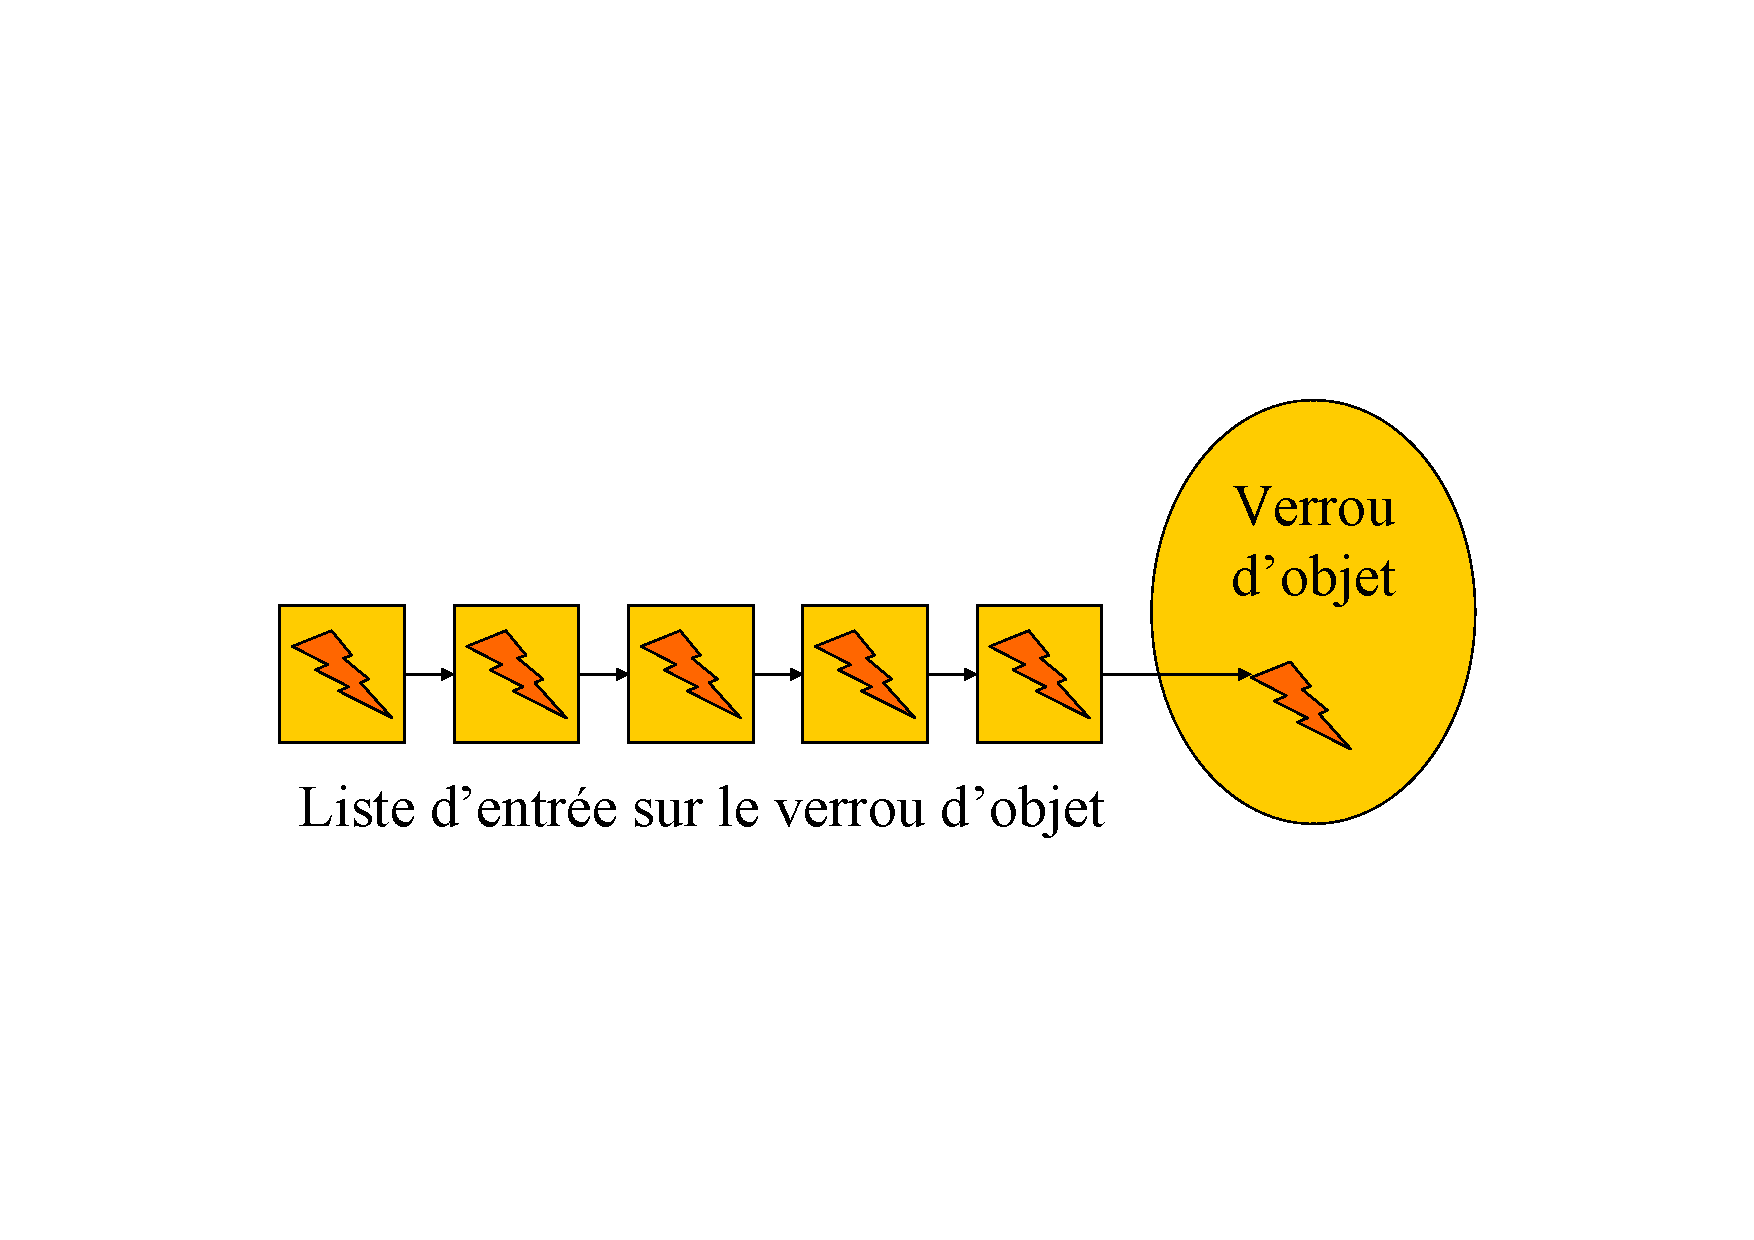
\includegraphics[width=\textwidth]{../illustration/methode_synchronized.pdf}
\end{frame}

\begin{frame}
\frametitle{Résolution du problème du tampon borné}
\begin{scriptsize}\verbatiminput{include/tb_synchro.java}\end{scriptsize}
\begin{center}
{\LARGE Mène à l'interblocage}
\end{center}
\end{frame}

\begin{frame}
\frametitle{Outils de synchronisation Java}
\framesubtitle{Problèmes potentiels}
\begin{itemize}
\item \texttt{thread.yield()} :
\begin{itemize}
\item Le thread reste exécutable (état "prêt")
\item autorise la JVM à choisir un autre thread de priorité égale
\end{itemize}
\item Méthodes \texttt{synchronized} et \texttt{yield()} :
\begin{itemize}
\item Garantissent l’exclusion mutuelle
\item Ne suppriment pas l’attente active
\item Verrouillage de l’ensemble de l’objet pendant l’attente active
\end{itemize}
\item Solution menant à un interblocage
\begin{itemize}
\item Détention et attente sur le verrou d'objet
\end{itemize}

\end{itemize}
\begin{flushright}
\includegraphics[width=1cm]{../illustration/java.png}
\end{flushright}
\end{frame}

\begin{frame}
\frametitle{Outils de synchronisation Java}
\framesubtitle{Contournement des risques de blocage}
\begin{itemize}
\item Ensemble d’attente pour chaque objet synchronisé
\item \texttt{wait()} :
\begin{itemize}
\item Permet de faire passer un thread propriétaire du verrou d’objet dans la liste d’attente (en libérant le verrou pour les threads en entrée)
\end{itemize}
\item \texttt{notify()} :
\begin{itemize}
\item Permet de faire sortir un thread de la liste d’attente vers la liste d’entrée
\end{itemize}
\item \texttt{notifyAll()} :
\begin{itemize}
\item Permet de faire sortie tous les threads de la file d’attente
\end{itemize}
\end{itemize}
\end{frame}

\begin{frame}
\frametitle{Fonctions \texttt{wait()} et \texttt{notify()}}
\framesubtitle{Ré-attribution du verrou par les threads bloqués}
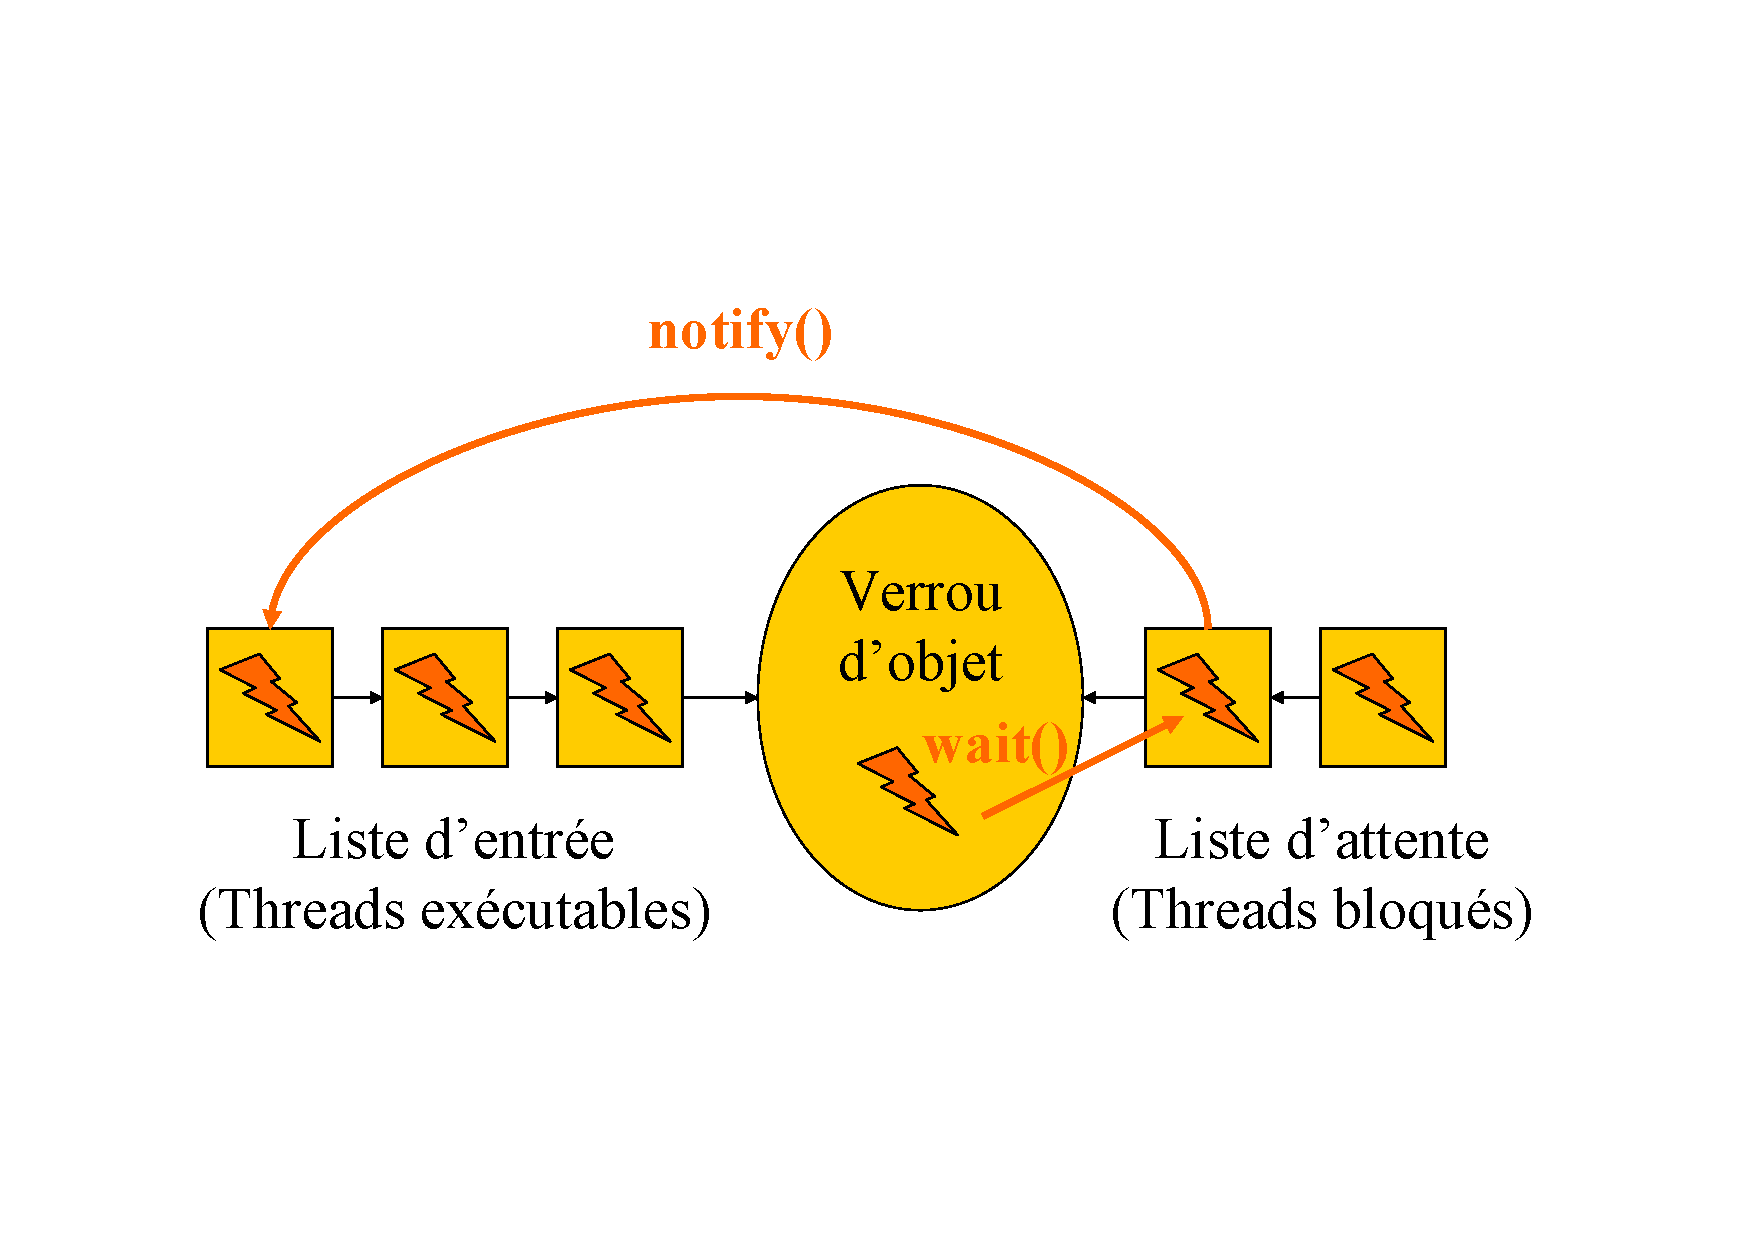
\includegraphics[width=.9\textwidth]{../illustration/methode_synchronized_notif.pdf}
\end{frame}

\begin{frame}
\frametitle{Résolution du problème du tampon borné}
\begin{scriptsize}\verbatiminput{include/tb_synchro2.java}\end{scriptsize}
\end{frame}

\begin{frame}
\frametitle{Package \texttt{java.util.concurrent.locks}}
\begin{scriptsize}
\verbatiminput{include/java_locks.java}
\end{scriptsize}
\begin{center}
Méthode plus souple que les fonctions \texttt{synchronized}
\end{center}
\end{frame}

\begin{frame}
\frametitle{Outils de synchronisation Java}
\framesubtitle{Mise en œuvre de sémaphores}
Sémaphores apparues dans Java 1.5
\begin{itemize}
\item Initialisée à une variable entière (toujours positive ou nulle)
\item P $\rightarrow$ \texttt{acquire()}
\item V $\rightarrow$ \texttt{release()}
\end{itemize}
\begin{exampleblock}{Exemple d'utilisation}
\begin{scriptsize}
 \verbatiminput{include/semaphore.java}
\end{scriptsize}
\end{exampleblock}

\end{frame}

\begin{frame}
\frametitle{Outils de synchronisation Java}
\framesubtitle{Outils de synchronisation de plus haut niveau : \texttt{listes synchronisées}}
\begin{itemize}
\item Inclus dans le paquet \texttt{java.util.concurrent}
\item Listes synchronisées
\begin{itemize}
\item \texttt{BlockingQueue} : liste bloquante non bornée
\item \texttt{ArrayBlockingQueue} : liste bloquante à tampon borné
\end{itemize}
\item Utilisables pour traiter des problèmes de type "producteur-consommateur"
\begin{itemize}
\item Comparables aux \texttt{pipe} d'Unix
\end{itemize}
\end{itemize}
\end{frame}

\begin{frame}
\frametitle{Outils de synchronisation Java}
\framesubtitle{Exemple des BlockingQueue}
\verbatiminput{include/BlockingQueue.java}
\end{frame}

\begin{frame}
\frametitle{Outils de synchronisation Java}
\framesubtitle{Outils de synchronisation de plus haut niveau : \texttt{executor}}
\begin{itemize}
\item \texttt{Executor} inclus dans le paquet \texttt{java.util.concurrent}
\begin{itemize}
\item liste d'attente d'actions à effectuer
\item traitée de façon asynchrone, mais dans l'ordre d'appel
\item un seul thread à la fois
\end{itemize}
\end{itemize}
\begin{exampleblock}{Exemple d'utilisation}
\begin{scriptsize}
\verbatiminput{include/executor.java}
\end{scriptsize}
\end{exampleblock}
\end{frame}


\subsection{Synchronisation systèmes d’exploitation}

\begin{frame}
\frametitle{Synchronisation systèmes d’exploitation}
\framesubtitle{Quelques exemples représentatifs}

\begin{itemize}
\item Sun Solaris 2\\

\includegraphics[width=2cm]{../illustration/Logo_Solaris.png}
\item Windows NT\\

\includegraphics[width=2cm]{../illustration/logo_windows.png}
\end{itemize}
\end{frame}

\begin{frame}
\frametitle{Primitives généralement proposées}
\begin{itemize}
\item Événements
\item Sections critiques
\begin{itemize}
\item Accessibles par un seul thread simultané
\end{itemize}
\item Exclusion mutuelle
\item mutex
\begin{itemize}
\item Outil de synchronisation pour un thread
\end{itemize}
\item Sémaphores
\begin{itemize}
\item Mutex pour n threads
\end{itemize}
\item Opérations atomiques
\begin{itemize}
\item Proposées dans l'API du système
\end{itemize}
\end{itemize}
\end{frame}

\begin{frame}
\frametitle{}
\begin{itemize}
\item Mutex adaptatifs
\item Variables condition
\item Sémaphores
\item Verrous lecteur-rédacteur
\end{itemize}
\begin{flushright}
\includegraphics[width=2cm]{../illustration/Logo_Solaris.png}
\end{flushright}
\end{frame}

\begin{frame}
\frametitle{Synchronisation sous Sun/Solaris}
\begin{itemize}
\item <1-> Mutex adaptatif
\begin{itemize}
\item Protège l’accès à tout élément de donnée critique
\item Section de code limitée
\end{itemize}
\item <2-> Si les données sont verrouillées :
\begin{itemize}
\item <2-> Sur un système multiprocesseur :
\begin{itemize}
\item Attente active si verrouillé par un thread actif
\item Blocage dans le cas contraire, réveil lors de la levée du verrou
\end{itemize}
\item <3-> Sur un système mono-processeur :
\begin{itemize}
\item Jamais d’attente active
\end{itemize}
\end{itemize}
\end{itemize}
\end{frame}

\begin{frame}
\frametitle{Synchronisation sous Sun/Solaris}
\framesubtitle{Héritage de priorité pour les synchronisations noyau}
\begin{itemize}
\item <1-> Le problème :
\begin{itemize}
\item Thread A de haute priorité
\item En attente d’un verrou détenu par un processus B de priorité inférieure
\end{itemize}
\item <2-> La solution proposée par Solaris
\begin{itemize}
\item B hérite de la priorité de A
\item ...jusqu’à ce qu’il libère le verrou bloquant A
\item B retrouve sa priorité initiale ensuite
\end{itemize}
\end{itemize}
\end{frame}

\begin{frame}
\frametitle{Synchronisation sous Windows NT}
\framesubtitle{Les outils de synchronisation disponibles}
\begin{itemize}
\item <1-> Sections critiques
\begin{itemize}
\item Uniquement utilisables par les threads d’un même processus
\end{itemize}
\item <2-> Mutex
\begin{itemize}
\item Utilisables par plusieurs processus
\end{itemize}
\item <3-> Sémaphores
\item <4-> Objets à événement
\begin{itemize}
\item Peut notifier un thread en attente de l’arrivée d’un événement
\end{itemize}
\end{itemize}
\begin{flushright}
\includegraphics[width=1cm]{../illustration/logo_windows.png}
\end{flushright}
\end{frame}

\begin{frame}
\frametitle{Synchronisation sous Windows NT}
\framesubtitle{Manipulation des événements}
\begin{itemize}
\item L'API Windows
\item Fonctions pour créer et manipuler des événements
\begin{itemize}
\item \texttt{CreateEvent()} et \texttt{CloseHandle()} : création et la destruction d'événements
\item \texttt{SetEvent()}, \texttt{ResetEvent()} et \texttt{PulseEvent()} : modifier l'état de l'objet
\end{itemize}
\item Lorsqu'un événement est en état non signalé :
\begin{itemize}
\item l'appel à une fonction d'attente provoquera la suspension du thread appelant
\item jusqu'à ce que l'événement passe en état signalé
\end{itemize}
\end{itemize}
\end{frame}


\section{Mécanismes de coopération inter-processus}
\subsection{Introduction}

\begin{frame}
\frametitle{Introduction}
\begin{itemize}
\item Les processus sont indépendants par défaut
\begin{itemize}
\item Hypothèse par défaut pour le système
\item N’affecte pas les autres processus
\item Ne peut être affecté par eux
\item Ne partage pas de ressources avec d’autres processus
\item \textbf{Cohabitation non coopérative}
\end{itemize}
\end{itemize}
\end{frame}

\begin{frame}
\frametitle{Introduction}
\begin{itemize}
\item Interaction avec d’autres processus du système souvent utile :
\begin{itemize}
\item Partage d’information
\item Accélération du calcul
\item Modularité
\item Commodité
\end{itemize}
\end{itemize}
\end{frame}

\begin{frame}
\frametitle{Processus coopérant}
\begin{itemize}
\item Peut affecter d’autres processus
\item Peut être affecté par d’autres processus
\item Partage des ressources avec d’autres processus
\item Accès concurrent aux données partagées
\begin{itemize}
\item Risque d’incohérence
\item Risque d’interblocage
\end{itemize}
\item Nécessité de coordination
\end{itemize}
\end{frame}

\begin{frame}
\frametitle{Mécanismes de communication inter-processus}
\begin{itemize}
\item Mémoire partagée
\item Tubes, tubes nommés
\item Fichiers avec mécanisme de verrouillage
\item Signaux asynchrones (interruption logicielle)
\item Sockets
\item Files de message
\item Sémaphores
\end{itemize}
\end{frame}

\begin{frame}
\frametitle{IPC : Inter Process Communication}
\begin{itemize}
\item \textit{Inter Process Communication}
\item Nécessite l’identification fiable des objets IPC
\begin{itemize}
\item id de l’utilisateur,
\item id de l’IPC,
\item mode d’accès...
\end{itemize}
\item Valeurs initialisées lors de la création de l’IPC
\end{itemize}
\end{frame}


\subsection{Mémoire partagée}

\begin{frame}
\frametitle{Segment de mémoire partagé}
\begin{itemize}
\item Partage d’un même espace physique par plusieurs processus
\begin{itemize}
\item Mémoire partagée = espace d’adressage commun à plusieurs processus
\item Un processus peut lire et écrire dans la mémoire partagée, comme s’il s’agissait de son propre espace d’adressage
\end{itemize}
\end{itemize}
\end{frame}

\begin{frame}
\frametitle{Segment de mémoire partagé}
\begin{itemize}
\item Segment de mémoire partagé :
\begin{itemize}
\item Existence indépendante des processus
\item Créé par un processus
\item Rattaché à un processus lorsqu’il le demande
\item Droits d’accès
\end{itemize}
\item Nécessite une synchronisation des accès
\end{itemize}
\end{frame}

\begin{frame}
\frametitle{Segment de mémoire partagé}
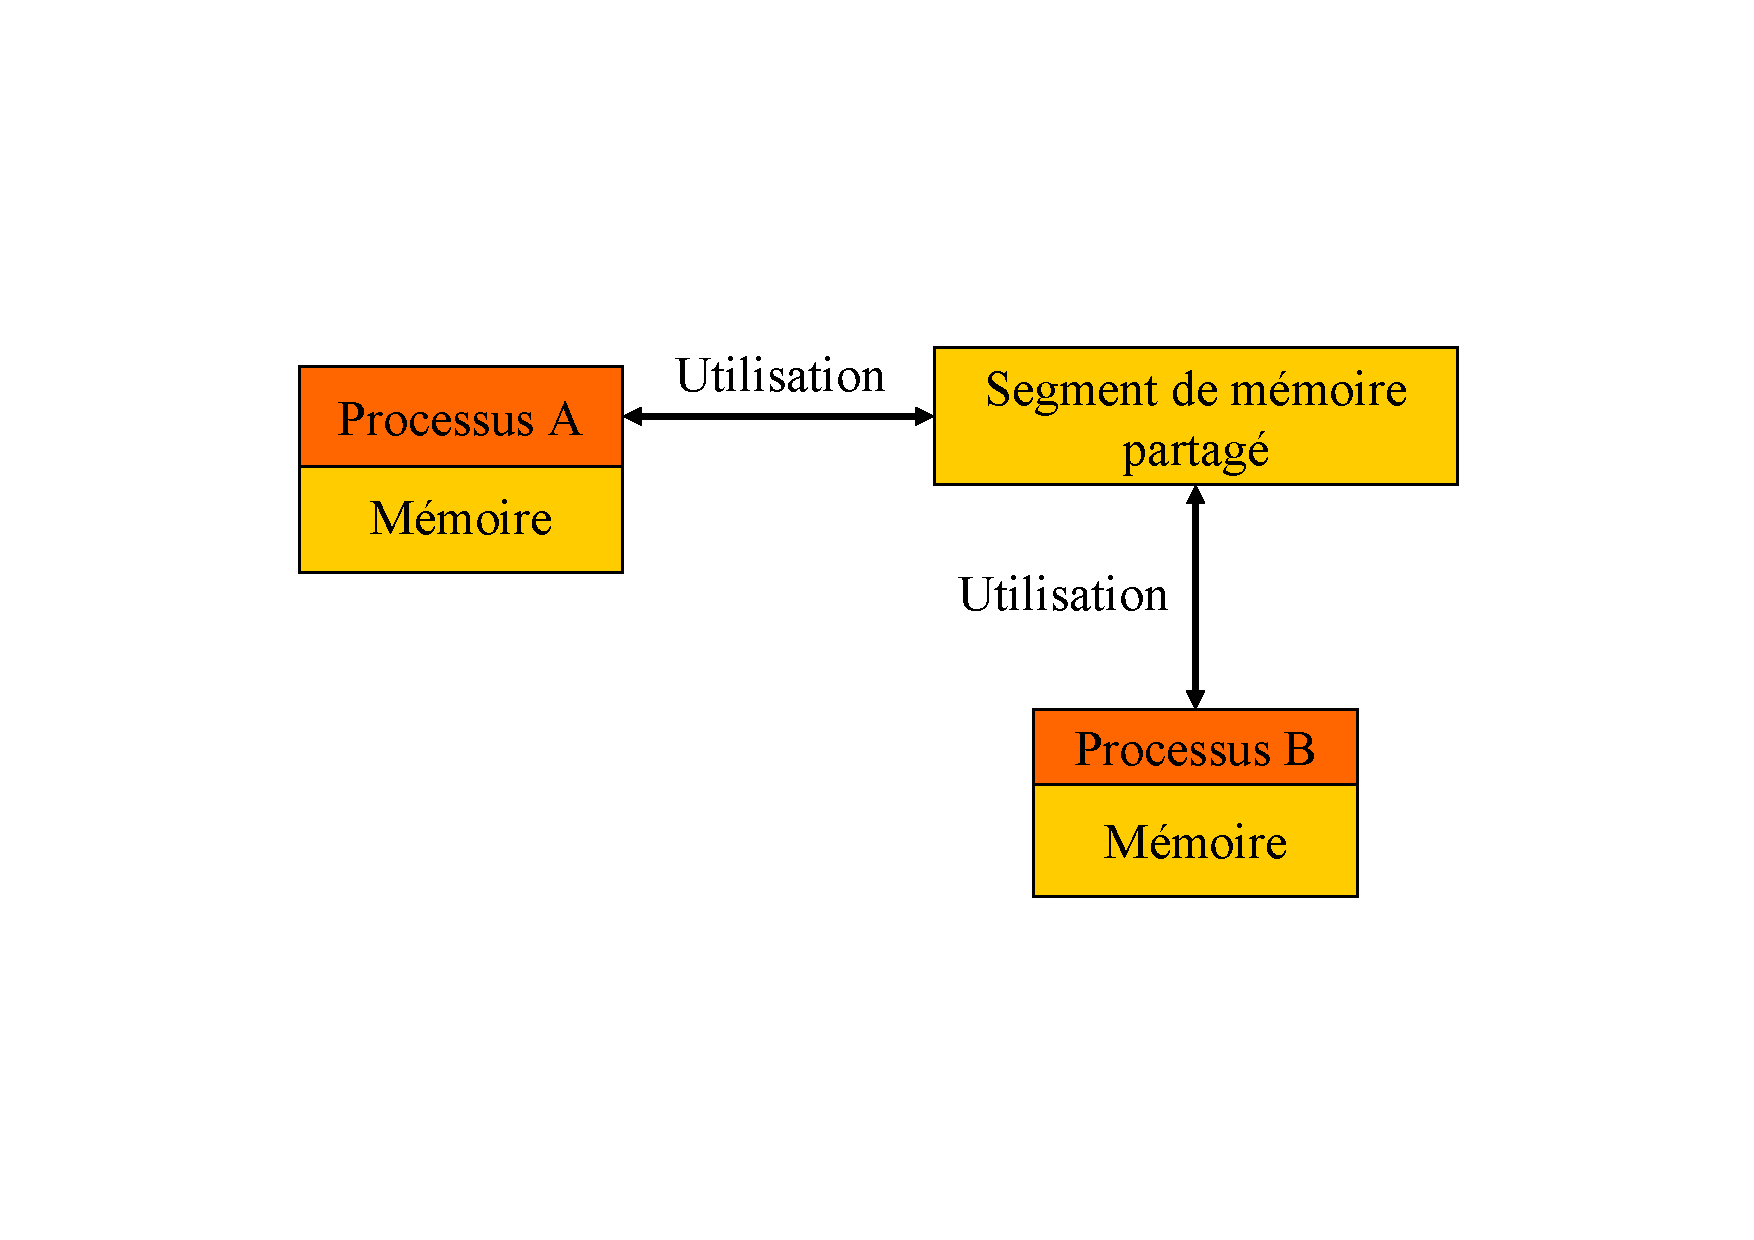
\includegraphics[width=.9\textwidth]{../illustration/segment_memoire_partagee.pdf}
\end{frame}

\begin{frame}
\frametitle{Segment de mémoire partagé (Unix System V)}
\begin{itemize}
\item Commande \texttt{shmget} :
\begin{itemize}
\item Création d’un segment de mémoire partagé
\item Utilisation d’un segment existant
\item \verbatiminput{include/shmget.c}
\end{itemize}
\item Commandes \texttt{shmat} / \texttt{shmdt} :
\begin{itemize}
\item Attachement/détachement d’un segment de mémoire partagé à l'espace d'adressage d'un processus
\end{itemize}
\item Commande \texttt{ipcs-shm} :
\begin{itemize}
\item Liste des segments de mémoire partagés
\end{itemize}
\item Commande \texttt{ipcrm} :
\begin{itemize}
\item Suppression de segment mémoire
\end{itemize}
\end{itemize}
\end{frame}

\begin{frame}
\frametitle{Segment de mémoire partagé (Windows NT)}
\begin{itemize}
\item Appelé \textit{Fichier mappé en mémoire}
\item Utilisé comme un fichier standard
\item Vitesse d’accès équivalente à celle de la mémoire
\end{itemize}
\end{frame}


\subsection{Tubes}
\begin{frame}
\frametitle{Les tubes (pipe)}
\begin{itemize}
\item Communication simple :
\begin{itemize}
\item Échange de données entre 2 processus
\item Communication à sens unique
\end{itemize}
\item Fichier spécial avec :
\begin{itemize}
\item 2 extrémités (lire/écrire)
\item Lecture destructrice
\item Gestion FIFO
\item Capacité finie
\end{itemize}
\end{itemize}
\end{frame}

\begin{frame}
\frametitle{Tubes}
\begin{itemize}
\item Autres attributs d’un tube :
\begin{itemize}
\item Nombre de lecteurs
\item Nombre d’écrivains
\end{itemize}
\item 2 types de tubes :
\begin{itemize}
\item Tubes ordinaires
\begin{itemize}
\item Communication entre processus père et fils
\item Processus de la même lignée
\end{itemize}
\item Tubes nommés
\begin{itemize}
\item Communication entre processus sans parenté
\end{itemize}
\end{itemize}
\end{itemize}
\end{frame}

\begin{frame}
\frametitle{Exemple de tube}
\begin{itemize}
\item « $\mid$ » (pipe) d’Unix :
\begin{itemize}
\item \texttt{cat fichier $\mid$ grep "toto"}
\end{itemize}
\item \texttt{grep} exploite le flux généré par \texttt{cat}
\item \texttt{grep} est le fils de \texttt{cat}
\end{itemize}
Les deux commandes s’exécutent indépendamment sauf :
\begin{itemize}
\item Si le tampon est vide : \texttt{grep} attend \texttt{cat}
\item Si le tampon est plein : \texttt{cat} attend \texttt{grep}
\end{itemize}
\end{frame}

\begin{frame}
\frametitle{Étapes d’un échange père fils avec tube}
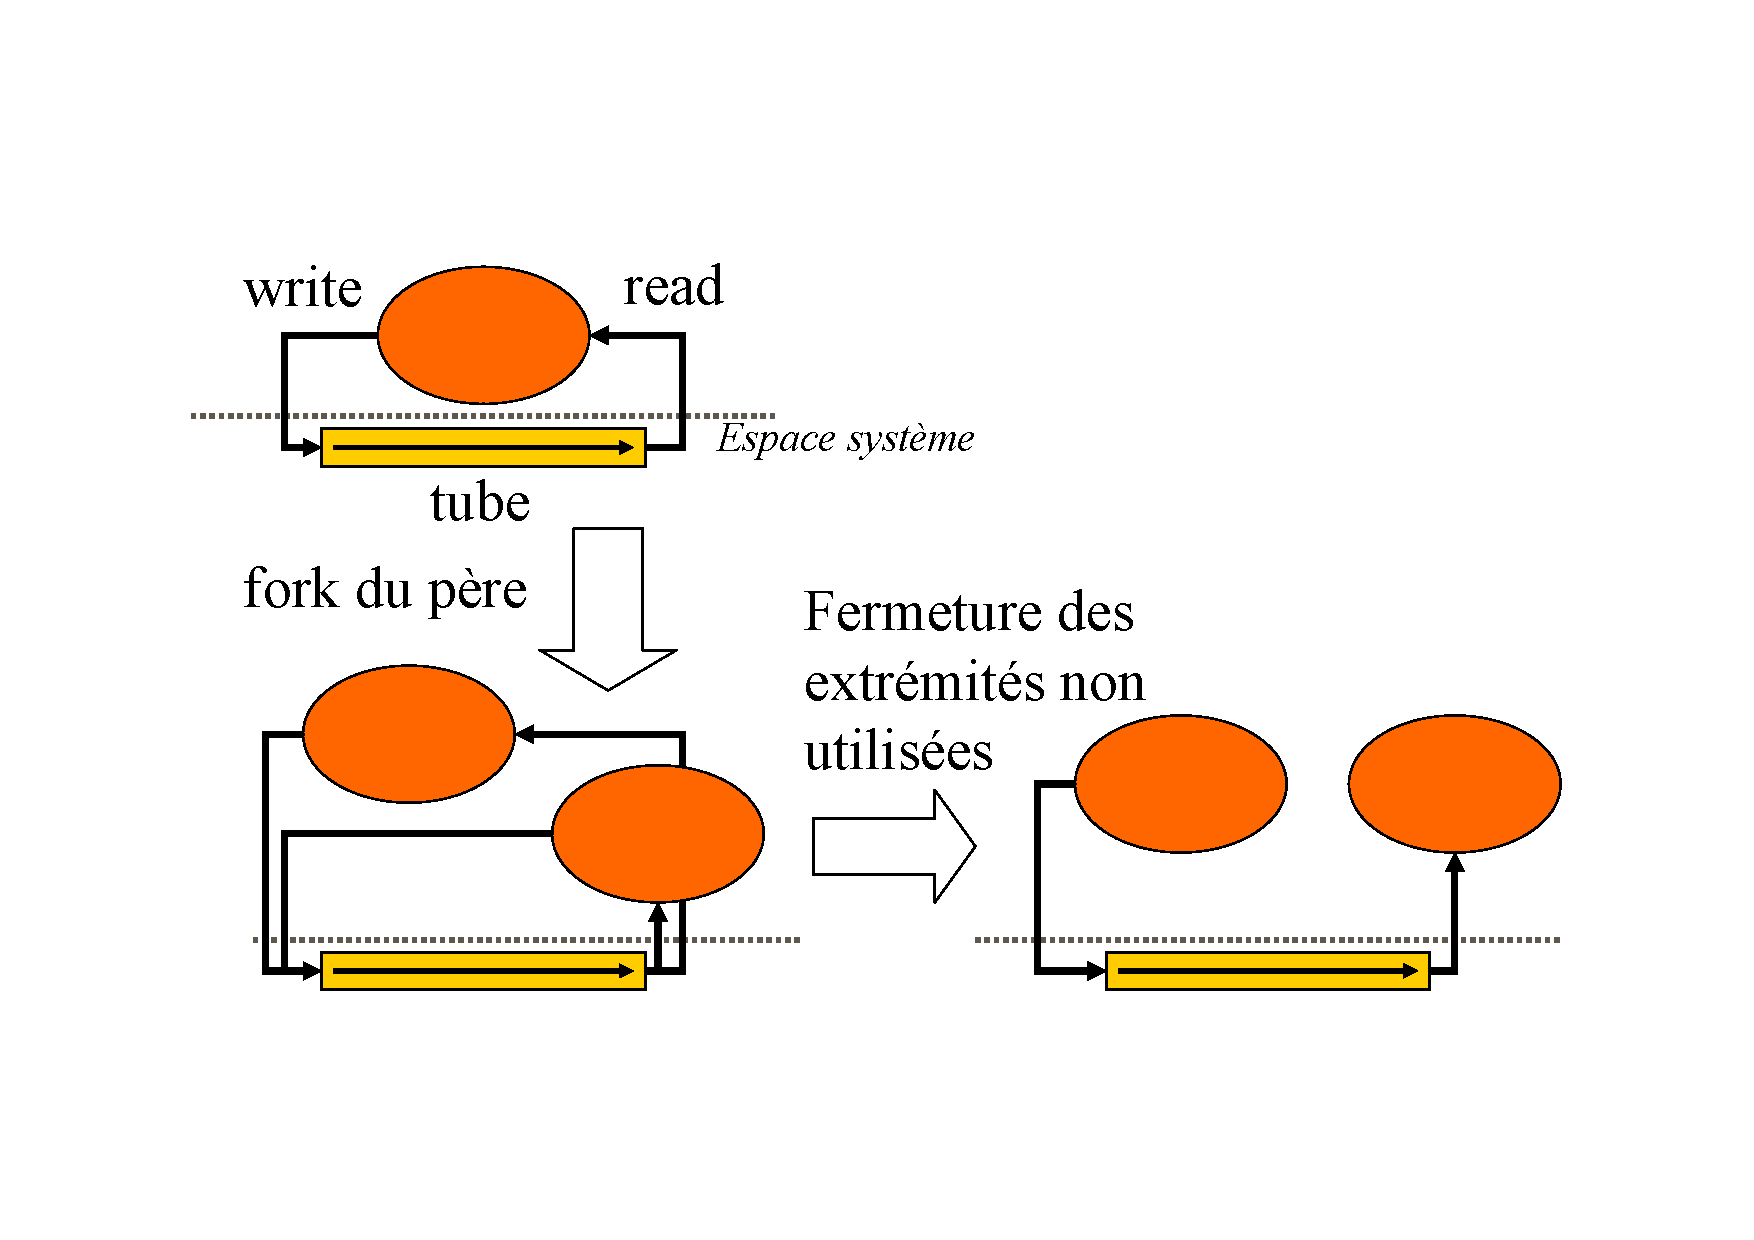
\includegraphics[width=.9\textwidth]{../illustration/tube_fork.pdf}
\end{frame}

\begin{frame}
\frametitle{Exemple en C}
\begin{scriptsize}\verbatiminput{include/tube.c}\end{scriptsize}
\end{frame}

\begin{frame}
\frametitle{Échanges client serveur avec tubes}
\begin{itemize}
\item Création de \texttt{tube1} et \texttt{tube2}
\item \texttt{fork()}
\item Le père ferme \texttt{out} de \texttt{t1} et \texttt{in} de \texttt{t2}
\item Le fils ferme \texttt{in} de \texttt{t1} et \texttt{out} de \texttt{t2}
\end{itemize}
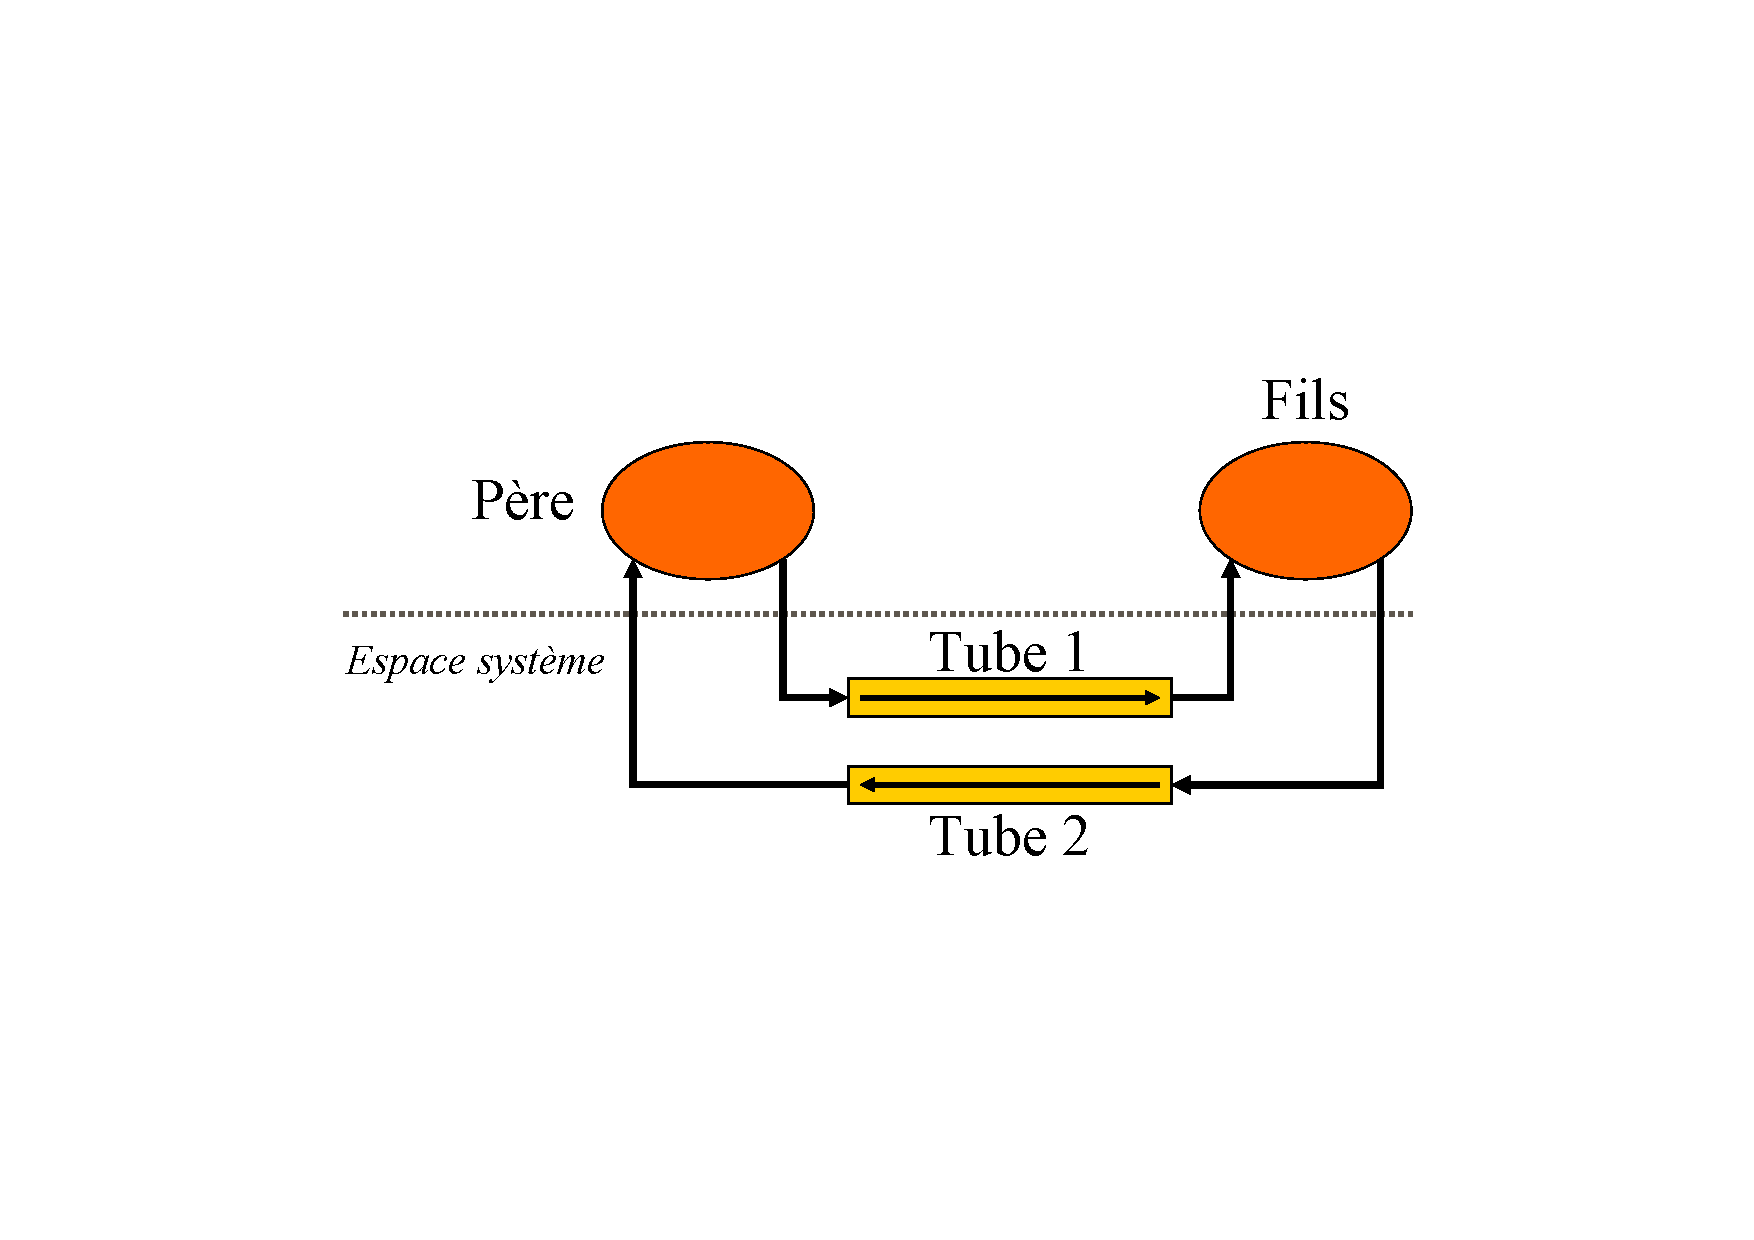
\includegraphics[width=.9\textwidth]{../illustration/tube_cs.pdf}
\end{frame}

\begin{frame}
\frametitle{Exemple de tube nommé}
\begin{itemize}
\item Tubes publics
\begin{itemize}
\item Non réservés à la seule descendance
\end{itemize}
\item Création du tube (Unix)
\begin{itemize}
\item Création d’un fichier spécial
\begin{itemize}
\item \texttt{mkfifo mon\_tube}
\end{itemize}
\item Utilisable comme un fichier normal sauf que :
\begin{itemize}
\item La taille est nulle, sauf lors de l’utilisation
\item L’écriture est bloquante
\item La lecture est destructive
\end{itemize}
\end{itemize}
\end{itemize}
\end{frame}

\begin{frame}
\frametitle{Exemple de tube nommé (Unix)}
\begin{scriptsize}\verbatiminput{include/tube.txt}\end{scriptsize}
\end{frame}

\begin{frame}
\frametitle{Client-serveur avec des tubes nommés}
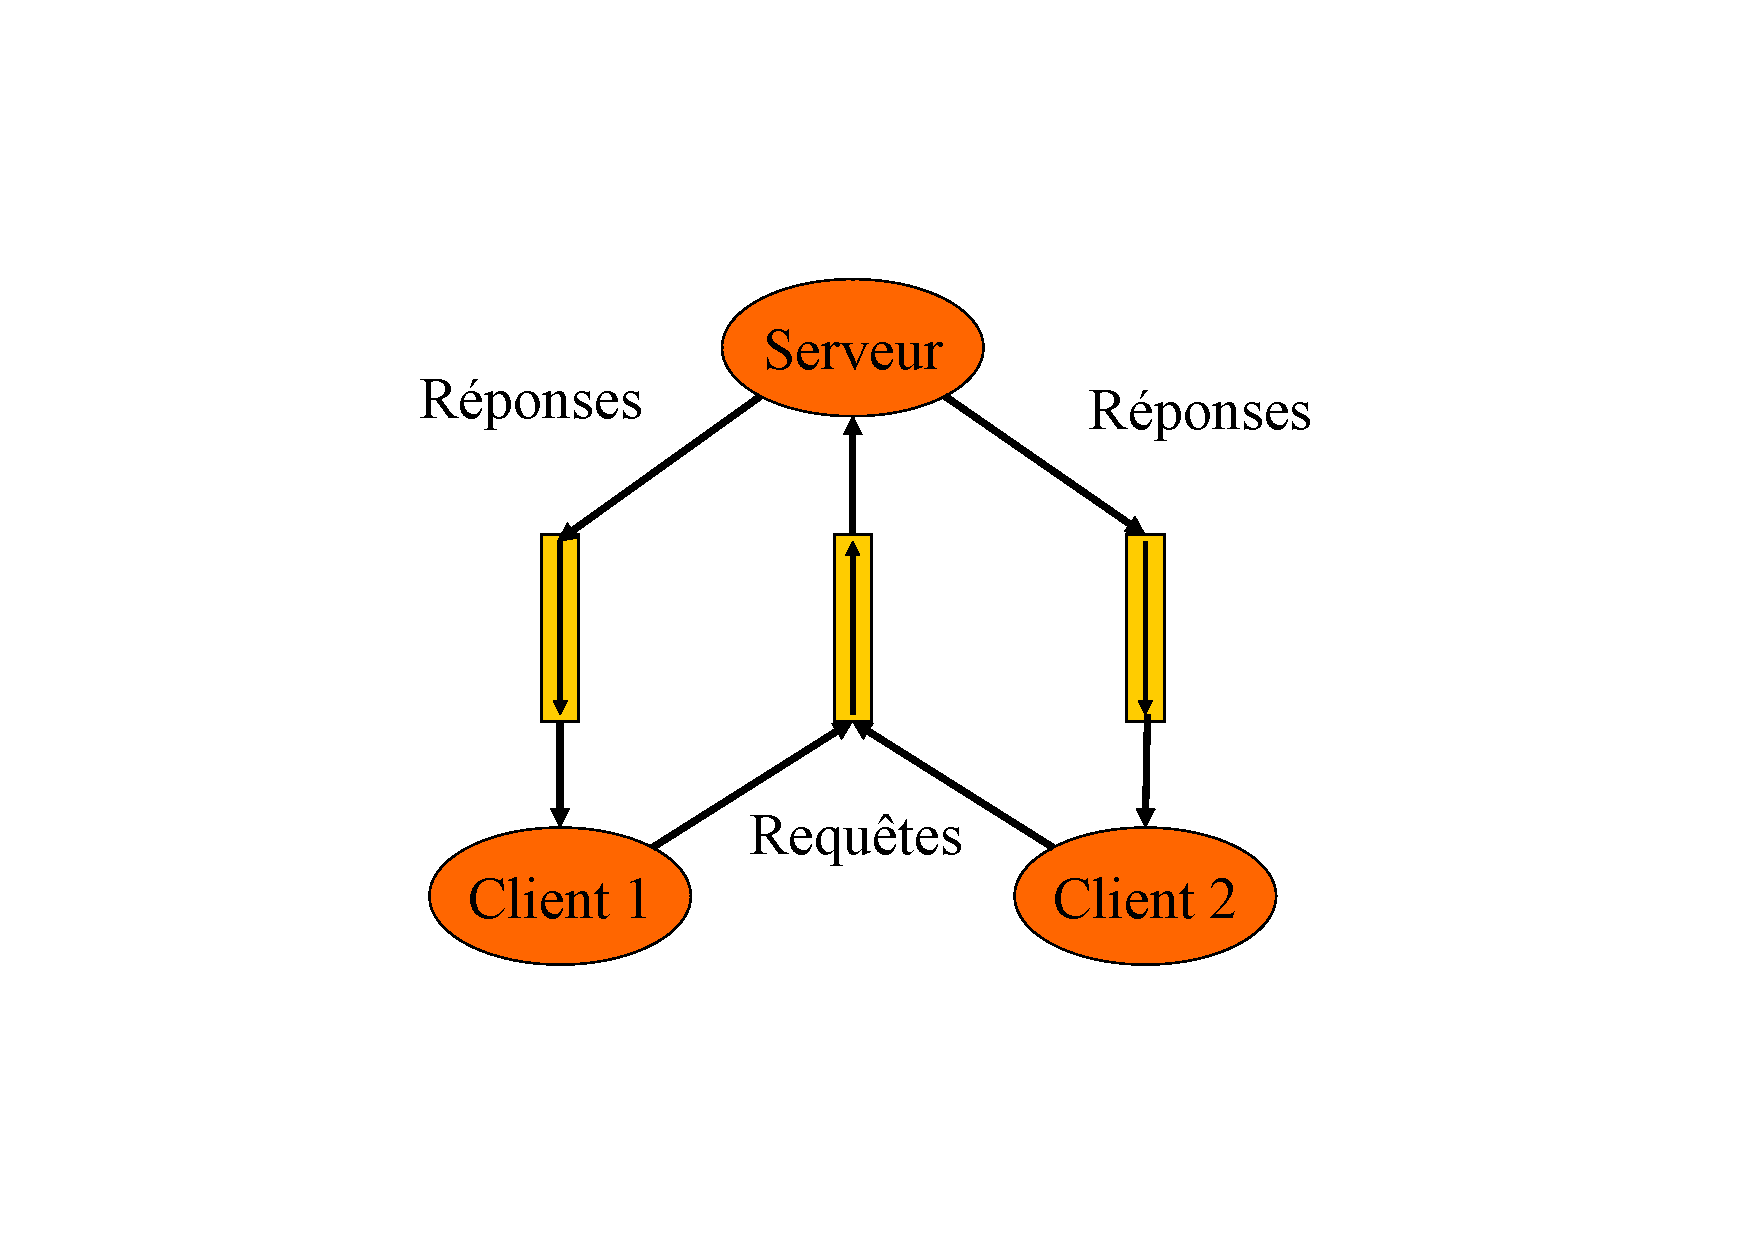
\includegraphics[height=.9\textheight]{../illustration/tube_nomme_cs.pdf}
\end{frame}

\subsection{Passage de messages}
\begin{frame}
\frametitle{Passage de messages}
\begin{itemize}
\item Au moins deux opérations :
\begin{itemize}
\item \texttt{send} (message) : envoi un message à un autre processus
\item \texttt{receive} (variable message) : reçoit un message d’un autre processus
\end{itemize}
\item Pas d’espace d’adressage communs
\end{itemize}
\end{frame}

\begin{frame}
\frametitle{Passage de messages}
\begin{itemize}
\item Communication
\begin{itemize}
\item Directe ou indirecte
\item Symétrique ou asymétrique
\item Mise en tampon
\item Copie / référence
\item Message taille fixe / variable
\end{itemize}
\item Lien de communication entre les processus
\begin{itemize}
\item Nommage des interlocuteurs
\end{itemize}
\end{itemize}
\end{frame}

\begin{frame}
\frametitle{Communication directe symétrique}
\begin{columns}
\column{0.45\textwidth}
\texttt{send}(B, Message)
\column{0.45\textwidth}
\texttt{receive}(A, message)
\end{columns}
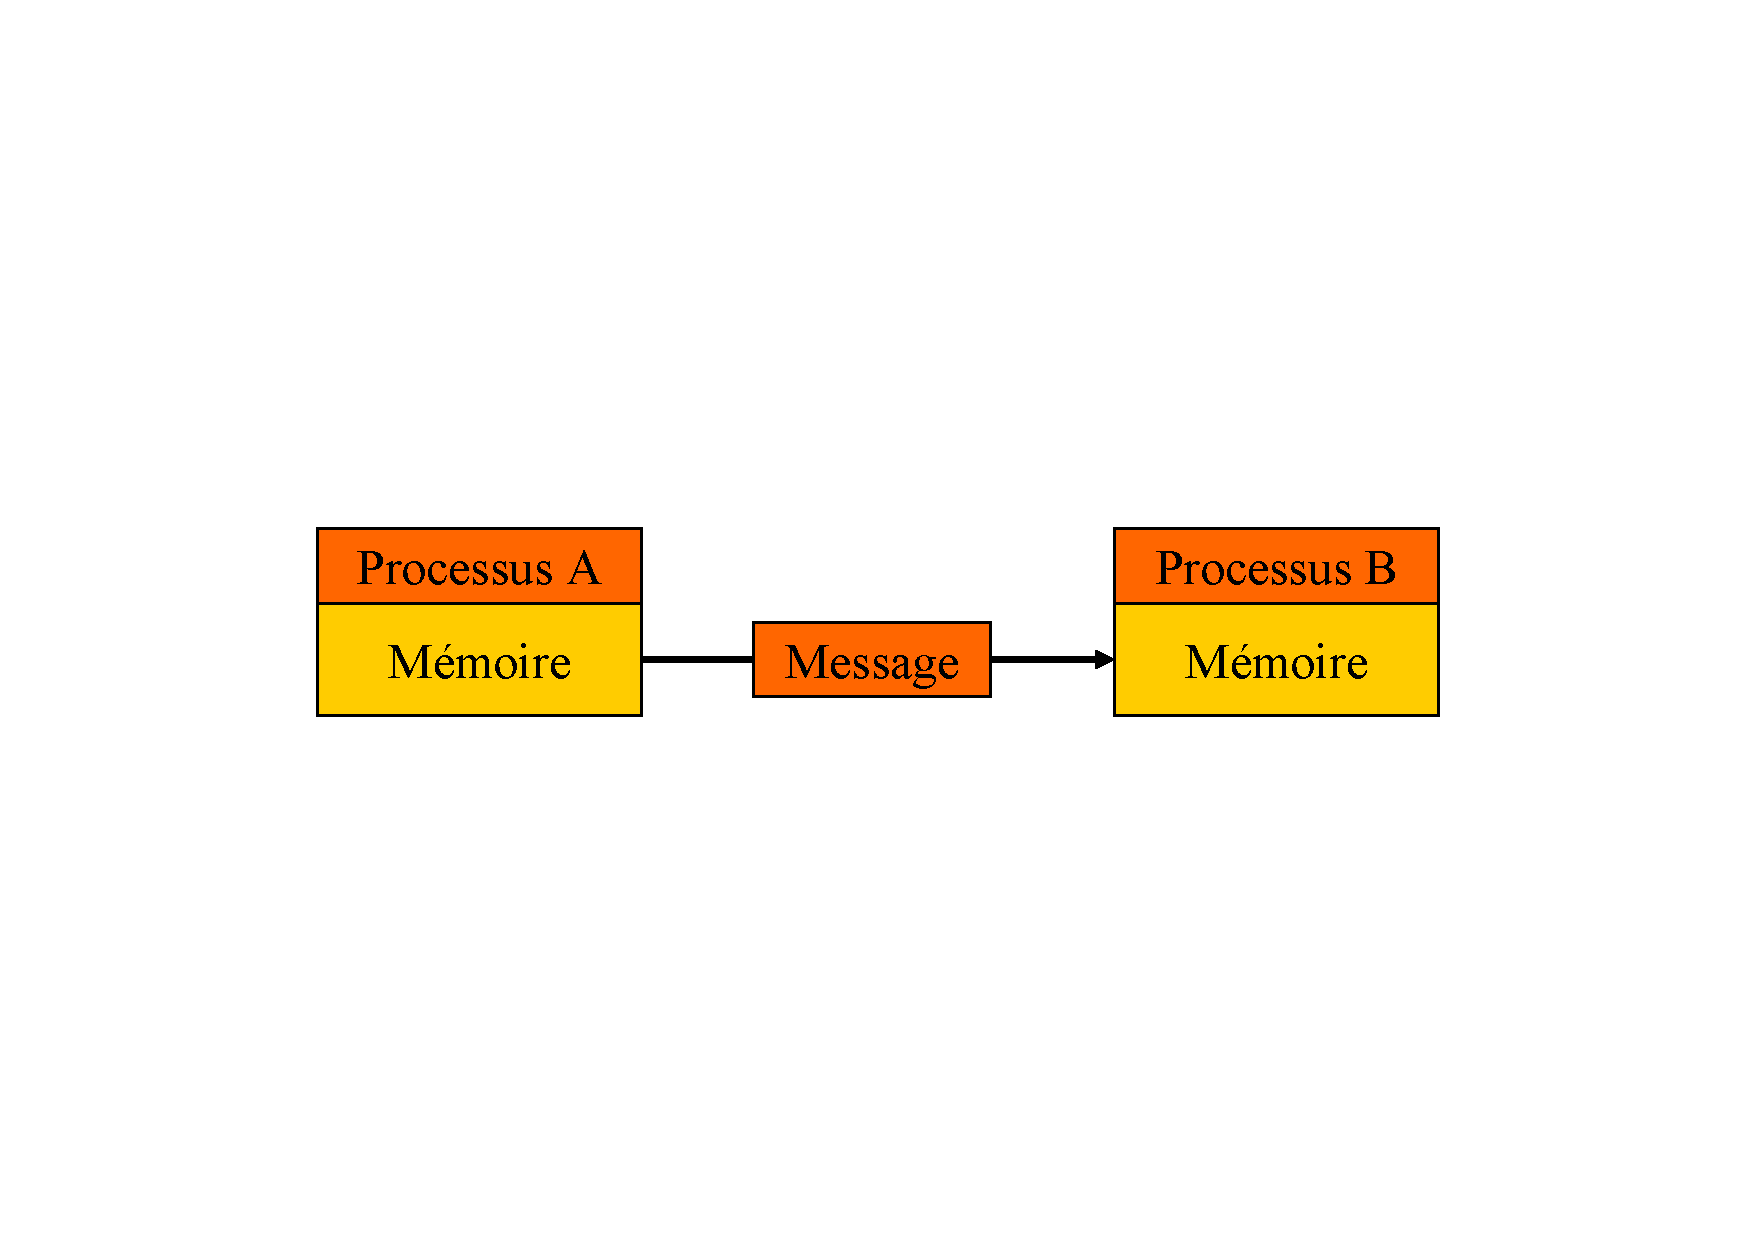
\includegraphics[width=.9\textwidth]{../illustration/message_comm_directe.pdf}
\begin{itemize}
\item A envoi un message à B
\item B attend le message de A
\end{itemize}
\end{frame}

\begin{frame}
\frametitle{Communication directe asymétrique}
\begin{columns}
\column{0.45\textwidth}
\texttt{send}(B, Message)
\column{0.45\textwidth}
\begin{itemize}
\item \texttt{receive}(id, message)
\item id = A
\end{itemize}
\end{columns}
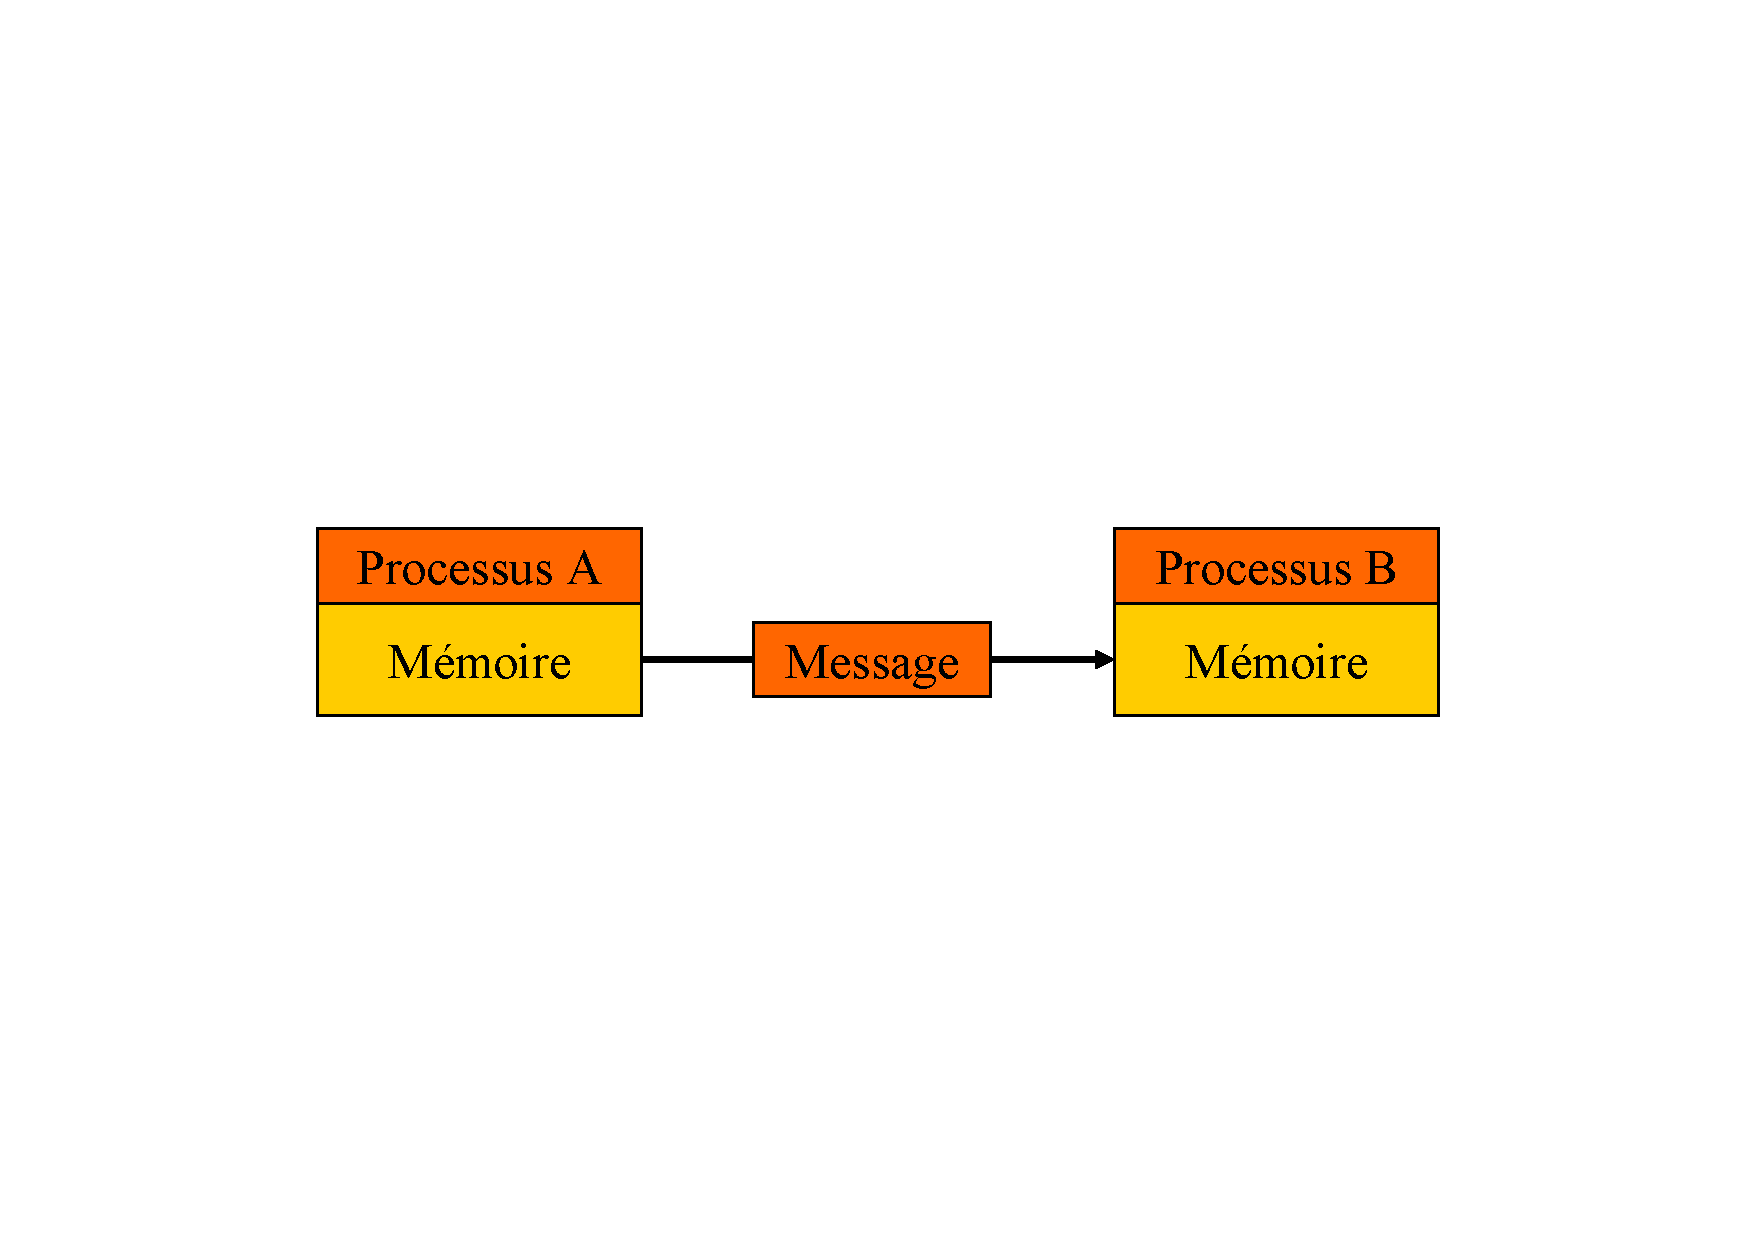
\includegraphics[width=.9\textwidth]{../illustration/message_comm_directe.pdf}
\begin{itemize}
\item A envoi un message à B
\item B attend un message
\item Identification de l’expéditeur après réception (id)
\end{itemize}
\end{frame}

\subsection{Signaux asynchrones}
\begin{frame}
\frametitle{Les signaux asynchrones}
\begin{itemize}
\item Idée :
\begin{itemize}
\item Avertir un processus d’un événement extérieur (interr. logicielle)
\end{itemize}
\item En recevant un signal, le processus peut :
\begin{itemize}
\item L’ignorer
\item Mourir / stopper
\item Se réveiller
\item Exécuter une fonction donnée
\end{itemize}
\item Liste fixée de signaux pour un OS
\end{itemize}
\end{frame}

\begin{frame}
\frametitle{Signaux asynchrones}
\begin{itemize}
\item Exemple : Commande « \texttt{kill} » de Unix
\begin{itemize}
\item \texttt{SIGKILL} (9) : 	Tuer le processus
\item \texttt{SIGHUP} (1) : 	Fin de session
\item \texttt{SIGTERM} (15) : 	Terminaison « propre »
\item \texttt{SIGCONT} (18) : 	Reprise
\item \texttt{SIGSTOP} (19) : 	Arrêt
\end{itemize}
\end{itemize}
\end{frame}

\begin{frame}
\frametitle{Communication directe}
\begin{itemize}
\item Modularité limitée
\begin{itemize}
\item Nommage explicite des processus entre eux au sein du programme
\item Impact du changement du nom d’un processus sur les autres processus
\item Grande dépendance entre les processus communicants
\end{itemize}
\end{itemize}
\end{frame}

\begin{frame}
\frametitle{Communication indirecte}
\begin{itemize}
\item Utilisation d’une boîte aux lettres (ports)
\begin{itemize}
\item Émission de message vers la boîte à lettres
\item Relevée des messages depuis la BAL
\end{itemize}
\item Processus coopérants :
\begin{itemize}
\item Partage de boîte aux lettres
\end{itemize}
\item Lien entre plus de deux processus
\begin{itemize}
\item Concurrence sur la levée des messages
\item Propriétaire / utilisateur
\end{itemize}
\end{itemize}
\end{frame}

\begin{frame}
\frametitle{Communication indirecte}
\begin{itemize}
\item Identification unique de la BAL
\begin{itemize}
\item Boîte à lettres « numérotée »
\end{itemize}
\item Extérieure à tout processus
\item Possibilités pour les processus :
\begin{itemize}
\item Créer une file : \texttt{msgget}()
\item Envoyer un message : \texttt{msgsnd} (A, message)
\item Extraire un message : \texttt{msgrcv} (A, message)
\item Supprimer/contrôler une file : \texttt{msgctl}()
\end{itemize}
\end{itemize}
\end{frame}

\begin{frame}
\frametitle{Communication indirecte}
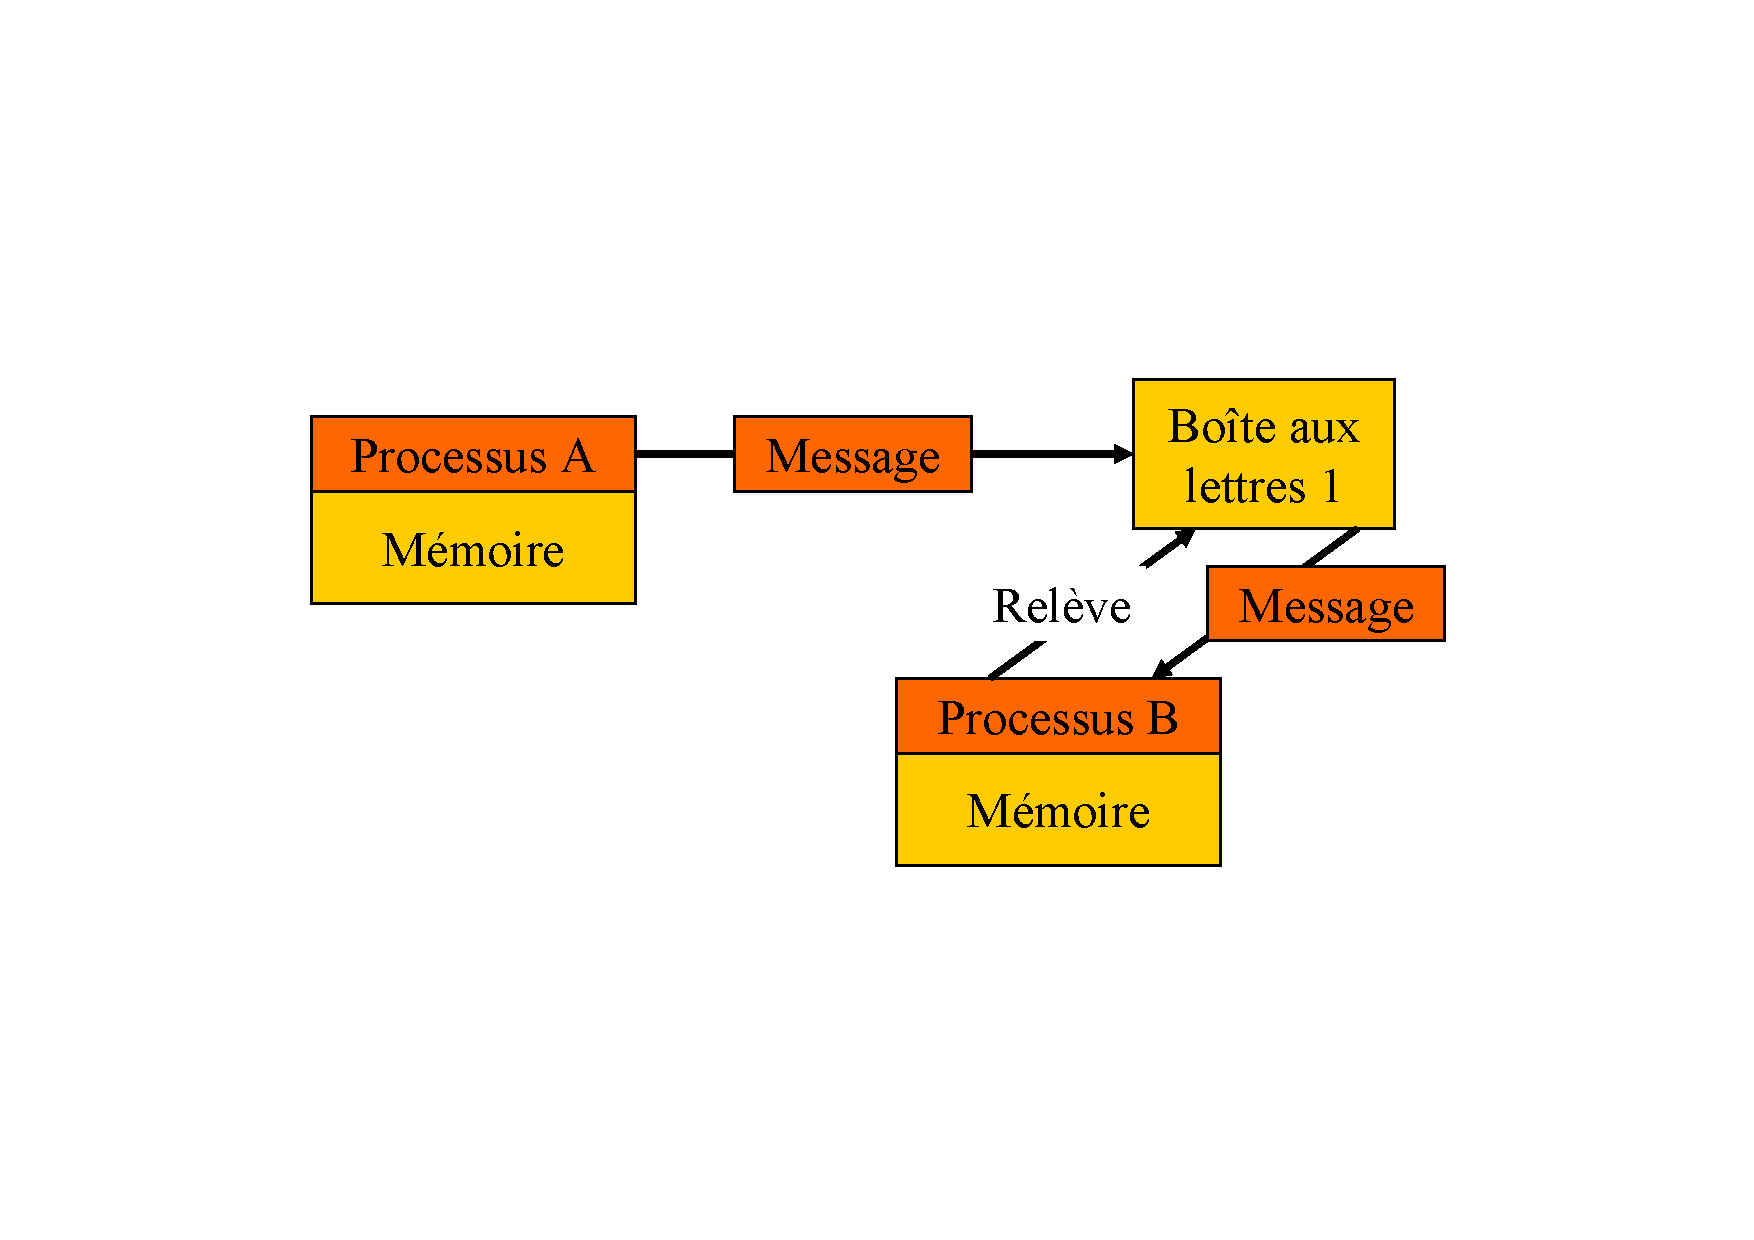
\includegraphics[width=.9\textwidth]{../illustration/comm_indirecte.pdf}
\begin{itemize}
\item A envoi un message à la BAL 1
\item B relève les messages de la BAL 1 (en la vidant)
\end{itemize}
\end{frame}

\begin{frame}
\frametitle{Communication indirecte}
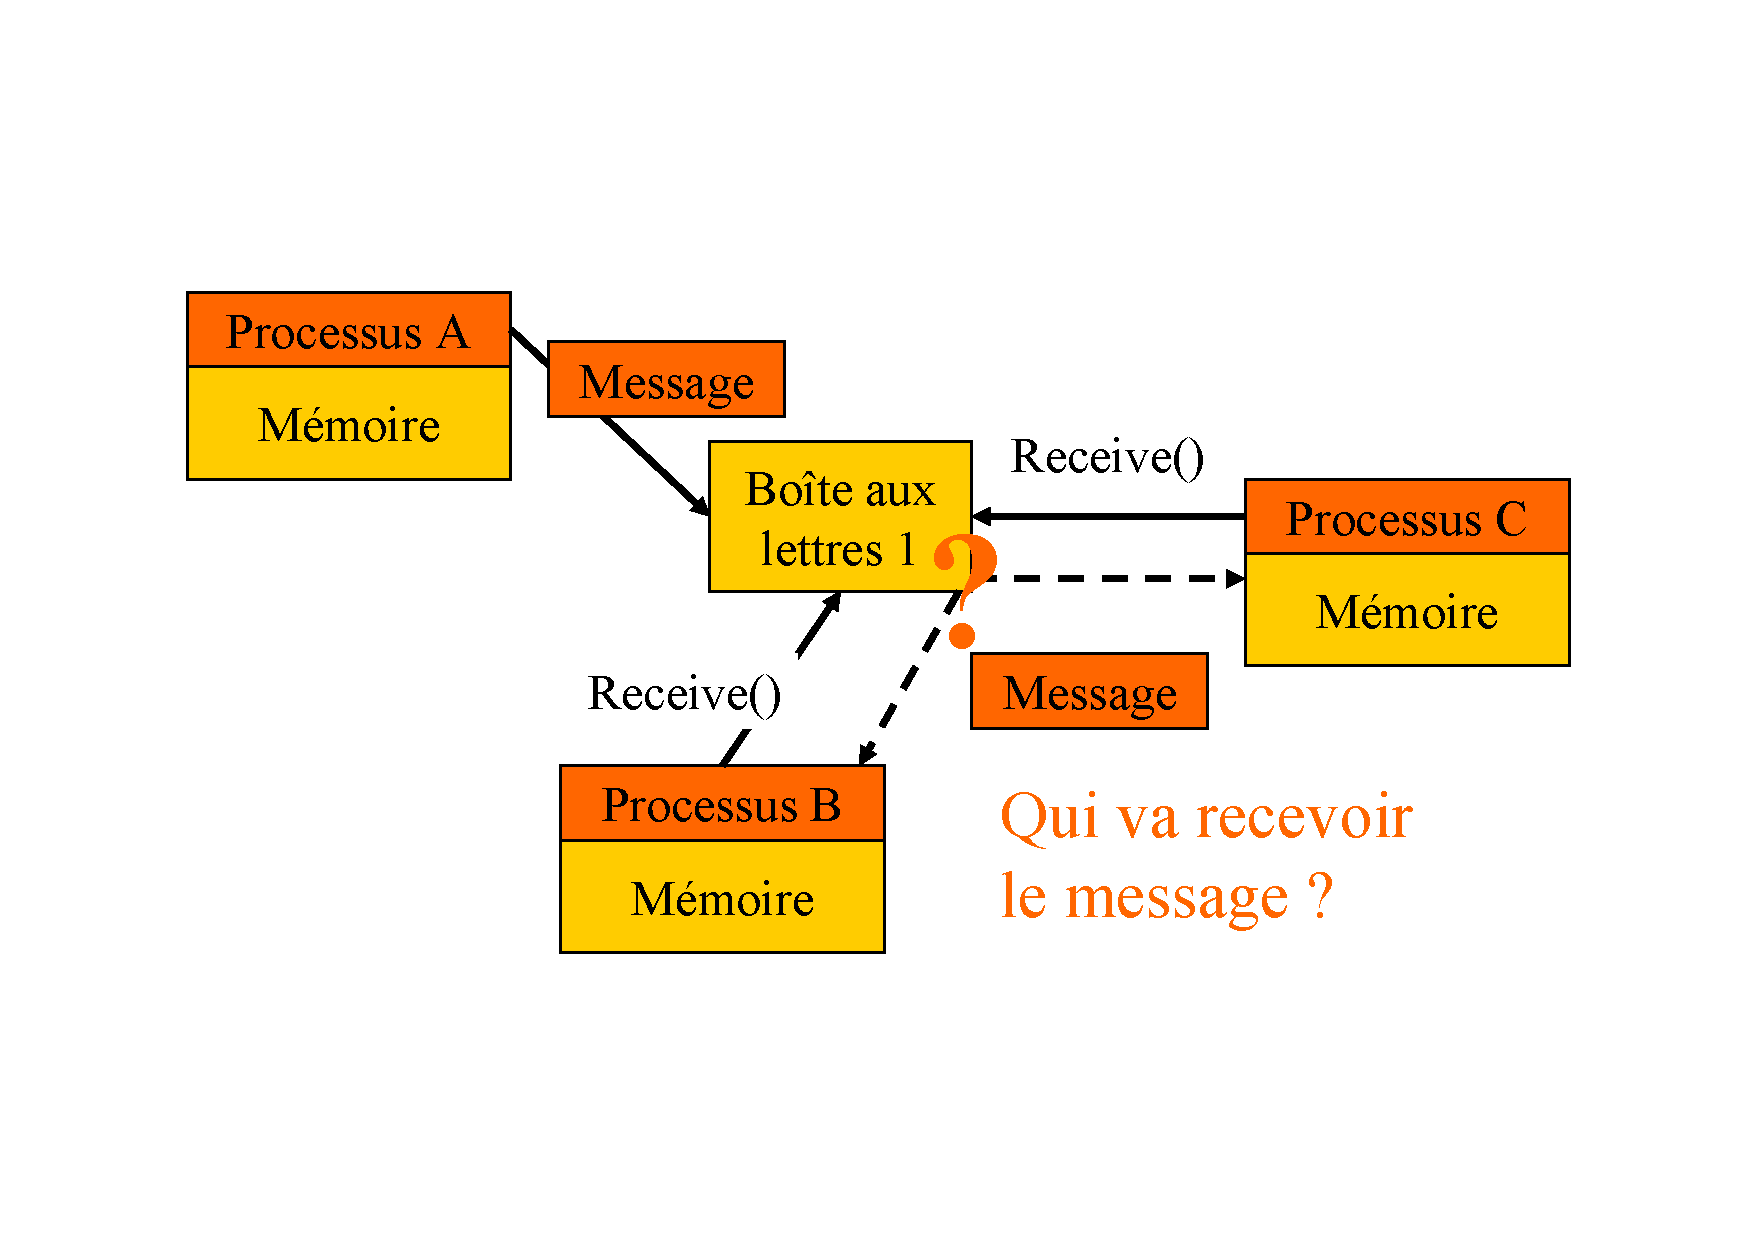
\includegraphics[width=.9\textwidth]{../illustration/comm_indirecte_question.pdf}
\end{frame}

\begin{frame}
\frametitle{Communication indirecte}
\begin{itemize}
\item Un boîte aux lettres peut appartenir à un processus ou au système
\item BAL d’un processus :
\begin{itemize}
\item Le processus est propriétaire de la BAL
\item Il ne peut que lire les messages de la BAL
\item Les autres processus ne peuvent qu’envoyer des messages dans la BAL
\item Disparaît avec le processus
\end{itemize}
\end{itemize}
\end{frame}

\begin{frame}
\frametitle{Communication indirecte}
\begin{itemize}
\item BAL du système :
\begin{itemize}
\item Indépendante de tout processus
\item Le système fourni les mécanismes pour :
\begin{itemize}
\item Créer une BAL
\item Envoyer et recevoir des messages d’une BAL
\item Supprimer une BAL
\end{itemize}
\item Processus qui crée la BAL en est le propriétaire par défaut
\begin{itemize}
\item Possibilité d’ouvrir les droits d’accès
\end{itemize}
\end{itemize}
\end{itemize}
\end{frame}

\begin{frame}
\frametitle{Communication indirecte}
\begin{itemize}
\item Synchronisation des communications
\begin{itemize}
\item Envoi bloquant
\item Envoi non bloquant
\item Réception bloquante
\item Réception non bloquante
\end{itemize}
\item Si envoi et réception bloquants :
\begin{itemize}
\item Rendez-vous entre émetteur et récepteur
\end{itemize}
\end{itemize}
\end{frame}

\begin{frame}
\frametitle{Communication indirecte}
\begin{itemize}
\item Message envoyés placés dans une file d’attente :
\begin{itemize}
\item Capacité nulle :
\begin{itemize}
\item Aucun message en attente
\item Émission bloquante
\end{itemize}
\item Capacité bornée :
\begin{itemize}
\item Processus émetteur bloqué si le tampon est plein
\end{itemize}
\item Capacité non bornée :
\begin{itemize}
\item L’émetteur n’est jamais bloqué.
\end{itemize}
\end{itemize}
\end{itemize}
\end{frame}

\begin{frame}
\frametitle{Exemple : micro noyau Mach}
\begin{itemize}
\item Noyau de système d'exploitation
\begin{itemize}
\item Libre et gratuit
\item Ecrit en C
\item Orienté objet
\end{itemize}
\item Une des premières implémentations réussies des micro-noyaux
\begin{itemize}
\item Portable
\item Temps réel
\item Niveau B3 des critères de sécurité du standard TCSEC\footnote{Trusted Computer System Evaluation Criteria}
\end{itemize}
\item Utilisé par de nombreux systèmes
\begin{itemize}
\item Hurd (micro-noyau) de GNU - remplacé par L4 depuis 2004
\item MkLinux, développé par Apple en 1996
\item XNU, noyau de Darwin, base de Mac OS X ($\ne$ micro-noyau)
\end{itemize}

\end{itemize}
\end{frame}

\begin{frame}
\frametitle{Exemple : Mach}
\begin{itemize}
\item Système d’exploitation à micro noyau basé sur les messages
\item Gestion de processus multi-threads
\item Micro-noyau
\begin{itemize}
\item Dialogue entre processus utilisateur et serveurs
\item Pas de partage d’espace d’adressage
\item Conçu pour les environnements distribués
\end{itemize}
\end{itemize}
\end{frame}

\begin{frame}
\frametitle{Exemple : Mach}
\begin{itemize}
\item Communications par messages :
\begin{itemize}
\item Appels systèmes
\item Boîtes aux lettres (ports)
\end{itemize}
\item Pour chaque processus, deux BAL spéciales :
\begin{itemize}
\item \textbf{Kernel} : Utilisée par le noyau pour communiquer avec le processus utilisateur
\item \textbf{Notify} : Notification d’avènement au processus utilisateur par le noyau
\end{itemize}
\end{itemize}
\end{frame}

\begin{frame}
\frametitle{Exemple : Mach}
\begin{itemize}
\item Transfert de messages :
\begin{itemize}
\item \texttt{msg\_send} / \texttt{msg\_receive}
\item \texttt{msg\_rpc} : Appel de procédure distante
\end{itemize}
\item Création de port :
\begin{itemize}
\item \texttt{port\_allocate}
\end{itemize}
\item Performances (transfert de message)
\begin{itemize}
\item Pas de duplication des messages en mémoire
\item Transfert de l’espace d’adressage contenant le message d’un processus à l’autre
\end{itemize}
\end{itemize}
\end{frame}

\begin{frame}
\frametitle{Exemple : Windows NT}
\includegraphics[width=.9\textwidth]{../illustration/exemple_winnt.pdf}
\end{frame}

\begin{frame}
\frametitle{Exemple de signaux asynchrones}
\framesubtitle{Windows NT}
\begin{itemize}
\item <1->Fonctionnalité d’appel de procédure locale (LPC)
\item <2->Communication avec les sous-systèmes
\begin{itemize}
\item Utilisation d’un canal de communication
\item Basé sur des ports (BAL)
\end{itemize}
\item <3->Deux types de ports :
\begin{itemize}
\item [Connexion] visible de tous, permet d’initialiser une communication
\item [Communication] permet le transfert d’informations
\end{itemize}
\end{itemize}
\end{frame}

\begin{frame}
\frametitle{Exemple de signaux asynchrones}
\framesubtitle{Windows NT}
\begin{block}{Déroulement d'une communication}
\begin{itemize}
\item <1->Identification port de connexion du serveur
\item <2->Émission requête vers ce port
\item <3->Création de deux ports de communication privés par le serveur :
\begin{itemize}
\item Du serveur vers le client
\item Du client vers le serveur
\end{itemize}
\item <4->Communication client-serveur via ces ports
\end{itemize}
\end{block}
\end{frame}

\frame[allowframebreaks]
{
\frametitle{Bibliographie}
\bibliographystyle{plain}
\bibliography{smb137}
}

\end{document}
